%%% File encoding: UTF-8
%%% äöüÄÖÜß  <-- no German umlauts here? Use an UTF-8 compatible editor!

%%% Magic comments for setting the correct parameters in compatible IDEs
% !TeX encoding = utf8
% !TeX program = pdflatex 
% !TeX spellcheck = en_US
% !BIB program = biber

\documentclass[master,english,smartquotes]{hgbthesis}
% Valid options in [..]: 
%    Type of work: 'diploma', 'master' (default), 'bachelor', 'internship' 
%    Additionally for a thesis exposé: 'proposal (for 'bachelor' and 'master')
%    Main language: 'german' (default), 'english'
%    Turn on smart quote handling: 'smartquotes'
%    APA bibliography style: 'apa'
%%%-----------------------------------------------------------------------------

\RequirePackage[utf8]{inputenc} % Remove when using lualatex or xelatex!

\graphicspath{{images/}}  % Location of images and graphics
\logofile{logo}           % Logo file: images/logo.pdf (no logo: \logofile{})
%\bibliography{references} % BibLaTeX bibliography file (references.bib)
\bibliography{bibliography} % BibLaTeX bibliography file (references.bib)

%%%------------------------------ custom packages ------------------------------
\usepackage[colorinlistoftodos]{todonotes}
\usepackage{epigraph}
\usepackage{svg}
\usepackage{threeparttablex} % for "ThreePartTable" environment
\usepackage{booktabs}        % for well-spaced horizontal rules
%%%-----------------------------------------------------------------------------

\newcommand{\addref}{\todo[color=red!40]{Add reference.}}
\newcommand{\estimatedpagecount}[1]{\todo[color=blue!40]{Estimated Pages: #1}}
\newcommand{\CS}{C\nolinebreak\hspace{-.05em}\raisebox{.6ex}{\scriptsize\bf \#}}
\newcommand{\textgreek}[1]{\begingroup\fontencoding{LGR}\selectfont#1\endgroup}

%%%-----------------------------------------------------------------------------
\begin{document}
%%%-----------------------------------------------------------------------------

%%%-----------------------------------------------------------------------------
% Title page entries
%%%-----------------------------------------------------------------------------

%\title{Partial Solutions to Universal Problems}
\title{%
  Towards Hole-Driven Development in General Purpose Programming Languages \\
  \large A Proof of Concept in C\#}
\author{Bernhard Mayr}
\programname{Mobile Computing}

%\programtype{Fachhochschul-Bachelorstudiengang} % select/edit
\programtype{Fachhochschul-Masterstudiengang}

\placeofstudy{Hagenberg}
\dateofsubmission{2023}{06}{27} % {YYYY}{MM}{DD}

\advisor{FH-Prof. DI Stephan Selinger} % optional

%\strictlicense % restrictive license instead of Creative Commons (discouraged!)

%%%-----------------------------------------------------------------------------
\frontmatter                                   % Front part (roman page numbers)
%%%-----------------------------------------------------------------------------

\maketitle
\tableofcontents

\listoftodos

%\chapter{Preface}
Finishing this thesis took longer than anticipated.
There is a bit of backstory to this.
After completing my first bachelor's in software engineering, I started another bachelor's in psychology, which sparked my interest in combining those seemingly contradictory research areas.
I started researching the topic of holes in programming when I wrote my bachelor's thesis in psychology about the possibilities of combining holes with Statecharts.

Shortly after this, I joined the fantastic people at StateML, where we are researching a language for modeling event-driven behavior in our spare time.
Thank you, Chris, John, and Owen, for the countless hours of discussions about the history of software, non-conventional ideas of approaching software, and what we can learn from this.
We already integrated some ideas around holes into StateML; therefore, I initially started working on this thesis to show how to apply Hole-Driven Development to Statecharts.
However, your immense focus on composability reshaped my view of holes.
As such, this thesis is about creating a framework for composable holes instead of applying it to Statecharts directly.
But this idea is not forgotten; it was simply turned into a hole to be filled later on.

Parts of the core idea of this thesis have already been presented at Mensch und Computer (MuC) 23 and published in \cite{mayr_replacing_2023}.
Thank you, Marc, for motivating me to submit at MuC, providing feedback about my ideas, and for a great time in Switzerland.

Prior to presenting at MuC, I attended the Psychology of Programming Interest Group's (PPIG) 34th annual workshop in Lund, Sweden.
Thank you, Clayton, Luke, Leah, Anton, and Görel, for your input, and Alan, for your exceptional defense and the conversational perspective regarding programming.

Speaking of input, many ideas are born, enhanced, rejected, and validated at this inspiring monthly round table with Alex, Dominik, Georg, Sebastian, and Stefan.
You played a big part in why I returned to software development and still stick around; thanks for all the inspiring conversations about everything.

The people who have probably been most affected by my writing this thesis are my family, flatmates, and friends.
Thank you for all your support and sorry for the times I've been unresponsive, especially Mom, Tinka, Mona, Jakob, Rosa, Daniel, David, and Marlene!

I feel really privileged that my dad had the greatest influence on this thesis.
He challenges my beliefs, lets me challenge his, and can give me hints about decades of experience in software engineering.
He is also the best proofreader, knowing so many details about grammar, scientific writing, and the topics of not only my technical writings - thank you, Dad!

This thesis would not have been possible without my supervisor Stephan Selinger.
Thank you for your input, patience, trust, and flexibility, and for supervising a thesis unrelated to machine learning or large language models in 2023.
I could still not imagine doing an Ironman after completing the 100km trail run, but I've got the feeling that writing this thesis might have brought me a little bit closer.

\vspace{6ex}
\noindent
B.\ Mayr % A preface is optional
\chapter{Abstract}
Live programming allows users to interactively explore programs for a better understanding and more accurate mental model.
Furthermore, shorter feedback loops enable programmers to stay focused while being able to iterate on new ideas quickly.
Shortening feedback loops by incorporating feedback as early as possible also led to the agile movement for software engineering processes, which values collaborating individuals and interactions over processes and tools.
However, as live programming shows, tools can support various ways of interaction.
As such, they can aid the complex problem-solving task of programming by reducing the cognitive load that stems from translating complex requirements into working software.
Developing prototypes helps to create a shared understanding between developers and stakeholders by showing how the product under development behaves.
However, widely used general-purpose programming languages are not optimized for tight feedback loops and interactive prototypes that evolve into production-grade software.

Viewing the process of programming as one of conversing with stakeholders, oneself, and the compiler, we looked at existing solutions that target dealing with cognitive load as well as tightening feedback loops and applied these findings to widely used general-purpose programming languages.
Based on todo comments, applications of Hole-Driven Development, and creative ways of simulating holes, we identified 13 properties intrinsic to using holes in programming.
Based on these properties, we developed \emph{Holey}, a proof of concept for applying the ideas of Hole-Driven development to the widely used general-purpose programming language \CS.
This proof of concept can be used to investigate possible advantages regarding the usability and applicability of writing incomplete, but executable and evolvable software.

\chapter{Kurzfassung}

\begin{german} %switch to German language rules
	Dies sollte eine maximal 1-seitige Zusammenfassung Ihrer Arbeit in deutscher
	Sprache sein.
	%here goes the rest of the Kurzfassung...
\end{german}

The German "Kurzfassung" should contain the same content as the English abstract.
Therefore, try to translate the abstract precisely but not word for word. When
translating, remember that certain idioms from English have no counterpart in
German or must be formulated differently. Also, word order in German is very
different from English (more on this in Section \ref{sec:german}). Without
knowledge of the German language, it is acceptable to resort to translators.
Nevertheless, hiring a skillful person for proofreading is recommended
even with the highest confidence in one's German knowledge.

The correct translation for "diploma thesis" is \emph{Diplomarbeit}, a "master
thesis" is called \emph{Masterarbeit}. For "bachelor's thesis",
\emph{Bachelorarbeit} is the appropriate translation.

By the way, for this section, the \emph{language setting} in \latex\ should be
switched from English to German to get the correct form of hyphenation. However,
the correct quotation marks must be set manually (see Sections
\ref{sec:language-switching} and \ref{sec:quotation-marks}).


%%%-----------------------------------------------------------------------------
\mainmatter                                    % Main part (arabic page numbers)
%%%-----------------------------------------------------------------------------

\chapter[Introduction]{Introduction \protect{\estimatedpagecount{16}}}
\epigraph{How do we get people to understand programming?}{Bret Victor}

The idea of learnable programming \cite{victor_learnable_2012} goes back to the early days of Smalltalk \cite{kay_early_1993}.
In his essay \emph{The Early History of Smalltalk}, Alan Kay looks back at the events that led to the creation of Smalltalk.
More importantly, he gives insight about the context of why Smalltalk turned out how it did.
Smalltalk was intended to be a learning environment for children, side-effects like its strong object orientation were merely artifacts of this main idea \cite{kay_early_1993}.
Objects, message passing and compositionality allowed people (not only children) using Smalltalk, to align their ways of thinking with the way their programs were structured.
Applying the conversational lens of programming environments (see Section~\ref{sec:conversational-lens}) to Smalltalk, one could argue that speaking the same language results in a shared mental model between the program and the programmer.
Or as Weinberg \cite{weinberg_psychology_1971} described the status quo (in 1971): "When we talk to our computers, unhappily, we are usually speaking in different tongues."
Unfortunately, not a lot of effort has been put into aligning those tongues over the last 50 years.

Programming environments that foster this style of communication are usually called live programming\cite{aguiar_live_2019, church_liveness_2010} or interactive programming \cite{czaplicki_interactive_2013, mccabe_towards_2023}.
Usually, such systems possess the following properties \cite{burg_1st_2013}:
\begin{description}
    \item[Live] They give the programmer immediate feedback, while the program is edited. This feedback can target its output, structure or both.
    \item[Structured] Environments which are aware of a program's structure, understand and preserve this structure. They operate at the level of structure, not on raw text.
    \item[Tangible] Normally, program execution happens behind the scenes and provides little to no capabilities for live inspection. Tangible programming makes the execution transparent, tangible and explorable.
    \item[Concrete] It is way easier for people to start with concrete examples and generalize later on.
\end{description}

Live programming systems lead to tighter feedback loops.
This outcome was described by Chris Hancock \cite{hancock_real-time_2003} and illustrated in \cite{aguiar_live_2019} as shown in Figure~\ref{fig:bow-arrow} and Figure~\ref{fig:waterhose}.
%
\begin{figure}[h]
\centering
\includesvg[width=0.75\textwidth]{images/arrow-bow}
\caption{When trying to hit a target with bow and arrow one can only re-aim based on the previous shot. Feedback is provided only after the arrow reaches the target. Image source~\cite{aguiar_live_2019}.}
\label{fig:bow-arrow}
\end{figure}
%
There are multiple differences in trying to hit a target with bow and arrow vs. with a hose.
The most obvious one is the constant stream of information that is provided by observing where the water hits the target in the second analogy.
But is this uninterrupted stream of information really the reason why it is easier to hit a target with a hose?
Hancock \cite{hancock_real-time_2003} argues that this is only a fraction of the reason, according to his interpretation the main difference is that the waterer \emph{never stops aiming}.
While the archer's actions consist of a series of distinct actions (while having to re-aim after each shot), the waterer does not have to "reload".
Hence the waterer does not need to switch contexts, while at the same time being supported by continuous feedback.
One can also visually perceive the shortened feedback loop between Figure~\ref{fig:bow-arrow} and Figure~\ref{fig:waterhose}.

\begin{figure}[h]
\centering
\includesvg[width=0.6\textwidth]{images/waterhose}
\caption{Aiming with a hose is much easier. Continuous feedback allows the person using the hose to constantly re-adapt to the target, without having to stop aiming at all. Image source~\cite{aguiar_live_2019}.}
\label{fig:waterhose}
\end{figure}

In contrast to the previously described problem of speaking the same tongue, several frameworks and programming tools are actively trying to shorten the feedback loop \cite{kubelka_road_2018}.
Web development tools in major browsers support direct page editing \addref, Vitest, a testing framework for JavaScript supports an instant watch mode \addref, all major web frameworks support hot-module reloading \addref, qwik lets developers click at components which takes them directly to the source code \addref. Redux allows developers to travel through their application state by providing time-travelling debugging \addref.
REPLs are kind of standard for newly developed languages \addref, Java and .NET support hot-reloading under certain circumstances \addref and Apple's Swift programming language supports live programming with interactive playgrounds \addref.
Although this list is by far not exhaustive and there is a clearly visible trend towards live programming, comparing tools used in industry to the properties of live programming, there is still a huge gap.
The next section portraits the concept of interactive programming in the broader context of software development, compared to "just" programming.



\todo[inline,color=blue!40]{Maybe cross-reference to Psychology of Programming and explain that faster feedback fosters happiness.}
\todo[inline]{Explain that industry is slowly adopting these ideas (based on [Kubelka.etal:2018]).}
\todo[inline]{Argue that there is much better we can do, and this is the content of this thesis. Then transition to the context of the thesis.}


15 checklists
111 memory


\section[Context]{Context \protect{\estimatedpagecount{3.5}}}
\todo[inline]{This feedback-loop metaphor can be applied to a specific developer, a team or even with customer-interaction.}
\todo[inline]{In the introduction I did not differentiate between programming and software development, but it is a huge differentiation.}
\todo[inline]{Explain the differences between psychology of programming and psychology of software development and what it has to do with requirements to code and idea to code.}

\subsection[Agile Movement]{Agile Movement \protect{\estimatedpagecount{1.5}}}
\todo[inline]{Give an overview on the development of agile ideas and how it has changed the tasks of software developers.}
\todo[inline]{Use the arrow/firehose analogy to mentally visualize the faster iteration cycles leading to tighter feedback loops}
\todo[inline]{Software has to be developed faster, the requirements are defined more dynamically - mention theory vs. reality}
\todo[inline]{Bring the concept of tactical programming vs. strategic programming into play (based on Osterhout as described in my Psychology BA)}
\todo[inline]{Transition to the next chapter by highlighting the importance of prototypes in agile development.}
\todo[inline,color=blue!40]{Maybe look into Rapid Application Development and its approach on Prototyping}

\subsection[Prototyping]{Prototyping \protect{\estimatedpagecount{1.5}}}
\todo[inline]{Start with the etymology of the word prototype, based on greek proto + typos.}
\todo[inline]{Explain how prototyping works in reality and what evolutionary prototyping is. (with the figure from my AmA talk)}
\todo[inline]{Mention that prototypes get released to production (Tesla, Spotify, Apple) and that customers do the testing.}
\todo[inline]{Show this contradiction with the etymological approach.}
\todo[inline,color=blue!40]{Maybe bring in a little bit of capitalism criticism in the form of market fit vs. high-quality products, just show the contradiction.}
\todo[inline]{Transition to wizard of oz prototyping and how this is actually prototyping, but show its complexity and the difference between the prototype and the actual product.}

\subsection[Interactive Programming]{Interactive Programming \protect{\estimatedpagecount{.5}}}
\todo[inline]{Bridge the gap between prototyping and interactive/live programming as described in the introduction. Mention how this might align with agile methodologies, the psychology of programming and customer-centered approaches.}



\section[Problem Statement]{Problem Statement \protect{\estimatedpagecount{6}}}
\todo[inline]{Based on the context, explain the contradictions once more and re-phrase them as the problem statement of this thesis.}

\subsection[Programming as Complex Problem Solving]{Programming as Complex Problem Solving \protect{\estimatedpagecount{4}}}
\todo[inline]{Use material from the Psychology BA to show similarities between research on complex problem solving and programming.}

\subsubsection[Top-Down vs. Bottom Up]{Top-Down vs. Bottom Up \protect{\estimatedpagecount{1.5}}}
\todo[inline]{Explain top down and bottom up processes and how they problem solving applies to it via functional (de-)composition.}
\todo[inline]{Create figures that look like fractal pyramides, one approaching from top, one approaching from bottom.}
\todo[inline]{"To use the bottom up method you need to be able to efficiently determine what the "bottom" is, which usually means you need a heavily constrained problem space."}
\todo[inline,color=green!40]{relevant literature: \cite{kung_comparing_2013}}
% \url{https://en.wikipedia.org/wiki/Bottom%E2%80%93up_and_top%E2%80%93down_design}
% \url{https://www.geeksforgeeks.org/difference-between-bottom-up-model-and-top-down-model/}

\subsubsection[Programming as Theory Building]{Programming as Theory Building \protect{\estimatedpagecount{1.5}}}
\label{sec:programming-as-theory-building}
\todo[inline]{Deep dive into Peter Naur's perspective on programming and why theory building explains why software is hard to maintain.}
\todo[inline]{Maybe bring the example of the Compiler for showing how communication is such an important aspect of software development.}
\todo[inline]{\textbf{Basically sum up his paper in one and a half pages, cause it is so fundamental to this research.}}
\todo[inline,color=green!40]{relevant literature: \cite{naur_programming_1985}}

% In a very simplistic view, programming can be seen as the act of converting requirements to source code.
% With this task being carried out by people, one could look at psychology's research field of complex problem-solving and apply it to programming.
% There is not a lot of active research being conducted in this area, but Weinberg \cite{Weinberg:1971} and Naur \cite{Naur:1985} did some fundamental research combining psychology's complex problem solving and the act of programming.
% In his essay \emph{Programming as Theory Building} \citet{Naur:1985} hypothesized that programs are more than just their textual artifacts.
% Instead, individuals, as well as teams create a shared understanding of the problem they have to solve.
% Programming is about creating this understanding, hence improving programming is about improving the creation of this understanding, thus improving communication.

% Communication does not only happen in teams.
% Someone, developing something that can not be accomplished in a few minutes, needs to communicate with oneself as well as the computer.
% Decomposing requirements, keeping track of them, discovering bugs, and transforming code changes are just some of the tasks that might need some form of communication.
% Quite a lot of this communication happens via code comments \cite{Ying.etal:2005}.
% Comments are not only used for documentation purposes, but as well to make notes of things that have to be changed or considered.
% In contrast to the parts of source code that are actually run, comments are informal and not bound to any syntax rules, making them hard to parse and interpret for machines.
% This leads to comments being forgotten quite frequently \cite{Nie.etal:2019}.
% Preventing their forgetting and actually making use of them for the act of programming is the main motivation for this research.

\subsubsection[Conversational Lens regarding Complex Problem Solving in Development]{Conversational Lens regarding Complex Problem Solving in Development \protect{\estimatedpagecount{1}}}
\label{sec:conversational-lens}
\todo[inline,color=purple!40]{"Programs are used not only for man-machine communication, but for man-man communication as well."}
\todo[inline]{Sum up Alan's ideas regarding looking at programming through the conversational lens and how the idea of communication can be applied to IDEs.}
\todo[inline]{Also put this conversational lens idea into perspective regarding conversations between people, like already done in the MuC paper and described in \ref{sec:programming-as-theory-building}.}
\todo[inline,color=green!40]{relevant literature: \cite{mccabe_towards_2023}}

\subsection[Mental Load]{Mental Load \protect{\estimatedpagecount{2.5}}}
\todo[inline]{Check what "Code that fits in your Head" can attribute to this section}
\todo[inline]{Dive a bit into the psychology of programming and its research on \emph{working memory capacity}}
\todo[inline]{Present the research about Post-Its}
\todo[inline,color=blue!40]{Maybe look into the psychological implications like stress, anxiety and other disorders}
\todo[inline,color=green!40]{relevant literature: \cite{digiano_learning_nodate, seemann_code_2021}}



\section[Hypothesis]{Hypothesis \protect{\estimatedpagecount{4}}}
\todo[inline]{Transition to the hypothesis section of this paper, because of it being a Proof of Concept}

\subsection[About Todo-Comments]{About Todo-Comments \protect{\estimatedpagecount{2.5}}}
\todo[inline]{Start with an introduction on scientific results regarding Todo comments}
\todo[inline]{Do a short qualitative analysis regarding the various stackexchange posts on Todo-Comments}
\todo[inline,color=blue!40]{If I manage to find, I intend to include some statistics on Todo-Comments}
% - \url{https://www.petermorlion.com/the-lifetime-of-todo-comments-the-results/}
% - Tickgit
\todo[inline,color=blue!40]{Maybe try to group and order these into separate categories/quantitites, or report them by stackexchange question/discussion}
% - https://softwareengineering.stackexchange.com/questions/175719/can-notes-to-dos-in-code-comments-sent-to-code-reviews-result-in-an-effective-re
% - \url{https://softwareengineering.stackexchange.com/questions/323498/why-is-having-a-notimplementedexception-a-good-thing#comment687389_323498}
% - https://softwareengineering.stackexchange.com/questions/125320/do-todo-comments-make-sense
% - https://stackoverflow.com/questions/1989177/how-to-manage-todo-programming-stuff
% - https://stackoverflow.com/questions/16913055/how-can-i-mark-to-do-comments-in-xcode
% - https://stackoverflow.com/questions/335378/how-do-you-flag-code-so-that-you-can-come-back-later-and-work-on-it
\todo[inline,color=green!40]{relevant literature: \cite{nie_natural_2018, ying_source_2005, nie_framework_2019, sridhara_automatically_2016, storey_todo_2008, storey_how_2009}}

\subsection[Introducing Hole-Driven Development]{Introducing Hole-Driven Development \protect{\estimatedpagecount{1.5}}}
\todo[inline]{Start with the \emph{Fill in the Blank Exercise} analogy, then continue with an example}
\todo[inline]{Quickly show the Idris example, but mainly reference the related work section}

\section[Research Question and Methodology]{Research Question and Methodology \protect{\estimatedpagecount{1.5}}}
\todo[inline]{Lay out the process of approaching this thesis}
\todo[inline]{It mainly consists of deducing the requirements based on literature (reference the according chapter in related work), and validating the results according to the already supported concepts of Hole-Driven Development}
\todo[inline]{\emph{This work represents a proof of concept for applying the concept of hole-driven development to general-purpose programming languages, in this case \CS.}}
\todo[inline]{\emph{Which aspects of existing Hole Implementations can be transferred to general-purpose (mainstream) programming languages? With the requirements being laid in Sec 2.4 out after analyzing those in Sec 2.}}

\section[Structure of the Thesis]{Structure of the Thesis \protect{\estimatedpagecount{.5}}}
\todo[inline]{Quickly describe the structure of the thesis.}
\chapter[Related Work]{Related Work \protect{\estimatedpagecount{15}}}
\epigraph{We should think of the compiler as being our lab assistant.}{Edwin Brady}

\section[Tackling Todo-Comments]{Tackling Todo-Comments \protect{\estimatedpagecount{4}}}
\todo[inline,color=blue!40]{Mention again that Todo-Comments tend to rot}
\todo[inline]{Shortly explain the usage of Todo-Comments again, before mentioning that there are a couple of other tools as well that tackle the problem of Todo comments}
\todo[inline]{Hightlight PEP--350 Codetags and TrigIt, because of their novel approaches regarding Todo-Comments}

\subsubsection{PEP--350 Codetags}
% - \url{https://medium.com/hackernoon/never-forget-anything-before-after-and-while-coding-98d187ae4cf1#.czqio0b4x}
\subsubsection{TrigIt}
\subsubsection{TagSEA \cite{storey_how_2009}}
\subsubsection{Tickgit}
\subsubsection{Catana}
\subsubsection{imdone}
\subsubsection{Editor Integrations}
\subsubsection{Editor Plugins}



\section[Languages with native Holes support]{Languages with native Holes support \protect{\estimatedpagecount{6}}}
\todo[inline]{Mention that a couple of languages natively support the concept of Holes}
\todo[inline]{\textbf{make sure that those are sorted by invention date}}

\subsubsection{Coq}

\subsubsection{Agda}

\subsubsection{Haskell}
\todo[inline,color=blue!40]{maybe do some research regarding Liquid Haskell}

\subsubsection{Hazel}
%https://www.youtube.com/watch?v=UkDSL0U9ndQ
%the gap problem
%what you start with is a hole
%what should we fill this hole with (in-class)
%regarding machine learning: having a theory of incomplete programs allows us to do it this way
%splicing: putting holes inside text

\subsubsection{Idris}

\section[Simulating Holes in other Languages]{Simulating Holes in other Languages \protect{\estimatedpagecount{5}}}
\subsubsection{\CS}
\todo[inline]{NotImplementedException}
\todo[inline]{dynamic}
\todo[inline,color=green!40]{relevant literature: \cite{microsoft_notimplementedexception_2020}}

\subsubsection{Java}
\todo[inline,color=green!40]{relevant literature: \cite{omar_active_2012}}

\subsubsection{Scala}
\todo[inline]{???}
\todo[inline,color=green!40]{relevant literature: \cite{odersky_adding_2011}}

\subsubsection{Swift}
\todo[inline]{do some research on this}

\subsubsection{Rust}
\todo[inline]{!todo}
\todo[inline]{!unimplemented}

\subsubsection{TypeScript}
\todo[inline]{Mention that the difference here is that we apply Holes at the type level}
\todo[inline]{Explain the idea of gradial refinement}
\todo[inline]{any + NoImplicitAny}
\todo[inline]{unknown}
\todo[inline]{eslint}

\subsubsection{\LaTeX}
\todo[inline]{explain how todo comments can be used while writing a \LaTeX document}
\todo[inline]{Mention the properties of a couple of \LaTeX-packages: todonotes, easy-todo, fixmetodonotes, todo, fixme}
\todo[inline]{Highlight the comments on ctan (for the todonotes-package) of how useful todos are when collaborating on a document}
%- https://ctan.org/pkg/todonotes
%- https://ctan.org/pkg/easy-todo
%- https://ctan.org/pkg/fixmetodonotes
%- https://ctan.org/pkg/todo
%- https://ctan.org/pkg/fixme
%  - \#Controlling the behavior of FiXme shows the idea of Release/Debug mode

\section{Properties of Holes}
\todo[inline]{Refer to Cyrus Omar's talk about Hazel regarding the properties of Holes as a basis}
\todo[inline]{Then cautiously add the other properties of Holes discovered in the literature research}
\begin{description}
   \item[Holes DSL] A \CS-internal domain specific language to construct holes, which is loosely based on PEP 350 -- Codetags \cite{elliott_pep_2005}, \textsc{TrigIt} \cite{nie_framework_2019} and the comment types identified in \cite{ying_source_2005}.
   \item[Executability] The main promise of hole-driven comments is their executability. One should be able to already run an under-specified program and choose some of the unspecified behavior at runtime.
   \item[Hole Reporting] To provide value to the programmer, the holes need to be reported. Roslyn Analyzers provide capabilities to analyze the source code and report errors independent of the used editor. These can be used to detect and report the holes.
   \item[Build Differentiation] Enabling simulation capabilities can be implemented by supporting different configurations in different build variants. As an example, users might want to simulate holes in a debug build while breaking the release build due to under-specified behavior.
   \item[Support Mocking Libraries] Providing data at run-time might not always be the best solution (e.g. timing issues, no user interface, $\dotsc$), so users should be able to integrate external mocking libraries that provide the data.
   \item[Refactoring Integrations] Based on Roslyn's analyzers and code fixes, certain refactoring operations could be offered to developers. This should work like \textsc{TrigIt}'s code manipulations \cite{nie_framework_2019} or Idris' heuristics \cite{brady_type-driven_2017}.
   \item[Comment Transformation] Again, Roslyn should make it possible to analyze an existing project and transform existing TODO-comments into holes.
\end{description}
\chapter[Implementation]{Implementation \protect{\estimatedpagecount{20}}}
\label{cha:implementation}
\epigraph{What runs, the code or the comments?}{Brian Kernighan}

\todo[inline]{Mention the idea of using idiomatic \CS, so that legacy projects can be supported}
\todo[inline]{Show the pathway on how this developed...}

\section{Types of Holes}
\subsection{Todo-Comment}
\todo[inline]{Explain the necessity of Todo-Comments, how they can look like and why it makes sense to support them in their purest way}

\subsection{Hole-Comment}
\todo[inline]{Explain the difference between Hole-Comments and Todo-Comments and what lifts a Todo-Comment in the Hole-Comment state}
https://goldin.io/blog/stop-using-todo

\subsection{Missing Implementation}
\todo[inline]{Reference the opening quote of this chapter}
% - https://softwareengineering.stackexchange.com/a/323503
\todo[inline]{Explain the concept of stub-generation by the IDE, why it makes sense, but why it is scary that those NotImplementedExceptions are only discovered at runtime}
\todo[inline,color=blue!40]{Maybe do a small excursion into the land of checked exceptions and the difference between \CS and Java}

\subsection{Side-Effect}
\todo[inline]{Show the missing piece of runtime holes and which power they provide.}
\todo[inline,color=blue!40]{Maybe already dive into the idea of abstract I/O and that getters and setters are enough to model side-effects}


\section[Architecture]{Architecture \protect{\estimatedpagecount{2}}}
\todo[inline]{Explain the overall architecture of the combination of a library, the analyzers and the VS Plugin}
\todo[inline]{Explain the difficulties in building a DSL in \CS, no functions, only static methods on classes}

\subsection{Architecture Overview}
\todo[inline,color=blue!40]{Maybe include a C4 diagram of the packages}

\subsection{Bridging static Contexts and DI}
\todo[inline]{Explain the difficulties of bridging the static context and DI}

\subsection{Supporting Logging}
\todo[inline]{Dive into .NET's mess of ILogger, ILogger<T> and ILoggerFactory and their usage in libraries}
\todo[inline]{Explain how this could be solved using StashBox}

\subsection{Language Independence}
\todo[inline]{Explain the modularity and how the \CS-solution might be transferred to other languages (e.g. Python, Java, TS)}
\todo[inline]{mention what is needed for other languages to adopt holes}

\section{Providing IDE Support}
\todo[inline]{Give a quick introduction into Roslyn Analyzers}
\todo[inline]{Explain how Roslyn Analyzers offer IDE-independent support}

\subsection[Analyzers]{Analyzers \protect{\estimatedpagecount{3}}}
\todo[inline]{Explain the implemented Analyzers}
\todo[inline]{Explain why it makes sense that debug and release mode are handled separately and how this was accomplished}
\todo[inline]{Connect this to TreatWarningsAsErrors}
\todo[inline]{Explain the difference to simple linters}

\subsection{Code Fixes}
\todo[inline]{Show the power and usability improvements that Code Fixes in combination with Analyzers provide}

\section{Bridging Compile- and Runtime}
\todo[inline]{Explain why it is necessary to bridge between compile- and runtime}

\subsection{Stacktraces}
\todo[inline]{Dig into the concept of Stacktraces and why they might be (but in reality can't) be used to get information about the running code}

\subsection{Compiler Generated Attributes}
\todo[inline]{Explain the usage of .NET's compiler generated attributes}
\todo[inline]{Also mention the downside of having to specify generics when strings are used}

\subsection{Source Generators}
\todo[inline]{Briefly explain \CS's version of source generators vs. T4 templates}
\todo[inline]{Explain how compile-time information can be lifted into runtime}

\section{Extensibility}
\todo[inline]{Focus on the importance of Extensibility for such an abstract concept/library}

\subsection{Reporting}
\todo[inline]{Explain how custom reporters can be utilized}

\subsection{Mocking}
\todo[inline]{Explain the pathway to prototype-mocking as well as why custom packages aren't necessary anymore}
\todo[inline]{Once again mention the concept of abstract I/O and how powerful this is}
\todo[inline]{Transition to the Sidecar Application}

\subsection{Sidecar Application}
\todo[inline]{Briefly explain that the Sidecar Application is no fundamental part of Holey, but it can be created solely on Holey's extensibility options}

\subsubsection{Communication}
\todo[inline]{Explain the abstracted communication channels and that they are not tied to anything else}

\subsubsection{Dynamic Form Generation}
\todo[inline]{Quickly dive into dynamic form generation and show all the code (because it is just one line per application)}
\todo[inline,color=blue!40]{Maybe also mention that the JSON Schema adapter can be switched to a custom one}

\chapter{Summary (7)}
\epigraph{Isn't that reverse hot-reloading?}{Stefan Baumgartner}
\section{Discussion}
\section{Contributions}
- new way of interacting with programs: reverse hot-reloading
- tightening the feedback loop
- applying HDD to general purpose PLs
\section{Applications}
- educational setting
- company setting (like described by Angie)
- dev2dev communication
- pontential customer involvement
\section{Limitations}
- vs. Test-Driven Development (\todo{Papa sein Input dazu finden und anwenden})
- vs. Linting
\section{Future Ideas}
- vueflow like Angie described
- CodeLLMs
- additional languages
- Sidecar with multiple applications
\section{Future Work}
\subsection{Ideas}
- LLMs
- Record and Replay
- Language
- tree-sitter
- Support .sarif Files
\subsection{Research}
- qualitative research regarding usability and applicability
- additional languages
- applicability in Data Science


% new Hole("test", new {  }).Effect(() => test);


%\chapter{Writing a Thesis}
\label{cha:TheThesis}

Every thesis%
\footnote{Most of the following remarks apply equally to bachelor's, master's,
and diploma theses.}
is different, yet good theses are usually very similar in structure, especially
in the fields of engineering and natural sciences.

\section{Elements of a Thesis}

The following basic structure has proven itself as a starting point, which can,
of course, be varied and refined as desired:
%
\begin{enumerate}
	\item \textbf{Introduction and motivation}: What is the problem statement or
	task at hand, and why should someone be interested in it?
	\item \textbf{Speficiation of the topic in greater detail}: Here, the
	current state of the art of the technology or science is described, and
	existing deficits or open questions are pointed out. The direction of one's
	work is developed from this.
	\item \textbf{Own approach}: This is, of course, the core of the thesis.
	Here it is shown how the previously described task is solved and
	implemented, often in the form of a prototype. Illustrative examples
	supplement this part.
	\item \textbf{Summary}: What has been achieved, and what goals remain open?
	Which parts of the thesis are possible origins for further work?
\end{enumerate}
%
Of course, a certain dramaturgical structure of the thesis is also important.
Remember that readers usually have little time and---unlike in a novel---their
patience should not be tried. Explain already in the introduction (not in the
last chapter) how you approached the problem, your proposed solutions, and if
you successfully applied them.

Errors and dead ends may (and should) be described as well; their knowledge
often helps to avoid duplicate experiments and other errors and is thus
certainly more helpful than any whitewashing. And, of course, it is acceptable
to express one's own ideas and opinions as long as they are rationally stated.


\section{Language and Writing Style}

A thesis is a piece of scientific work and should therefore be formulated concisely 
and factually. The author's person takes a back seat to the subject of the
work; avoid the first person or wordings such as "the author". Passive voice can
be a remedy, although it is vital to ensure that this does not result in an
overly complicated sentence structure. Also, remember that the active voice
makes writing sound stronger and more direct and helps to deliver essential
aspects more precisely.

Expressions such as colloquialisms, polemical formulations, or even irony and
cynicism are out of place, as is the excessive use of overly specific technical
terms.

Furthermore, the language used in a thesis should be gender-inclusive and
non-discri\-minatory, making all people equally visible in their diversity,
both in words and images. In English, this includes using nouns that are not
gender-specific to refer to roles or professions, formation of phrases in a
coequal manner, and avoiding the blanket use of male or female terms.

Avoid gender-specific job titles such as "fireman" or "stewardess" and replace
them with the more neutral terms "firefighter" or "flight attendant". When
using pronouns, refrain from using "he" or "she". Replace these with the more
inclusive "they" to include people who identify as non-binary.

Also, check the writing for terms that might be considered racially
inappropriate. Expressions such as "master" and "slave" or "whitelist" and
"blacklist" might be considered offensive by certain groups of people. Keep this
in mind when naming things in the project or prototype. Especially in a
scientific thesis, the potential of language should be used to counter
stereotypical ideas about social roles.


\section{Writing a Thesis in English at a German-Speaking University}
\label{sec:german}

While this template and the contained introduction should make it easy to write
a thesis entirely in English, there are still some things that have to remain in
German, should the University demand it.

The title page must usually be German and stays the same when the document is
set to English. Also, a German Kurzfassung is required together with the English
Abstract. Using a translator is a valid option for everyone who is not fluent
in German. Having the translation checked by a native German speaker is
recommended, however.

The German term "Fachhochschule" (as in Fachhochschule Oberösterreich) is
translated with "University of Applied Sciences". A master's thesis is called
"Masterarbeit," and a bachelor's thesis is called "Bachelorarbeit".

If one's native language is German, it should be considered that writing a
thesis in English (unless the program requires it) does not make writing any
easier, even if it might feel that way at first. Particularly in computer
science, the dominance of English technical terms makes writing in German seem
tedious, and switching to English might appear particularly attractive. However,
this is deceptive since one's skill in a foreign language is often overestimated
(despite the usually long years of English education). Conciseness and clarity
are easily lost, and sometimes the result is an embarrassing drivel without
context and solid content. Unless one's English skills are excellent, writing at
least the most essential parts of the thesis in German first and only
translating them afterward is advisable. Special care should be taken when
translating seemingly familiar technical terms. In addition, it is always
helpful to have the finished work checked by a native speaker.

Parallel to this document, there is also a German version, which is largely
identical in content. It contains helpful hints for writing a thesis in German
and should be used if German is the language of choice. Technically, except for
the language setting and the different quotation marks (see
Section~\ref{sec:quotation-marks}), there is nothing more to consider to use
this template in German.

%\chapter{Working with \latex}
\label{cha:WorkingWithLatex}


\section{Getting Started}
\label{sec:LatexGettingStarted}

\latex is a widespread and classic document preparation system for creating
large and complicated documents with professional requirements. Working with
\latex appears---at least for inexperienced users---at first, more complex
than with conventional tools for word processing.

First, unlike most common word processors, \latex is not \textsc{WYSIWYG}.%
\footnote{"What You See Is What You Get." There were some \textsc{WYSIWYG}
editors for \latex, but they all have disappeared in the last years.}
However, it is a \emph{markup} language (like HTML) that can be somewhat
complicated for beginners together with a set of associated tools. The
supposedly strong restrictions of \latex, especially concerning the choice of
fonts and layout, certainly also seem unfamiliar. While at first, the impression
arises that this rigidity limits one's creativity, it is noticeable after a
while that it is precisely through this that one concentrates more on the
content of the work than on its outer form. The fact that the form is still
correct in the end, however, is only guaranteed if one imposes extreme
restraint on oneself when it comes to modifying the formats and parameters;
unless, of course, one has already become a \latex \emph{expert} in the
meantime.

In the end, the effort is worth it, especially since the thesis is a substantial
effort (with or without \latex). However, with the help of \latex, a
professional-looking result should be easier to achieve, and it should also save
some trouble with errors and limitations of standard software. In addition, one's
(semi-){\obnh}professional eye for the subtleties of book typesetting might
further develop along the way.%
\footnote{By the way, this final text element was set like this to enable a line
break after the parenthesis: \texttt{\ldots (semi-)\{{\bs}obnh\}professional\ldots}
The non-standard command \texttt{{\bs}obnh} ("optional break with no hyphen") is
defined in \texttt{hgbabbrev.sty}.}

\subsection{Software}
\label{sec:Software}

To work with \latex, one needs---besides a computer---the necessary software. In
the past, the individual components of \latex often had to be painstakingly
gathered and configured for one's environment. Nowadays, ready-made
distributions are available for the most important platforms (Windows, macOS,
Linux) that contain everything needed. The current version of \latex\ is
\LaTeXe\ (pronounced "LaTeX two e"). Working locally with \latex requires two
things:
%
\begin{itemize}
    \item a \latex installation (distribution),
    \item a text editor or authoring environment (front end).
\end{itemize}
%
All components are free of charge and available for all common platforms.

Alternatively, an \emph{online} editor can be used, which allows working in the browser
and does not require any installation on one's computer. In addition, the work
can easily be shared with other people, such as the supervisor. Details about
recommended setups and possible alternatives can be found in
Appendix~\ref{app:TechnicalDetails}.

\subsection{Literature}
\label{sec:literature}

It is tedious to start with \latex without relevant literature; even advanced
users will often require help. Fortunately, many helpful resources are available
online. Good starting points are, \eg,
%
\begin{itemize}
    \item \citetitle{Oetiker2021} by \textcite{Oetiker2021} or
	\item \citetitle{Daniel2018} by \textcite{Daniel2018} (only available in German).

\end{itemize}
%
\noindent
As a well-known and often referenced manual to \latex 
%
\begin{itemize}
    \item \citetitle{Kopka2003} by \textcite{Kopka2003}
\end{itemize}
%
can be recommended. Numerous other documents on \latex and related topics can be
found online at the \emph{Comprehensive TeX Archive Network} (CTAN) at
%
\begin{quote}
    \url{https://ctan.org/}.
\end{quote}
%
Particularly useful are \citetitle{Pakin2021} \cite{Pakin2021} and the
descriptions of important \latex packages, such as
%
\begin{itemize}
    \item[] \texttt{babel} \cite{Bezos2023},
    \item[] \texttt{graphics}, \texttt{graphicx} \cite{Carlisle2021},
    \item[] \texttt{fancyhdr} \cite{Oostrum2022},
    \item[] \texttt{caption} \cite{Sommerfeldt2022}.
\end{itemize}


\section{Typesetting}

When working with a \latex document, one of the first things is to specify the
font used. Text passages can then be accentuated by changing the font style
using different kinds of markup.

\subsection{Fonts}

\latex normally uses the fonts of the \emph{Computer Modern} (CM) series, which,
like the \emph{TeX} software itself, were developed by Donald Knuth.%
\footnote{\url{https://www-cs-faculty.stanford.edu/~knuth/}}
The three basic CM series fonts in \latex are
%
\begin{quote}
    \begin{tabular}{lcl}
        \textrm{Roman}      & & \verb!\textrm{Roman}!,      \\
        \textsf{Sans Serif} & & \verb!\textsf{Sans Serif}!, \\
        \texttt{Typewriter} & & \verb!\texttt{Typewriter}!.
    \end{tabular}
\end{quote}
%
In the eyes of many users, the quality and timelessness of these fonts alone is
a reason to use \latex for professional purposes. Another advantage of
\emph{TeX} fonts is that the different font families and weights are very
well-matched in size.

In addition, any \emph{PostScript} font (Type 1) can be used in \latex, but this
requires some finetuning in practice. Frequently used are, \eg, \emph{Times}
and \emph{Palatino}, but there is a trend back to using the classic CM fonts.

\subsection{Text Effects}

Text can be formatted in different ways.
%
\begin{itemize}
    \item \textit{Italicization} (\verb!\textit{..}!) is especially suitable for
    emphasizing and quotations, but also for product names, foreign words, and
    mathematical variables in the text, for example,
    \begin{quote}
        \verb!\textit{Variable}! $\rightarrow$ \textit{Variable}
    \end{quote}
%
    \item \textsl{Slanted} (\verb!\textsl{..}!) denotes a slanted typeface and
    thus differs significantly from \textit{italic}; for comparison:
    \begin{quote}
        \verb!\textrm{Daimler-Chrysler}! $\rightarrow$
        \textrm{Daimler-Chrysler} \newline%
        \verb!\textsl{Daimler-Chrysler}! $\rightarrow$
        \textsl{Daimler-Chrysler} \newline%
        \verb!\textit{Daimler-Chrysler}! $\rightarrow$ \textit{Daimler-Chrysler}
    \end{quote}
%
    \item \textbf{Boldface} (\verb!\textbf{..}!) is used for \textbf{headings},
    labels of \textbf{figures} and \textbf{tables}, but only in rare cases in
    continuous text:
    \begin{quote}
        \verb!\textbf{Headings}! $\rightarrow$ \textbf{Headings}
    \end{quote}
%
    \item \emph{Emphasize} (\verb!\emph{..}!) is usually equivalent to
    \verb!\textit!, but \verb!\emph! also does the "right thing" for nested
    emphases and in combination with other font styles:
    \begin{quote}
        \setlength{\tabcolsep}{0pt}%
        \begin{tabular}{lcl}
            \verb!\textrm{You're \emph{also} here?}! & $\;\rightarrow\;$ &
            \textrm{You're \emph{also} here?} \\
            \verb!\textit{You're \emph{also} here?}! & $\;\rightarrow\;$ &
            \textit{You're \emph{also} here?} \\
            \verb!\textsl{You're \emph{also} here?}! & $\;\rightarrow\;$ &
            \textsl{You're \emph{also} here?} \\
            \verb!\textbf{You're \emph{also} here?}! & $\;\rightarrow\;$ &
            \textbf{You're \emph{also} here?} \\
            \verb!\texttt{You're \emph{also} here?}! & $\;\rightarrow\;$ &
            \texttt{You're \emph{also} here?}
        \end{tabular}
    \end{quote}
%
    \item \underline{Underlining} is a relic of the typewriter era and is
    \underline{dispensable} in modern typesetting. It should therefore be used
    only in exceptional cases, \eg
    \begin{quote}
        \verb!\underline{dispensable}!%
        \footnote{Also, underlined texts are not automatically
        hyphenated.}
    \end{quote}
%
\end{itemize}


\section{Text Structure}

\latex provides several commands for structuring the text.

\subsection{Paragraph Breaks}

Paragraphs are separated in {\latex} source text exclusively by inserting one or
more \emph{blank lines} from each other, so \emph{no other commands} are
necessary!
%
\begin{center}
	\setlength{\fboxrule}{0.2mm}
	\setlength{\fboxsep}{2mm}
	\fbox{%
		\begin{minipage}{0.9\textwidth}
			Especially the use of \texttt{\textbackslash\textbackslash} and
			\texttt{\textbackslash{newline}} commands for line breaks is a
			common \emph{error}. Also, the statement
			\texttt{\textbackslash{paragraph}\{\}} must \emph{not} be used
			in this context; it is---unlike in HTML---a command to define
			sub-headings with titles in \latex\ (see below).
	\end{minipage}}
\end{center}

Usually, \latex inserts \emph{no} additional vertical spacing between
consecutive paragraphs.%
\footnote{This is the default setting in \latex. It depends on parameters
such as the document class and style.}
However, the \emph{first} line of each paragraph (except in
the first paragraph of a section) is indented to define the paragraph
boundaries. This scheme has proven successful in traditional book typesetting%
\footnote{Those who do not believe it should search their bookshelf (or their
parents' bookshelf if necessary) for counterexamples.}
and should be retained unless there are very good reasons against it. Headings
(see below) are provided for all other outlines in the vertical text flow.

\subsection{Headings}
\label{sec:headings}

\latex provides---depending on the document class used---a set of predefined
heading formats in the following order:
%
\begin{quote}
    \verb!\part{!\texttt{\em Title}\verb!}!%
    \footnote{\texttt{part} is intended for splitting a large document
    into several parts and is typically not used in a thesis (and not in this
    document).}
    \newline%
    \verb!\chapter{!\texttt{\em Title}\verb!}! \newline%
    \verb!\section{!\texttt{\em Title}\verb!}! \newline%
    \verb!\subsection{!\texttt{\em Title}\verb!}! \newline%
    \verb!\subsubsection{!\texttt{\em Title}\verb!}! \newline%
    \verb!\paragraph{!\texttt{\em Title}\verb!}! \newline%
    \verb!\subparagraph{!\texttt{\em Title}\verb!}!
\end{quote}
%
\paragraph{Frequent error:} When using \verb!\paragraph{}! and
\verb!\subparagraph{}!---as seen in this paragraph---the text following the
title continues on the same line without a line break; care should be taken to
use appropriate punctuation in the title (here, \eg, \underline{\texttt{:}}).
The horizontal spacing after the title alone would not make it recognizable as a
heading.

\subsubsection{Title Capitalization}

While the English language usually only uses capital letters at the beginning of
a sentence and for proper nouns, these rules are different for titles and
headings. Varying requirements apply depending on the style guide (\eg, APA,
MLA, or The Chicago Manual of Style). While one is most welcome to delve into
these style guides, this might be too much detail when writing a thesis.
Therefore, choose one of the styles mentioned above and use a
title capitalization tool%
\footnote{\url{https://capitalizemytitle.com/} formats titles according to
several style guides, and it is easy to use.}
to get the correct output. This template uses the APA style for headings and
titles, by the way.

\subsection{Lists}

Lists are a popular means of structuring text. In \latex---similar to HTML---
three types of formatted lists are available: unordered lists ("bullet lists"),
ordered lists (enumerations), and description lists:
%
\begin{verbatim}
    \begin{itemize}     ... \end{itemize}
    \begin{enumerate}   ... \end{enumerate}
    \begin{description} ... \end{description}
\end{verbatim}
%
List entries are marked using \verb!\item!, for \texttt{description} lists with
\verb!\item[!\texttt{\em title}\verb!]!. Lists can be nested; for
\texttt{itemize} and \texttt{enumerate} lists, the bullets change with nesting
depth (see the \latex documentation for details).

\subsection{Paragraph Formatting and Line Spacing}

A thesis is---like a book---usually formatted in one column and justified, which
makes sense for the continuous text due to the considerable line length.
However, there are often problems with hyphenation and justification within
tables because of the small column width. Using ragged-right aligment (\eg, in
Table~\ref{tab:synthesis-techniques} on page \pageref{tab:synthesis-techniques})
is advisable in such cases.

\subsection{Footnotes}

Footnotes can be placed in \latex at almost any position, but definitely in
normal paragraphs, using the command
%
\begin{LaTeXCode}[numbers=none]
\footnote{/+\emph{Footnote text}+/}
\end{LaTeXCode}
%
There should \emph{never be a space} between the \verb!\footnote! command and
the preceding text (comment out any line breaks with \verb!%!). Numbering
and placement of footnotes is done automatically. Note that large footnotes
may be wrapped over two consecutive pages if necessary.

\subsubsection{Footnotes in Headings}

This may be necessary from time to time, but is no simple task because the
footnote in a heading must only appear next to the title and not in the \emph{table
of contents}! A concrete example is the heading for Chapter~\ref{cha:Closing},
which is defined as follows:
%
\begin{LaTeXCode}[numbers=none]
\chapter[Closing Remarks]%
        {Closing Remarks%
        \protect\footnote{This note ....}}%
\end{LaTeXCode}
%
The first (optional) title \verb![Closing Remarks]! is the entry in the table of
contents and the page header. The second (identical) title \texttt{\{Closing
Remarks\}} appears on the current page and also contains the \verb!\footnote{}!
entry, which, at this point, must be "protected" by the \verb!\protect!
directive. The \verb!%! characters are necessary here to eliminate possible
spaces caused by line breaks in the source text (this trick is often needed in
\latex, see Section~\ref{sec:comments}). All in all, this is quite complicated,
and thus another reason to \emph{avoid} footnotes altogether in such places.

In general, footnotes should be used sparingly, as they interrupt the flow of
the text and distract the reader. In particular, footnotes should not take up a
large part of the page and thus form a second document (as seen in some social
science publications).%
\footnote{In documents with many footnotes, this allegedly leads some readers to
the point where they regularly start reading the footnotes out of curiosity (or
by mistake) and then laboriously search for the associated small-print
references in the main text.}

\subsection{Cross-References}
\label{sec:cross-references}

To manage cross-references within a document, \latex\ provides a straightforward
mechanism. First, each location (chapter, section, figure, table, \etc) must be
marked by
%
\begin{LaTeXCode}[numbers=none]
\label{/+\emph{key}+/}
\end{LaTeXCode}
%
where \texttt{\em key} must be a valid \latex symbol.
To prevent confusion about labels (which are just numbers), it is common to give
them a different prefix depending on their meaning, for example,
%
\begin{quote}
    \tabcolsep0pt
    \begin{tabular}{ll}
        \verb!cha:!\texttt{\em chapter} & \ \ldots\ for chapters, \\
        \verb!sec:!\texttt{\em section} & \ \ldots\ for sections and
        subsections, \\
        \verb!fig:!\texttt{\em figure} & \ \ldots\ for figures, \\
        \verb!tab:!\texttt{\em table} & \ \ldots\ for tables, \\
        \verb!equ:!\texttt{\em equation} & \ \ldots\ for formulae and equations.
    \end{tabular}
\end{quote}
%
\noindent
Examples:\ \verb!\label{cha:Introduction}! or \verb!\label{fig:Screen-1}!.
Using the commands
%
\begin{LaTeXCode}[numbers=none]
\ref{/+\emph{key}+/} /+\quad oder \quad+/ \pageref{/+\emph{key}+/}
\end{LaTeXCode}
%
allows the item or page number associated with \texttt{\emph{key}} to be
inserted anywhere in the document, \eg,
%
\begin{LaTeXCode}[numbers=none]
.. as mentioned in Chapter~\ref{cha:Introduction} ..
.. the screenshot on page \pageref{fig:Screen-1} ..
\end{LaTeXCode}
%
By the way, the terms \emph{chapter} and \emph{section} are frequently misused.
Chapters \emph{always} have whole numbers:
%
\begin{quote}
    \begin{tabular}{ll}
        \textrm{Correct:\ } & Chapter 7 and Section 2.3.4 \\
        \textrm{Wrong:\ } & Chapter 7.2 and Section 5
    \end{tabular}
\end{quote}
%
Also, \emph{Chapter} and \emph{Section}, as well as \emph{Figure}, \emph{Table},
\emph{Program}, or \emph{Equation}, should always be capitalized when used in
connection with a cross-reference:
%
\begin{quote}
	\begin{tabular}{lll}
		\textrm{Correct:\ } & \ldots\ see Figure 4.1 & \ldots\ as stated in
		Chapter 4 \ldots \\
		\textrm{Wrong:\ }  & \ldots\ see figure 4.1  & \ldots\ as stated in
		chapter 4 \ldots
	\end{tabular}
\end{quote}

\subsection{Hyperlinks and E-mail Addresses}

Hyperlinks (URLs) present a particular challenge for typesetting, especially
when line breaks occur. The command
%
\begin{LaTeXCode}[numbers=none]
\url{/+\texttt{\emph{address}}+/}
\end{LaTeXCode}
%
allows line breaks at certain address characters and should always be used when a
hyperlink is specified in the main text or inside a footnote.
%
For e-mail addresses the macro
%
\begin{LaTeXCode}[numbers=none]
\email{/+\texttt{\emph{e-mail address}}+/}
\end{LaTeXCode}
%
is defined in \texttt{hgb.sty}. It creates a correct link in the document with
a \texttt{mailto:} prefix using \verb|\url{}|. The statement can also be used
within the \verb|\author{}| command in the preamble of a document to
additionally specify an e-mail address on the title page:
%
\begin{LaTeXCode}[numbers=none]
\author{%
    Alex A. Wiseguy \\%
    \email{alex@wiseguy.org}%
}
\end{LaTeXCode}



\section{Word Spacing and Punctuation}

While \latex automatically tries to achieve the best possible result in many
typesetting areas, punctuation requires the author's care.

\subsection{\emph{French Spacing}}

In English-language typesetting, it is customary to insert an increased space
(compared to the usual space between words) after the end each sentence.
Although this is not enabled by default for this document (it is also not
traditionally done in German and French), it is sometimes preferred because of
improved readability. If the English ("non-French") sentence separation with
additional spacing is desired, only the line
%
\begin{LaTeXCode}[numbers=none]
\nonfrenchspacing
\end{LaTeXCode}
%
needs to be added at the beginning of the document. In this case, however, the
punctuation within sentences (after .\ and :) should be carefully observed. For
example, "Dr.\ Mabuse" is written in the form
%
\begin{LaTeXCode}[numbers=none]
Dr.\ Mabuse! /+\quad\textrm{or}\quad+/ Dr.~Mabuse
\end{LaTeXCode}
%
In the second example, the \verb!~! symbol also prevents a line break at the
space character.

\subsection{Dashes and Hyphens}
\label{sec:dash}

Confusing dashes with hyphens or similar punctuation marks (with and without
spaces) is a common mistake. The following types should be distinguished:
%
\begin{itemize}
    \item Hyphens (as in "tech-savvy").
    \item Minus signs, \eg $-7$ (created with \verb!$-7$!).
    \item Dashes---such as the em dash here (generated with \verb!---!).
\end{itemize}
%
\noindent
Dashes are used for pauses or indicating ranges. There are clear conventions
for using them:%
\footnote{Both versions also have corresponding special characters in
\emph{Word}.}
%
\begin{enumerate}
	\item In \emph{English} texts, the \emph{em dash} is used \emph{without}
	extra spaces---\emph{as we should know by now} (in \latex by typing
	{\verb*!---!}).
	\item In \emph{German}, the slightly shorter \emph{en dash} surrounded by
	two spaces is usually used -- wie hier zu sehen (in \latex by typing
	{\verb*! -- !})). This dash is also used in both languages to indicate
	intervals of numbers (pages 12--19), but in this case without spaces.
\end{enumerate}

\subsection{Comments}
\label{sec:comments}

Text parts can be commented out line by line in \latex\ with \verb!%!. The text
after a \verb!%! character is ignored until the following end-of-line:
%
\begin{LaTeXCode}[numbers=none]
This will be printed. % And this text will be ignored.
\end{LaTeXCode}
%
Comment characters are frequently used to hide \emph{white space}, \ie, spaces
and line breaks. The following example shows how \verb!%! at the end of a line
can be used to avoid the occurrence of a space before a subsequent footnote
marker:
%
\begin{LaTeXCode}[numbers=none]
In Austria, people eat Schnitzel on Sundays.%
\footnote{Which explains their good health.}
\end{LaTeXCode}
%
Similarly, the occurrence of unwanted paragraph space can be avoided by the
selective use of comment lines, \eg, before and after a centered text section:
%
\begin{LaTeXCode}[numbers=none]
... normal text.
%
\begin{center}
   This text is centered.
\end{center}
%
And now it continues normally ...
\end{LaTeXCode}
%
In addition, the \verb!comment! environment can be used to hide larger text blocks
in one piece:
\begin{LaTeXCode}[numbers=none]
\begin{comment}
This text ...
   ... is ignored.
\end{comment}
\end{LaTeXCode}


\subsection{Quotation Marks}
\label{sec:quotation-marks}

Quotation marks are a common (and often unnoticed) source of error; again, the
differences between English and German (among other languages) should be noted.

\subsubsection{Version 1: Quotation Marks Using \latex's Default Setting}

With \latex's default setting (\ie, \emph{without} using the document option
\texttt{smartquotes}, see below), input of leading and trailing
quotation marks must strictly follow the appropriate conventions. Here is the
correct \latex notation for English and German texts, respectively:
%
\begin{quote}
    \verb!``English''! $\rightarrow$ ``English'',\\
    \verb!"`Deutsch"'! $\rightarrow$ {\glqq}Deutsch{\grqq}.
\end{quote}
%
Note the subtle typographical differences between the two languages.%
\footnote{Some editors (\eg, \textsf{TeXstudio}) can be configured to use the
corresponding quotation marks \emph{automatically} (context- and
language-dependent) when typing a double quote character
(\texttt{\textquotedbl}). However, this is currently not possible in
\textsf{Overleaf}.}

\emph{Single} quotation marks are generated analogously in English. In German,
however, the macros \verb!\glq! and \verb!\grq! (German left/right quote) are
required:
%
\begin{quote}
    \verb!`English'! $\rightarrow$ `English',\\
    \verb!{\glq}Deutsch{\grq}! $\rightarrow$ {\glq}Deutsch{\grq}.
\end{quote}

\subsubsection{Version 2: Quotation Marks Using the \texttt{smartquotes} Option}

Setting the \texttt{smartquotes} document option (as done in \emph{this} document)
activates a \emph{special setup} based on the \texttt{csquotes} package.%
\footnote{\url{https://ctan.org/pkg/csquotes}}
This clearly simplifies the right use of quotation marks because the
correct versions are inserted automatically depending on the current language
setting and the position of the quote character. It is sufficient to use a double
quote character \texttt{\textquotedbl} to achieve this, for example,
%
\begin{quote}
	\verb!"English"! $\rightarrow$ "English" (with language setting
	\texttt{english}),\\
	\begin{german}%
		\verb!"Deutsch"! $\rightarrow$ "Deutsch",
	\end{german}
	(with language setting \texttt{german}).
\end{quote}
%
It should be noted that the standard quotation marks (Version~1, see
above) are \emph{not} available in this case and thus the combined use of
Versions 1 and 2 is not possible! With this setting, all other shorthands of
the \texttt{babel} package%
\footnote{\url{https://ctan.org/pkg/babel}}
(\eg, \verb!"a!, \verb!"o!, \verb!"u!) are also \emph{permanently disabled}
and cannot be reactivated locally either.%
\footnote{The use of the \texttt{\textquotedbl} character as the double-sided
"outer quote" character is considered "dangerous"---especially in combination
with the German language---because the \texttt{babel} package uses the double
quote character for special \emph{shorthand} macros. We bravely ignore this,
though the \texttt{babel}-shorthands are generally disabled in the current
setup to avoid trouble.}

\subsubsection{Additional Features of the \texttt{csquotes} Package}

The \texttt{csquotes} package (automatically loaded with the
\texttt{smartquotes} option) provides many more possibilities for entering
quoted text (quotations), especially the command
%
\begin{itemize}
    \item[] \verb!\enquote{text}!,
\end{itemize}
%
which typesets the given \texttt{text} in the correct form (among other things
depending on the language setting and nesting depth) as a citation, \eg,
%
\begin{itemize}
    \item[] \verb|\enquote{I have a dream.}|
    \item[] $\rightarrow$ \enquote{I have a dream.}
\end{itemize}
%
The advantage of this construct is especially apparent in \emph{nested}
quotations, as, for example in
%
\begin{itemize}
    \item[] \verb|\enquote{Napoleon just said \enquote{Keep going!} and left.}|
    \item[] $\rightarrow$ \enquote{Napoleon just said \enquote{Keep going!} and
    left.}
\end{itemize}
%
Another handy feature is the command \verb!\foreignquote! which makes it very
easy to insert foreign quotations in the text without explicitly changing the
language setting, for example,%
\footnote{Currently only the language settings \texttt{english} and
\texttt{german} are available.}
%
\begin{itemize}
    \item[] \verb|\foreignquote{german}{Da sprach der Herr zu Kain:|\newline
    \verb|   \enquote{Wo ist dein Bruder Abel?} Er entgegnete: \ldots}|
    \item[] $\rightarrow$ \foreignquote{german}{Da sprach der Herr zu Kain:
    \enquote{Wo ist dein Bruder Abel?}  Er entgegnete: \ldots}
\end{itemize}


\section{Hyphenation}
\label{subsec:hyphenation}

Hyphenation is essential to achieve a clean typography, especially for long words.
It is done either \emph{automatically} or \emph{manually} by inserting optional
hyphens.

\subsection{Automatic Line Break}

In \latex, hyphenation is generally done automatically. The language is set at
the beginning of the document, and appropriate hyphenation rules are applied to
the entire text.

Especially for narrow text columns, \latex may not find a suitable place to
break the line and lets the text run beyond the right margin. This is intentional
and meant to indicate a problem that needs to be repaired through manual
intervention.

\subsection{Manual Line Break}

Generally, one should be suspicious of automatic hyphenation and always
check the final result carefully. Especially words with umlauts or compound
words with hyphens (see below) are often split incorrectly by \latex.

\paragraph{Optional line breaks:} If required, additional hyphenation
points can be specified with \verb!\-!, as for example in
%
\begin{itemize}
    \item[] \verb!in\-com\-pre\-hen\-si\-ble!.
\end{itemize}

\paragraph{Compound words:} An unpleasant peculiarity of \latex is that in a
\emph{hyphenated} word, the individual parts are generally \emph{not
automatically} hyphenated! This is quite common, especially (but not only) in
German texts, and thus annoying; for example, \latex will not hyphenate
\emph{either} of the two parts of the word
%
\begin{itemize}
    \item[] \verb!anti-intellectualism!
\end{itemize}
%
but, if necessary, let it run beyond the right margin! Manual hyphenation by
inserting \verb!\-! can once again be helpful.

\paragraph{"Sloppy" formatting:} In real problem cases---for example, text
elements that must not or cannot be wrapped---\latex\ can be told to be less
strict about formatting specific paragraphs. This is achieved as follows:
%
\begin{LaTeXCode}[numbers=none]
\begin{sloppypar}
    This paragraph is set "sloppy" ...
\end{sloppypar}
\end{LaTeXCode}
%
The last resort is to rewrite the passage in question in such a way that it
results in a decent line break---after all, it is one's own work, and no
justification is owed to anyone (except perhaps the supervisor).%
\footnote{It is said that such independent changes to the text by typesetters were
quite common even in the metal type days.}


\section{The \texttt{hagenberg-thesis} Package}

The \texttt{hagenberg-thesis} package provides several \latex\ files that are
required for this document:
%
\begin{itemize}
    \item \nolinkurl{hgbthesis.cls} (class file): Defines the document
    structure, layout, and the entire preamble of the document (title page,
    \etc).
    \item \nolinkurl{hgb.sty} (style file): Contains central definitions and
    settings. This file is automatically loaded by \nolinkurl{hgbthesis.cls},
    but it can also be used for other documents.
    \item Additional style files imported by \nolinkurl{hgbthesis.cls}:
    \begin{itemize}
        \item[] \nolinkurl{hgbabbrev.sty} (various abbreviations),
        \item[] \nolinkurl{hgbalgo.sty} (algorithms),
        \item[] \nolinkurl{hgbbib.sty} (reference management),
        \item[] \nolinkurl{hgbheadings.sty} (page headers),
        \item[] \nolinkurl{hgblistings.sty} (code listings),
        \item[] \nolinkurl{hgbmath.sty} (mathematical functionalities).
    \end{itemize}
\end{itemize}


\subsection{Settings}
\label{sec:hagenberg-settings}

All sample (\verb!.tex!) documents of this package start with the statement
%
\begin{itemize}
    \item[] \verb!\documentclass[!\texttt{\emph{type}},
    \texttt{\emph{language}}\verb!]{hgbthesis}!.
\end{itemize}
%
The \texttt{\emph{type}} option specifies the type of document:
%
\begin{itemize}
    \item[] \texttt{master} (master thesis = \emph{default}),
    \item[] \texttt{diploma} (diploma thesis),
    \item[] \texttt{bachelor} (bachelor thesis),
    \item[] \texttt{internship} (internship report),
	\item[] \texttt{proposal} (exposé, in connection with \texttt{bachelor} or
	\texttt{master}).
\end{itemize}
%
The \texttt{\emph{language}} option can be used to specify the primary language
of the document; possible values are:
%
\begin{itemize}
    \item[] \texttt{german} (\emph{default}),
    \item[] \texttt{english}.
\end{itemize}
%
Additional options:
%
\begin{itemize}
    \item[] \texttt{smartquotes} (use of regular double quotes, see
    Section~\ref{sec:quotation-marks}).
\end{itemize}
%
If \emph{no} option is specified, the default is \texttt{[master,german]}. The
full source code for a corresponding \verb!.tex! main file is listed in
Appendix~\ref{app:latex}.

\subsubsection{Details of the Thesis or Report}

The document class is intended for different types of works that differ only in
the structure of the title pages. Different elements are required for the title
pages depending on the selected document type (see
Table~\ref{tab:TitleElements}). The following information is required for
\emph{all} document types:
%
\begin{itemize}
    \item[] %
    \verb!\title{!\texttt{\em Thesis or report title}\verb!}!, \newline%
    \verb!\author{!\texttt{\em Author}\verb!}!, \newline%
    \verb!\programtype{!\texttt{\em Type of program}\verb!}!, \newline%
    \verb!\programname{!\texttt{\em Program}\verb!}!, \newline%
    \verb!\placeofstudy{!\texttt{\em Place of study}\verb!}!, \newline%
    \verb!\dateofsubmission{!\texttt{\em yyyy}\verb!}{!\texttt{\em
    mm}\verb!}{!\texttt{\em dd}\verb!}!, \newline%
    \verb!\advisor{!\texttt{\em Supervisor name}\verb!}! --
    optional.
\end{itemize}
%
\noindent
For \emph{internship reports}, the following elements are considered in
addition to the basic information:
%
\begin{itemize}
    \item[] %
    \verb!\companyName{!\texttt{\em Name and address of the company}\verb!}!,
    \newline%
    \verb!\companyUrl{!\texttt{\em Company website}\verb!}!.
\end{itemize}

\begin{table}
    \caption{Elements in title pages for different document options.}
    \label{tab:TitleElements}
    \centering\small
    \begin{tabular}{@{}lcccc@{}}
        \toprule
        \emph{Element} & \texttt{master} & \texttt{bachelor} & 
				\texttt{diploma} & \texttt{internship} \\
        \midrule
        \verb!\title!            & $+$ & $+$ & $+$ & $+$ \\
        \verb!\author!           & $+$ & $+$ & $+$ & $+$ \\
        \verb!\programtype!      & $+$ & $+$ & $+$ & $+$ \\
        \verb!\programname!      & $+$ & $+$ & $+$ & $+$ \\
        \verb!\placeofstudy!     & $+$ & $+$ & $+$ & $+$ \\
        \verb!\dateofsubmission! & $+$ & $+$ & $+$ & $+$ \\
        \verb!\advisor!          & $+$ & $+$ & $+$ & $+$ \\
        \verb!\companyName!      & $-$ & $-$ & $-$ & $+$ \\
        \verb!\companyPhone!     & $-$ & $-$ & $-$ & $+$ \\
        \bottomrule
    \end{tabular}
\end{table}

\subsubsection{Title Pages}

The first pages of the work, including the title page, are created by the
command
%
\begin{itemize}
    \item[] \verb!\maketitle!
\end{itemize}
%
depending on the above settings:
%
\begin{center}
    \begin{tabular}{@{}cl@{}}
        \toprule
        \emph{Page} & \emph{Content} \\
        \midrule
        \textrm{i}   & Title page \\
        \textrm{ii}  & Advisor page (only when \verb!\advisor! is specified) \\
        \textrm{iii} & Copyright page \\
        \textrm{iv}  & Affidavit \\
        \bottomrule
    \end{tabular}
\end{center}
%
The copyright page%
\footnote{If the \texttt{proposal} option is used, the pages for copyright and
affidavit are omitted.}
also notes the conditions for the use and distribution of the work. The
following settings can determine the associated text at the beginning of the
document.
%
\begin{description}
    \item[\normalfont\texttt{{\bs}cclicense}] ~ \newline
    Publication under a Creative Commons license%
    \footnote{\url{https://creativecommons.org/licenses/by-nc-nd/4.0/}}
    that permits free redistribution of the work with attribution to the author,
    but no commercial use or adaptation. This is the \emph{recommended} default
    setting.
    \item[\normalfont\texttt{{\bs}strictlicense}] ~ \newline
    Classic restriction of usage rights (\emph{All Rights Reserved}).
    \item[\normalfont\texttt{{\bs}license\{\emph{License text}\}}] ~ \newline
    If necessary, this can specify an alternative \text{\emph{license text}}.
    Such changes should, of course, be coordinated with the university.
\end{description}

\subsection{Defined Abbreviations}

There are also several abbreviation commands%
\footnote{Similar to the \texttt{jkthesis} style by J. Küpper
(\url{https://ctan.org/pkg/jkthesis}).}
defined in the \texttt{hagenberg-thesis} package, which simplify writing and
provide consistent spacing (see Table~\ref{tab:abbreviations}). When using any
command, it should generally be noted that they sometimes "gobble" trailing
spaces so that no spacing is created before the subsequent text.%
\footnote{For almost all macros defined in \texttt{hgbabbrev.sty} this
is prevented by the use of \texttt{\textbackslash xspace}.}
If necessary, this can be prevented with a subsequent "\verb*!\ !" or by wrapping
the expression in \verb!{}! brackets. When using commands with a trailing period
at the end of a sentence, care should also be taken to avoid \emph{double}
periods.


\begin{table}
    \caption{English and German abbreviation commands defined in
    \texttt{hgbabbrev.sty}.}
    \label{tab:abbreviations}
    \centering\small
    \begin{tabular}{@{}llp{2cm}ll@{}}
        \toprule
        \verb+\ie+   & \ie   & & \verb+\eg+  & \eg  \\
        \verb+\wrt+  & \wrt  & & \verb+\Eg+  & \Eg  \\
        \midrule
        \verb+\bzw+  & \bzw  & & \verb+\ua+  & \ua  \\
        \verb+\bzgl+ & \bzgl & & \verb+\Ua+  & \Ua  \\
        \verb+\ca+   & \ca   & & \verb+\uae+ & \uae \\
        \verb+\dah+  & \dah  & & \verb+\usw+ & \usw \\
        \verb+\Dah+  & \Dah  & & \verb+\uva+ & \uva \\
        \verb+\ds+   & \ds   & & \verb+\uvm+ & \uvm \\
        \verb+\evtl+ & \evtl & & \verb+\va+  & \va  \\
        \verb+\ia+   & \ia   & & \verb+\vgl+ & \vgl \\
        \verb+\sa+   & \sa   & & \verb+\zB+  & \zB  \\
        \verb+\so+   & \so   & & \verb+\ZB+  & \ZB  \\
        \verb+\su+   & \su   & & \verb+\etc+ & \etc \\
        \bottomrule
    \end{tabular}
\end{table}

\subsection{Language Switching}
\label{sec:language-switching}

For German-language sections (\eg, the Kurzfassung or German quotations), the
\emph{language} should be switched from English to German to get the correct
hyphenation. To avoid accidentally forgetting to reset the language, two special
\emph{environments} are provided for this purpose:
%
\begin{LaTeXCode}[numbers=none]
\begin{german}
    An dieser Stelle steht eine Zusammenfassung der Arbeit.
\end{german}
\end{LaTeXCode}
%
and, analogously,
%
\begin{LaTeXCode}[numbers=none]
\begin{english}
    Text in English (if the surrounding language is German).
\end{english}
\end{LaTeXCode}
%
The current language setting can be displayed with the command
\verb!\languagename!. At this point, this results in
"\texttt{\languagename}".

\subsection{Additional \latex\ Packages}

Several additional \latex\ packages are required to use this document
(Table~\ref{tab:packages}). These packages are automatically loaded by the
\texttt{hagenberg-thesis} package. All packages used are part of the \latex\
standard installation, as, for example, in MikTeX, where corresponding
documentation can also be found (mainly as DVI files). The current versions of
the packages are available online on the CTAN sites given in
Section~\ref{sec:literature}.

\begin{table}
    \caption{The most important of the \latex extensions used in the
    \texttt{hagenberg-thesis} package. These are already included in typical
    \latex\ standard installations (\eg, MikTeX).}
    \label{tab:packages}
    \centering\small
    \begin{tabular}{@{}ll@{}}
        \toprule
        \emph{Package}        & \emph{Function} \\
        \midrule
        \texttt{algorithmicx} & Description of algorithms \\
        \texttt{amsfonts},
        \texttt{amsbsy}       & Mathematical symbols \\
        \texttt{amsmath}      & Mathematical typesetting \\
        \texttt{babel}        & Language switching \\
        \texttt{biblatex}     & Bibliography management \\
        \texttt{caption}      & More flexible captions \\
        \texttt{csquotes}     & Context-sensitive quotation marks \\
        \texttt{eurosym}      & {\euro} symbol (\verb!\euro!) \\
        \texttt{exscale}      & Correct font sizes in math mode \\
        \texttt{fancyhdr}     & Controlling headers and footers \\
        \texttt{float}        & Improved float handling \\
        \texttt{fontenc}      & Use of T1 (Western European) character encoding \\
        \texttt{graphicx}     & Including of graphics \\
        \texttt{hyperref}     & Handling of cross-references in the PDF doucument \\
        \texttt{ifthen},
        \texttt{xifthen}      & Conditional commands in \latex \\
        \texttt{inputenc}     & Extended input encodings \\
        \texttt{listings}     & Code listings \\
        \texttt{upquote}      & Realistic quotes in \texttt{verbatim} texts \\
        \texttt{url}          & URL handling in text \\
        \texttt{verbatim}     & Better \texttt{verbatim} environments \\
        \texttt{xcolor}       & Colored text elements and background colors \\
        \bottomrule
    \end{tabular}
\end{table}


\section{\latex\ Error Messages and Warnings}

During a run \latex\ outputs tons of messages and one should not be
confused by their abundance, \eg:

\begin{GenericCode}[numbers=none]
...
Underfull \hbox (badness 2744) in paragraph at lines 568--572
\T1/lmr/m/n/10.95 be-tween in-di-vid-ual
[]
Underfull \hbox (badness 5607) in paragraph at lines 580--581
\T1/lmr/m/n/10.95 only as a place-
[]
...
\end{GenericCode}

\noindent
All \emph{errors} must be corrected, but \latex\ does not make this job easy.
Sometimes (\eg, when a closing bracket \verb!}! was forgotten), the problem may
not be located until much later in the text. In such cases, inspecting the
generated output document can be useful to determine at what point the result
gets out of hand. In case of capital errors, the \latex processor stops
completely and does not generate any output at all (often in connection with a highly
cryptic error message). In this case, a detailed analysis of the source code or
the immediate steps before the error will usually help. A detailed error log can be
found in the \verb!.log! file for the main document.

If no errors are shown, at least the syntactical structure of the document is
okay. However, one should take a closer look at the list of messages at the
latest when finishing the thesis. This is highly recommended to eliminate any
remaining problems, such as overlong lines of text (overfull boxes), unresolved
references, and similar issues. In any case, the console output should look like 
this eventually:
%
\begin{GenericCode}[numbers=none]
LaTeX-Result: 0 Error(s), 0 Warning(s), ...
\end{GenericCode}

%\chapter{Figures, Tables, and Source Code}
\label{cha:Figures}


Figures and tables are usually placed together with a numbered \emph{caption}
(see Figure~\ref{fig:CocaCola}). The main text \emph{must} contain a
\emph{reference} to each figure and the actual figure should be positioned
\emph{after} the first reference in the \latex source text.

\begin{figure}
    \centering
    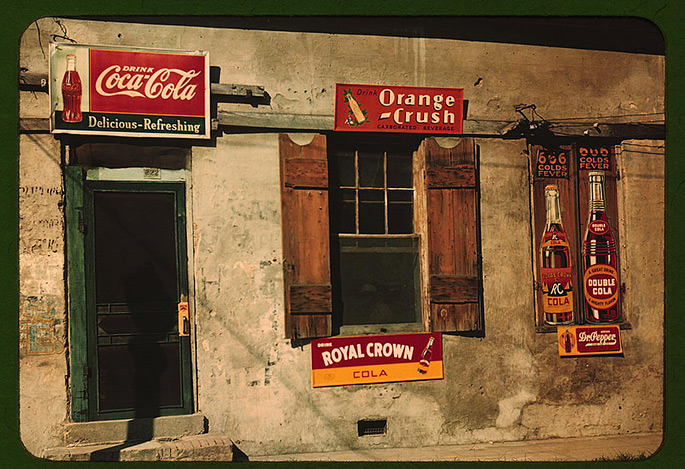
\includegraphics[width=.75\textwidth]{cola-public-domain-photo-p} %{CS0031}
    \caption{Coca-Cola Werbung 1940 \cite{CocaCola1940}.}
    \label{fig:CocaCola}
\end{figure}


\section{Let Them Float!}

Placing figures and tables is one of the most difficult tasks in typesetting
because they usually take up a lot of space and often cannot be placed on the
current page in the running text. These elements must therefore be moved to a
suitable place on subsequent pages, which is very tedious to do manually (but
necessary in \emph{Word}, for example).

When positioning these elements, an attempt is made, on the one hand, to
leave as little empty space as possible in the text flow and, on the other
hand, not to move the figures and tables too far away from the original text
passage. In \latex, this works largely automatically by treating figures,
tables and the like as "floating bodies".

The idea that illustrations, for example, will hardly ever fit exactly in the
desired position and possibly not even on the same page may appear strange or
even frightening for many beginners. Nevertheless, for the time being \latex\
should confidently be left to do this work and the author should \emph{not}
manually intervene! Only when the complete document "stands" and the
automatic placement still appears unsatisfactory, interventions in
\emph{individual} situations are justified.%
\footnote{By adding specific placement instructions (see
\cite[p.~39]{Oetiker2021}).}


\section{Captions}

For figures, the caption is usually placed at the \emph{bottom}, while for
tables---depending on the adopted convention---\emph{above} (as in this
document), but sometimes also at the \emph{bottom}. In \latex\ numbering of
figures is also done automatically, as well as the entry into the (optional)
list of figures at the end of the document.%
\footnote{A separate list of figures at the end of the document is easy to
create, but it is unnecessary in a thesis (and everywhere else, actually).
It should therefore be omitted. However, if your advisor insists on it, you can
find instructions on how to add it to your document in the wiki of the
\texttt{hagenberg-thesis} GitHub repository.}

Captions are marked in \latex using the \verb!\label{}! statement, which must
immediately follow the \verb!\caption{}! statement:
%
\begin{LaTeXCode}[numbers=none]
\begin{figure}
    \centering
    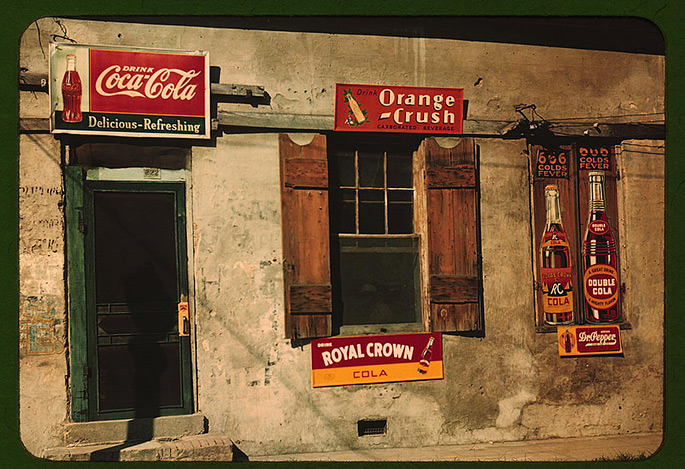
\includegraphics[width=.95\textwidth]{cola-public-domain-photo-p}
    \caption{Coca-Cola Werbung 1940 \cite{CocaCola1940}.}
    \label{fig:CocaCola}
\end{figure}
\end{LaTeXCode}
%
The \emph{name} of the label (\texttt{fig:CocaCola}) can be chosen
arbitrarily. The specific tag "\texttt{fig:}" is (as mentioned in Section
\ref{sec:cross-references}) just a useful aid to better distinguish different
label types when writing.

The length of the captions can be very different. Depending on the
application and style, sometimes a very short caption
(Figure~\ref{fig:CocaCola}) or a longer one (Figure~\ref{fig:ibm360}) results.
Note how short captions are \emph{centered} while long captions use
\emph{justified} formatting (\latex does this automatically). Captions should
\emph{always} end with a period.%
\footnote{Interestingly, some instructions call for the exact opposite,
    supposedly because with classic lead type the final dots are often
    "broken away" in printing. One can believe that or not, but it certainly
    does not matter in digital printing.}

\begin{figure}
    \centering
    \fbox{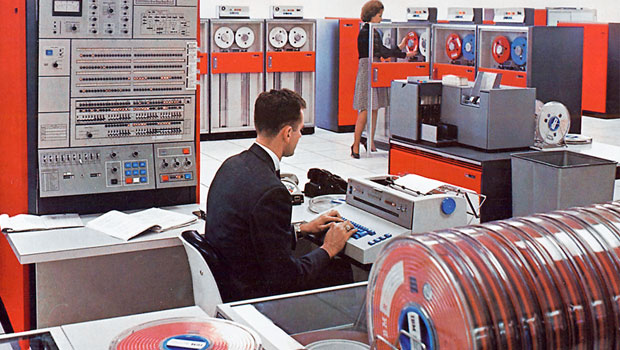
\includegraphics[width=.75\textwidth]{ibm-360-color}}
    \caption{Example of a long caption text. \textsc{Univac} launched the
    Model 751, the first high-performance computer with semiconductor memory,
        in 1961. More than fifty of these computers were sold in the U.S.A.\
        in the first year of production, primarily to military agencies,
        insurance companies, and major banks. It was replaced two years later
        by the Model 820, developed in cooperation with \textsc{Sperry}. This
        may sound plausible, but it is complete nonsense, and the picture
        actually shows a System/360 mainframe computer from IBM. Image
        source~\cite{IBM360}.}
    \label{fig:ibm360}
\end{figure}


\section{Figures}

For the inclusion of graphics in \latex the use of the
standard package \texttt{graphicx} \cite{Carlisle2021} is recommended
(automatically loaded by the \texttt{hagenberg-thesis} package).
With the current workflow (using \texttt{pdflatex}) images and graphics
can only be included in the following formats:
%
\begin{itemize}
    \item PNG: for gray, B/W and color raster images (preferred),
    \item JPEG: for photographs (if not otherwise available),
    \item PDF: for vector graphics (illustrations, line drawings \etc).
\end{itemize}
%
For raster images, PNG should be used if possible, because the images it
contains are compressed losslessly and therefore do not have any visible
compression artifacts. In contrast, JPEG should only be used if the original
material (photo) is already available in this format.


\subsection{Where Are Graphic Files Located?}

Images and graphics are usually stored in a subdirectory (or several
subdirectories), in the case of this document in \nolinkurl{images/}. This is
done by the following statement at the beginning of the main document
\nolinkurl{main.tex} (see also Appendix \ref{app:latex}):
%
\begin{GenericCode}[numbers=none]
\graphicspath{{images/}}
\end{GenericCode}
%
The path \texttt{graphicspath} (relative to the main document) can be changed
at any time within the document, which is quite useful if, \eg, the graphics
of individual chapters are to be stored separately in corresponding directories.


\subsection{Adjusting Picture Size}

The \emph{size} of the printed picture can be controlled by specifying a
certain width or height or a scaling factor, \eg:
%
\begin{GenericCode}[numbers=none]
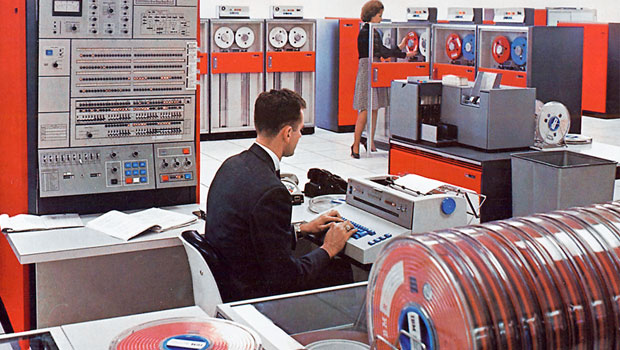
\includegraphics[width=.85\textwidth]{ibm-360-color}
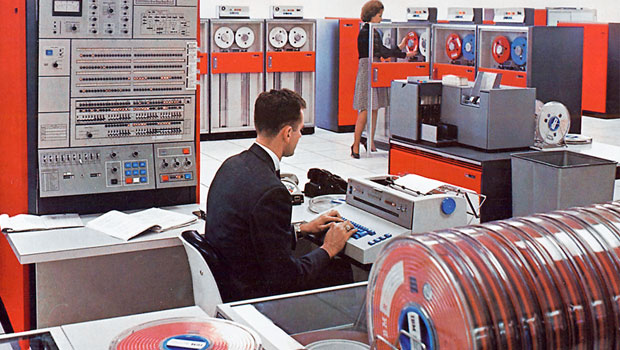
\includegraphics[scale=1.5]{ibm-360-color}
\end{GenericCode}
%
Note that file extensions need not be explicitly specified.
This is particularly convenient when multiple workflows with different file
types are used.


\subsection{Framing Graphics}

The macro \verb!\fbox{...}! can optionally be used to create a thin frame
around the graphic, for example:
%
\begin{GenericCode}[numbers=none]
\fbox{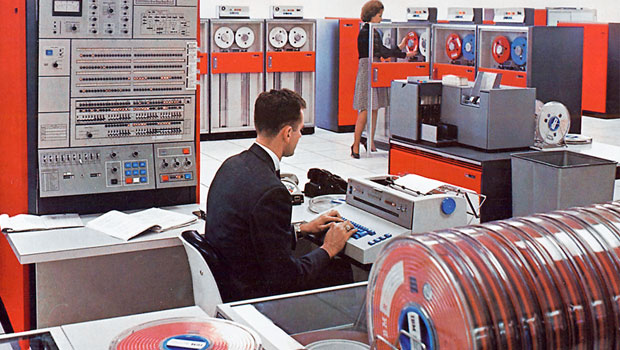
\includegraphics[height=50mm]{ibm-360-color}}
\end{GenericCode}
%
This is usually only necessary for raster images, especially if they are very
bright towards the edge and would not be distinguishable from the background
without a frame.

\subsection{Raster (Pixel) Praphics}

In general, raster images should be prepared in advance so that they lose as
little quality as possible when printed later. It is therefore advisable to
set the image size (resolution) correctly in advance (\eg\ with
\emph{Photoshop}). Common resolutions related to the final image size are:
%
\begin{itemize}
    \item color and gray scale images: 150--300 dpi,
    \item binary (black/white) images: 300--600 dpi.
\end{itemize}
%
A much higher resolution does not make sense due to the screening required in
laser printing, even with 1200 dpi printers. Especially \emph{screen\-shots}
should not be displayed too small, otherwise they are hard to read (max.\ 200
dpi, better 150 dpi). Consider that the work should still be legible in all
details even as a photocopy.

\subsubsection{Careful With JPEG!}

As a rule, images intended for use in print documents should never be saved
using lossy compression methods. In particular, the use of JPEG should be
avoided if possible, even if it makes many files much smaller. The exception
is when the original data is only available in JPEG and has not been edited
or resized for embedding. Otherwise, PNG should always be used.

Often color screenshots are subjected to JPEG compression, although its
devastating consequences should be visible to anyone (see
Figure~\ref{fig:jpeg-bungle}).%
\footnote{The JPEG process is designed for \emph{natural} photos and should
only be used for these.}

\begin{figure}
    \centering\small
    \begin{tabular}{@{}cc@{}}
        \fbox{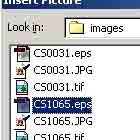
\includegraphics[width=0.475\textwidth]{screenshot-dirty}} &
        % JPEG file
        \fbox{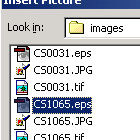
\includegraphics[width=0.475\textwidth]{screenshot-clean}} \\
        % PNG file
        (a) JPEG & (b) PNG
    \end{tabular}
    \caption{Typical JPEG bungle.
    Screenshots and similar raster images available as originals should
    \emph{never} be compressed with JPEG for print documents.
    The result~(a) not only looks dirty compared to the uncompressed
    original~(b), but may also become illegible in print.}
    \label{fig:jpeg-bungle}
\end{figure}

\subsection{Vector (Line) Graphics}

For illustrations and schematic diagrams (\zB flowcharts, entity-relationship
diagrams or other structural representations), vector graphics (PDF) should
always be used. Rasterized graphics, as they are usually available as GIF or
PNG files on web pages, have no place in a print document; if necessary they
must be re-drawn with an appropriate vector graphics tool (of course not
without referencing the original source).

In this case, PDF is really the only choice, being a universal and
standardized container format for many other applications. A suitable
graphics program, \eg, \emph{Adobe Illustrator} or \emph{Inkscape}, is
required to create PDF vector graphics. Note that some popular tools do not
support direct export of PDF files or generate unclean files. Before deciding
on a particular drawing software, this should be tried out in case of doubt.
If everything else fails, PDFs can also be generated by most printer drivers.

\subsubsection{Font Embedding in Graphics}

The rendering of text elements depends on the fonts installed on the computer
(or printer) and the form of font embedding in the source document. Correct
display on the screen of your computer does not mean that the same document
will be displayed exactly the same way on another computer or printer. This
consideration is particularly important when print documents are made
available online. Therefore, make sure that the fonts used in your graphics
appear exactly as intended in the printout (see also Section
\ref{sec:TexFontsInGraphics}).

\subsubsection{Stroke Widths -- Avoid \emph{Hairlines}!}

In graphics programs such as \emph{Illustrator} and \emph{Inkscape}, which
are essentially based on PDF or SVG functionality, it is possible to define
lines in terms of their thickness as "hairlines". This should produce "as
thin as possible" lines in the output. The result depends exclusively on the
respective printer and is therefore hardly predictable. \emph{Conclusion:}
Avoid hairlines and always use concrete line widths ($\geq 0.25\,
\mathrm{pt}$) instead!

\subsection{Using \tex\ Fonts in Graphics}
\label{sec:TexFontsInGraphics}

As a general rule, fonts used in graphics should match the typography of the
main text as closely as possible. An interesting tool for this is \emph{Ipe
Extensible Drawing Editor},%
\footnote{\url{https://ipe.otfried.org/}}
a drawing program that generates text in graphics directly with \latex\
(including mathematical expressions) and uses PDF as its native file format.
For images created with other external graphics programs, you can use at
least \emph{similarly} looking fonts (like \emph{Times-Roman} or
\emph{Garamond}). However, it is also possible to use the
\emph{Computer-Modern} (CM) font family from {\tex}/{\latex} directly to
generate graphics. Some ports of CM are available as \emph{TrueType} fonts,
which can also be used in conventional graphics programs under \emph{Windows}
and \emph{macOS}:
%
\begin{itemize}
    \item
    Recommendable is the "BaKoMa Fonts Collection",%
    \footnote{\url{http://ctan.org/pkg/bakoma-fonts}}
    which contains (beside the CM standard fonts) also the mathematical fonts
    of the
    AMS family.
    \item
    Another option are the "LM-Roman" Open-Type fonts,%
    \footnote{\url{http://www.gust.org.pl/projects/e-foundry/latin-modern}}
    which were specifically developed for use in the \latex environment.
    They are also part of the standard \latex distributions, such as MikTeX.
    These fonts include dedicated glyphs for "umlauts" and are therefore well
    suited for German texts as well.
\end{itemize}
%
Of course, these fonts must first be installed on your computer before 
you can use them.

\subsection{Grapics With \latex Overlays (Using \texttt{overpic})}
\label{sec:GraphicOverlays}

Sometimes it is necessary to overlay an existing image or graphic with
\latex's own (vector) elements, \eg, for markers or labels. A typical example
is shown in Figure~\ref{fig:overpic-example} where a PDF graphic created with
\emph{Mathematica} is annotated with mathematical text elements. This is
accomplished using the \texttt{overpic} package, where the underlying graphic
is not imported with \verb!\includegraphics! but \verb!\begin{overpic}!
\ldots \verb!\end{overpic}!, with a similar syntax:
%
\begin{LaTeXCode}[numbers=none]
\begin{overpic}[width=0.85\textwidth]{mathematica-example}
    \put(101,14){$x$}%
    \put(4,31){$f(x)$}%
    \put(29.5,28){\line(1,1){2}}%
    ...
\end{overpic}
\end{LaTeXCode}

\begin{figure}
    \centering\small
    \vspace*{3mm}
    \begin{overpic}[width=0.85\textwidth]{mathematica-example}
        \put(101,14){$x$}%
        \put(4,31){$f(x)$}%
        \put(29.5,28){\line(1,1){2}}%
        {\color{green!70!black}\put(29.5,28){\circle*{2.0}}}%
        \put(32,30){$\cos(\frac{7}{3} x)$}%
        \put(59,28){\line(1,1){2}}%
        {\color{blue!70!black}\put(59,28){\circle*{2.0}}}%
        \put(61.5,30){$\cos(x)$}%
    \end{overpic}
    \caption{Example of using the \texttt{overpic} package to insert \latex
    elements over an imported graphic. In this case, the mathematical
    elements $x$, $f(x)$, $\cos(x)$ and $\smash{\cos(\frac{7}{3} x)}$ as well
    as two diagonal straight lines and filled (colored) circles were inserted
    . All this is drawn on top of a vector graphic imported from file
    \texttt{mathematica-example.pdf}.}
    \label{fig:overpic-example}
\end{figure}

The \texttt{overpic} environment also forms a \texttt{picture} environment%
\footnote{\url{https://www.overleaf.com/learn/latex/Picture_environment}}
where \latex drawing instructions (such as \verb!\put! and the like) can be
placed, as shown in Figure~\ref{fig:overpic-example}.%
\footnote{The default drawing instructions in \latex are quite restrictive,
so the \texttt{pict2e} package is additionally used (see
\url{https://ctan.org/pkg/pict2e}).}
The $x/y$ positions are specified as a percentage of the image width. Further
details can be found in the source code.

\subsection{Figures With Multiple Elements}

If multiple images or graphics are combined into one figure, a common caption
is typically used, as shown in Figure~\ref{fig:Bearings}. In the main text, a
reference to a particular part of the figure, such as the single-row roller
bearing in Figure~\ref{fig:Bearings}\,(c), could look like this:
%
\begin{LaTeXCode}[numbers=none]
... Figure~\ref{fig:Bearings} (c) ...
\end{LaTeXCode}

\subsection{Source Citations in Captions}
\label{sec:SourceCitationsInCaptions}

If images, graphics or tables from other sources are used, then their origin
must be made clear in any case, and preferably directly in the caption. For
example, if an illustration from a book or other citable publication is used,
then it should be included in the bibliography and cited as usual with
\verb!\cite{..}! as demonstrated in Fig.\ \ref{fig:Bearings}. Further details
on this type of source citation can be found in Chapter~\ref{cha:Literature}
(esp.\ Section~\ref{sec:category-online}).

\begin{figure}
    \centering\small
    \begin{tabular}{@{}c@{\hspace{12mm}}c@{}} % mittlerer Abstand = 12mm
        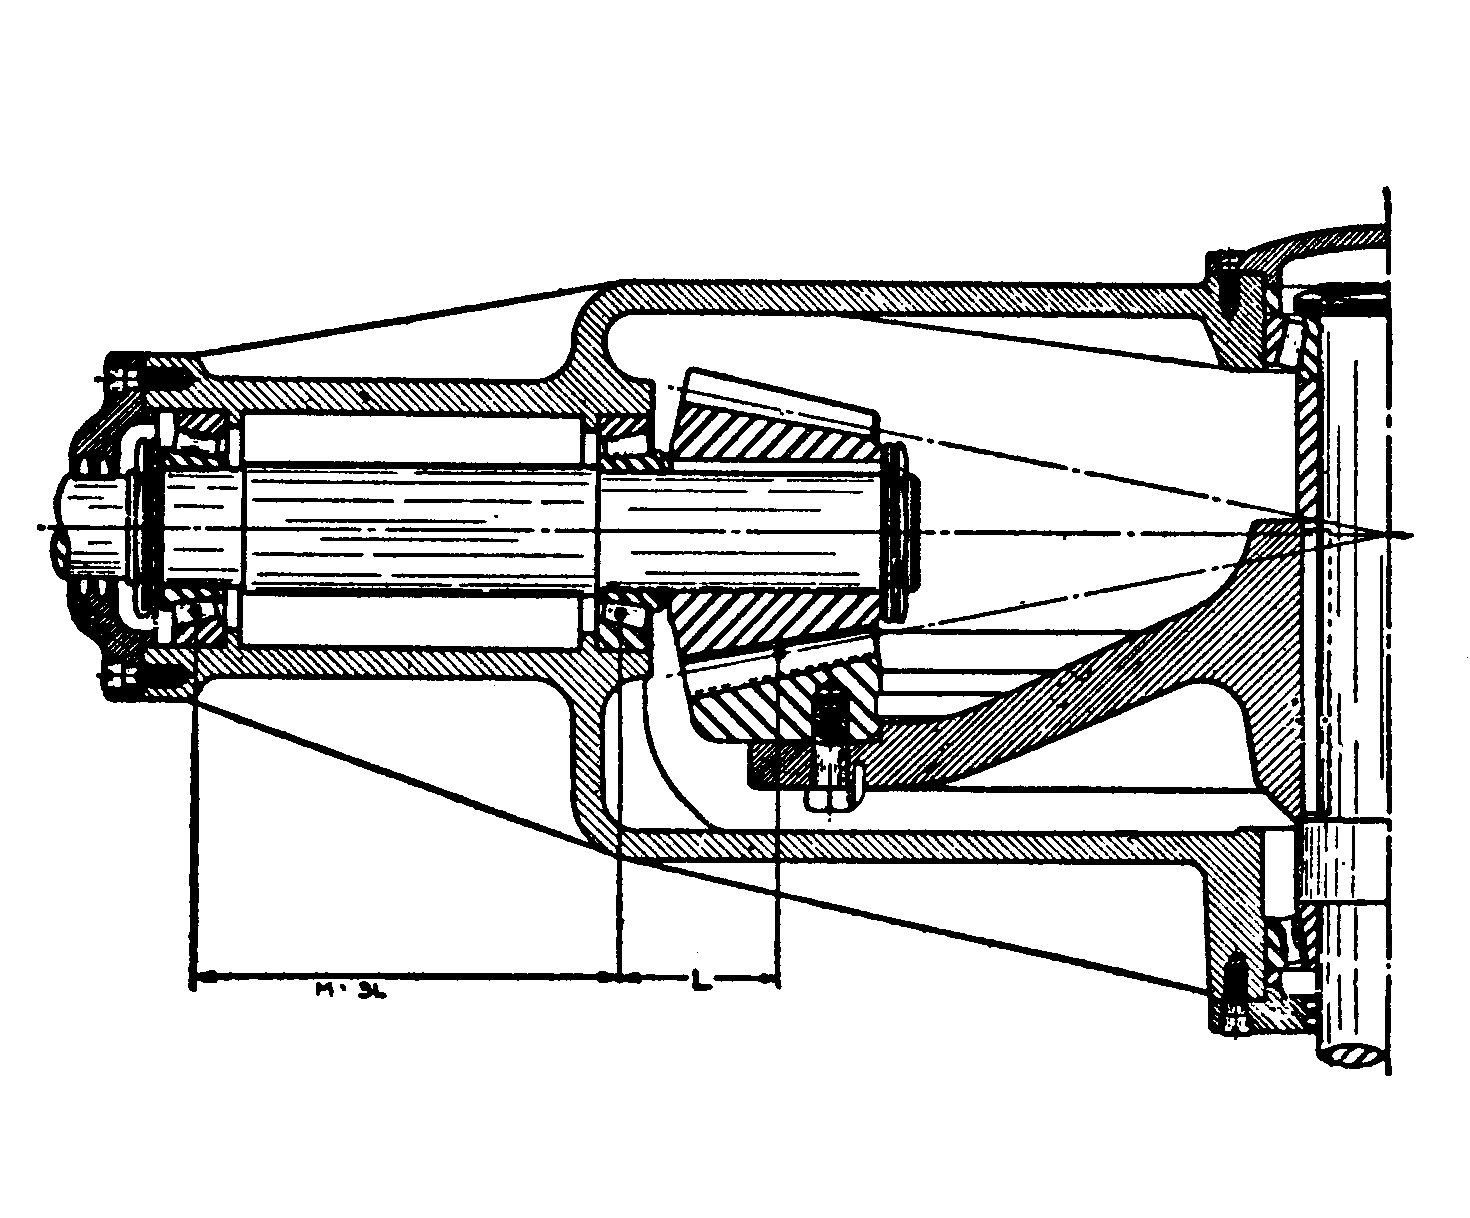
\includegraphics[width=.45\textwidth]{overhang-mounting} &
        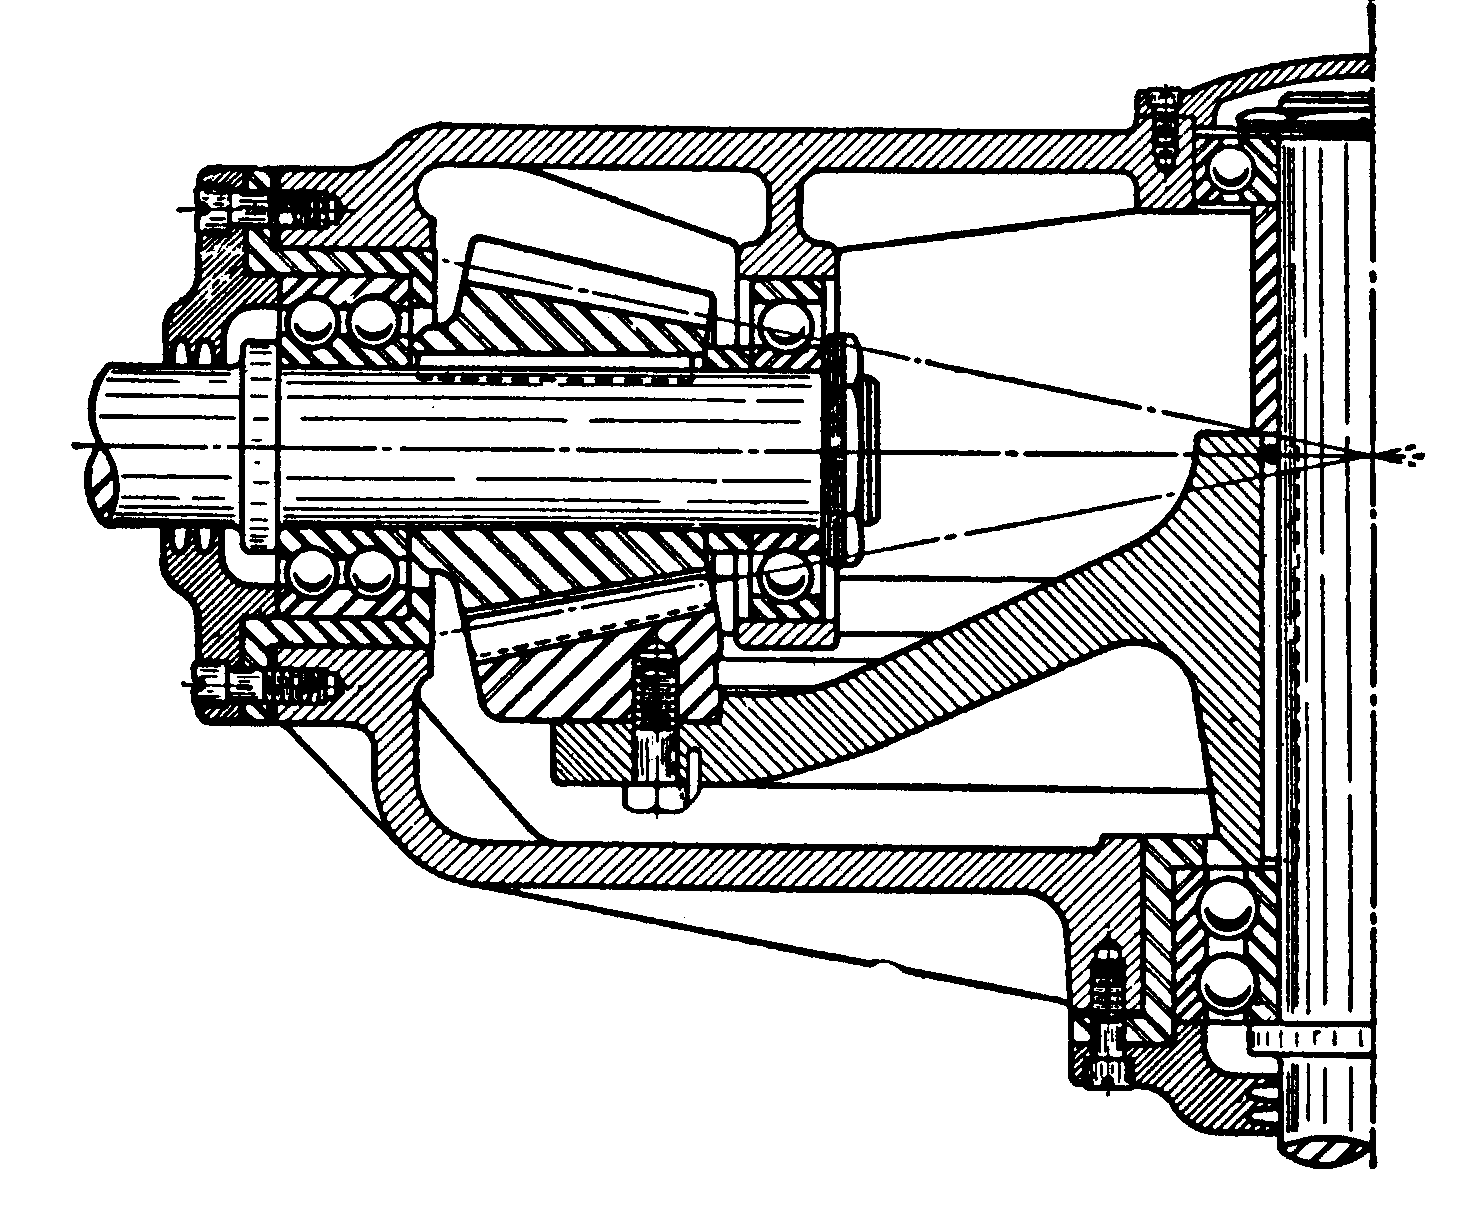
\includegraphics[width=.45\textwidth]{straddle-mounting}
        \\
        (a) & (b)
        \\[4pt]    %vertical extra spacing (4 points)
        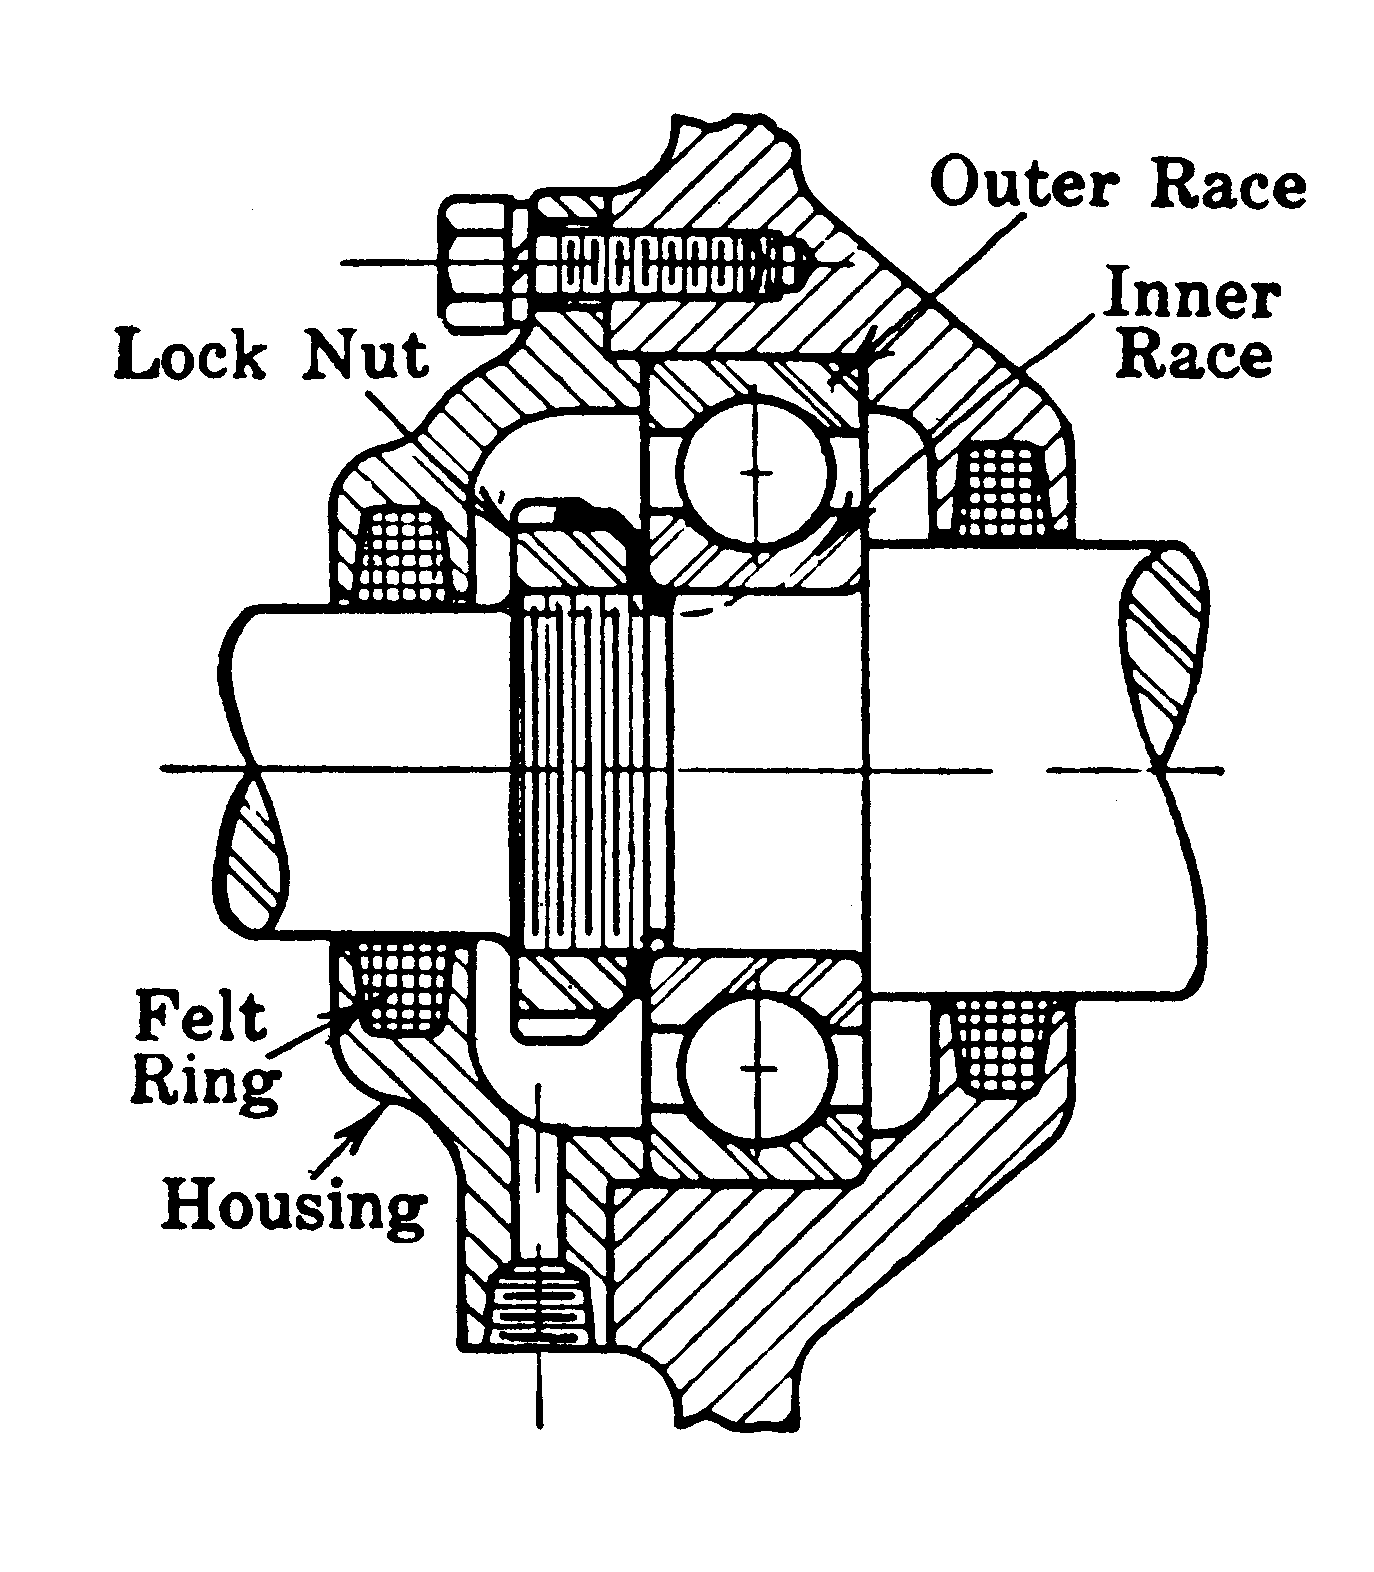
\includegraphics[width=.45\textwidth]{ball-bearing-1} &
        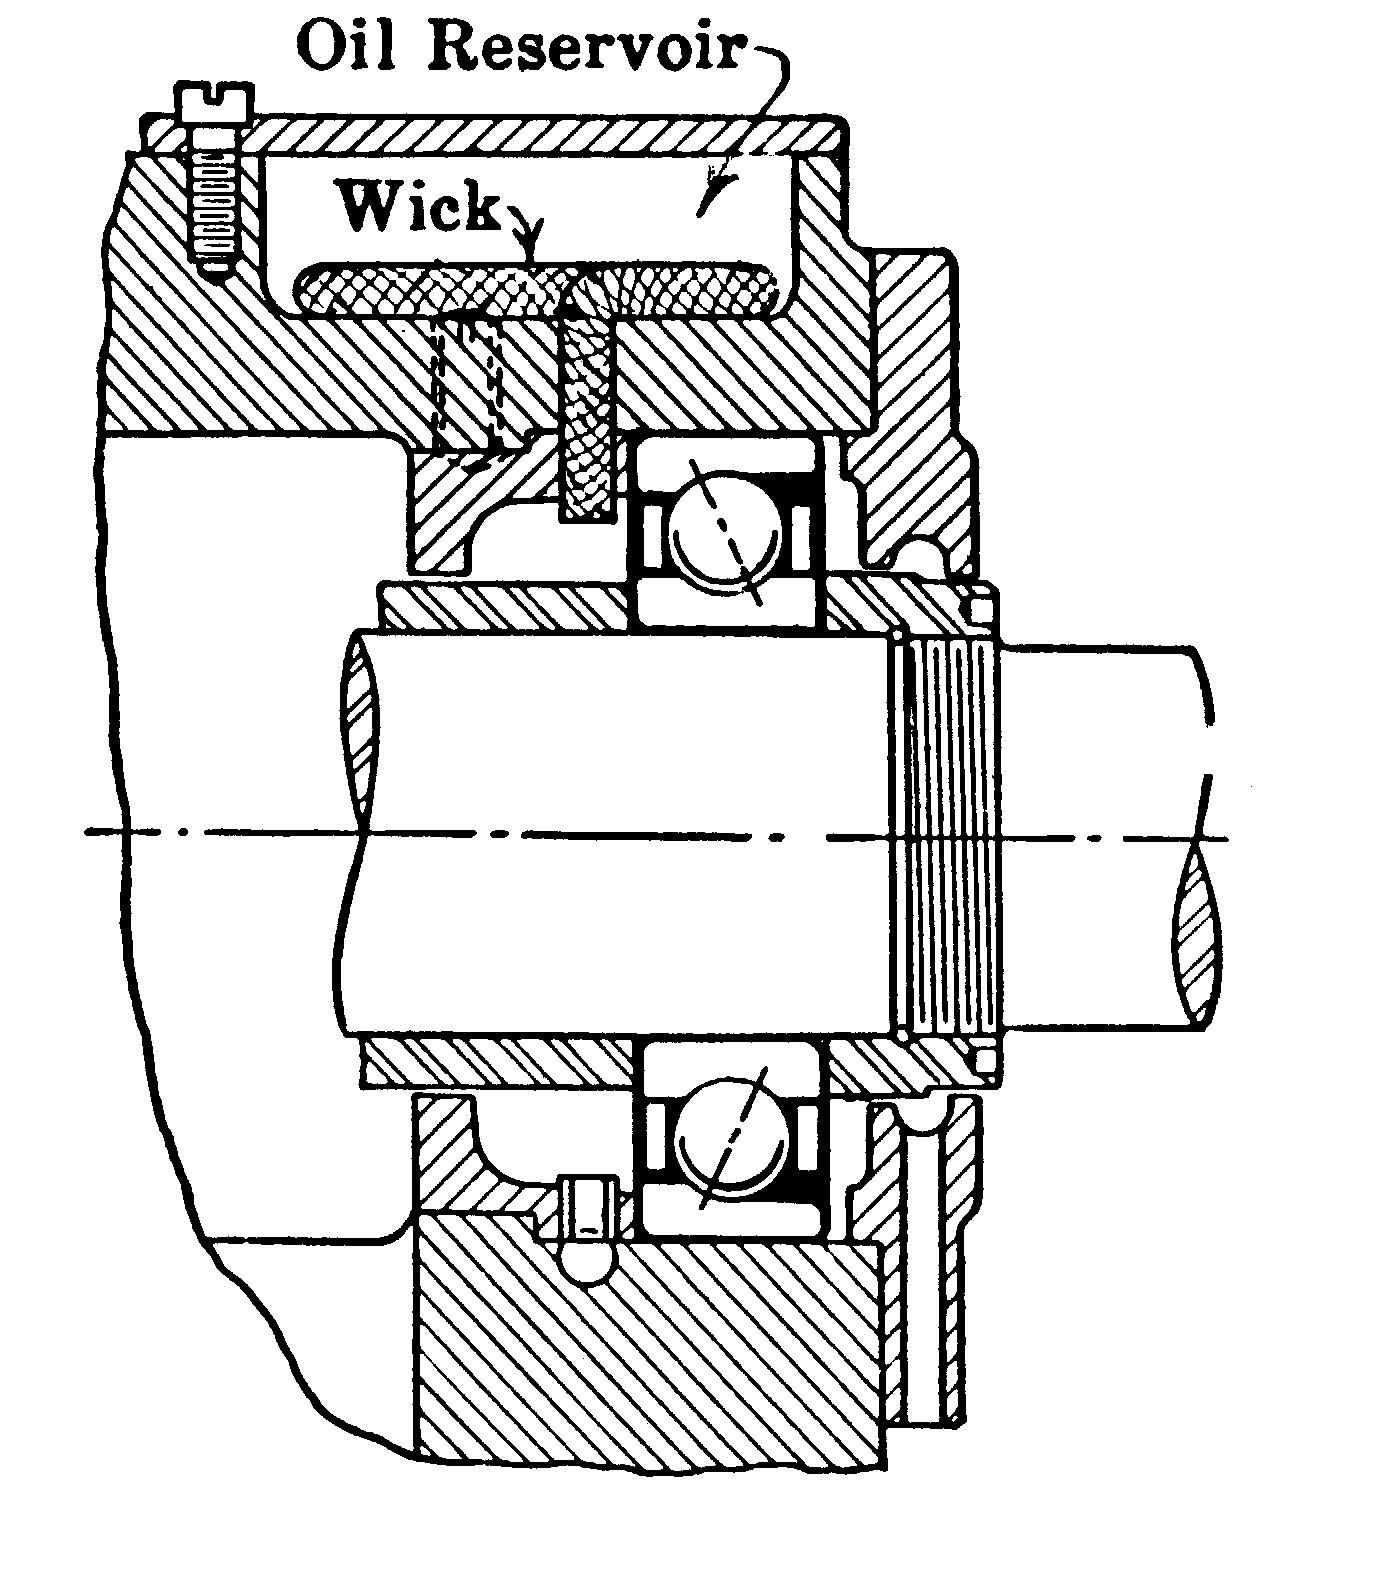
\includegraphics[width=.45\textwidth]{ball-bearing-2}
        \\
        (c) & (d)
    \end{tabular}
%
\caption{Various machine elements in an illustration with multiple elements.
\emph{Overhang mounting}~(a), \emph{straddle mounting}~(b), single row roller
bearing~(c), lubrication of roller bearings~(d). This figure uses an ordinary
table (\texttt{tabular}) with 2 columns and 4 rows (details can be found in
the source code). Image source~\cite{Faires1934}.}
\label{fig:Bearings}
\end{figure}


\section{Tables}
\label{sec:Tables}

Tables are often used to present numerical relationships, test results, etc.\
in a clear form. A simple example is Table~\ref{tab:programming-languages},
the associated \latex source can be found in 
Program~\ref{prog:programming-languages-source}.

As arguments of the \texttt{tabular} environment the alignments of the
individual columns are specified. The number of arguments thus determines the
number of columns. Valid items are \texttt{l} for left-aligned, \texttt{c}
for centered, and \texttt{r} for right-aligned. The column width results from
the length of the contents, there are no automatic line breaks. To set the
width and thus create automatic line wraps, \verb|p{width}| (paragraph mode)
is used, where \texttt{width} is a valid length specification (see
\cite{WikibooksLaTeXLengths2018} for details). The \verb|@{}| items remove
the (usually unwanted) margin at the left and right table borders.

\begin{table}
    \caption{Programming languages at a glance.}
    \label{tab:programming-languages}
    \centering
    \setlength{\tabcolsep}{10pt} 				% separator between columns (standard = 6pt)
    \renewcommand{\arraystretch}{1.25}	% vertical stretch factor (standard = 1.0)
    \begin{tabular}{@{}llll@{}}
        \toprule
        Language   & Type        & Typical Use      & Standards          \\
        \midrule
        C++        & Compiled    & Applications     & ISO/IEC 14882:2020 \\
        COBOL      & Compiled    & Business         & ISO/IEC 1989:2014  \\
        JavaScript & Interpreted & Web              & ECMA-262           \\
        Python     & Interpreted & Machine Learning & PEPs               \\
        \bottomrule
    \end{tabular}
\end{table}

\begin{program}
% place caption consistently either at the top or bottom:
    \caption{\latex\ source code for Table \ref{tab:programming-languages}.
    The generation of the displayed listing itself is described in
    Section~\ref{sec:program-texts}.}
    \label{prog:programming-languages-source}
%
\begin{LaTeXCode}[numbers=none]
\begin{table}
    \caption{Programming languages at a glance.}
    \label{tab:programming-languages}
    \centering
    \setlength{\tabcolsep}{10pt} % separator between columns (standard = 6pt)
    \renewcommand{\arraystretch}{1.25} % vertical stretch factor (standard = 1.0)
    \begin{tabular}{@{}llll@{}}
        \toprule
        Language   & Type        & Typical Use      & Standards          \\
        \midrule
        C++        & Compiled    & Applications     & ISO/IEC 14882:2020 \\
        COBOL      & Compiled    & Business         & ISO/IEC 1989:2014  \\
        JavaScript & Interpreted & Web              & ECMA-262           \\
        Python     & Interpreted & Machine Learning & PEPs               \\
        \bottomrule
    \end{tabular}
\end{table}
\end{LaTeXCode}
%
\end{program}

The demand for an attractive appearance of tables has increased noticeably in
recent years. For example, many authors and publishers using \latex now
follow some simple design guidelines for tables \cite{Fear2020}, of which
particularly the first two determine their basic layout:

\begin{enumerate}
    \item Never use vertical lines.
    \item Never use double lines.
    \item Place units in the column header (not in the table content area).
    \item A decimal separator is always preceded by a digit; thus write
    "$0{,}1$" not just "${,}1$".
\end{enumerate}


The \latex package \texttt{booktabs} makes it easy to meet these requirements
Within the \texttt{tabular} environment (which defines the actual table), the
number of columns---preferably set left-justified (\texttt{l}
specifiers)--- are defined first. \verb|\toprule| marks the beginning of the
table, followed by the header, which is terminated by \verb|\midrule|. This is
followed by the lines with the table contents. Using \verb|\bottomrule| the
table is closed with another horizontal line. \verb|\midrule| calls can also
occur more often to divide the table. If horizontal lines are needed that should
not span all columns, \verb|\cmidrule| can be used.

\subsection{Long Texts in Table Columns}

Sometimes it is necessary to fit relatively large amounts of text into narrow
columns in tables, as in Table \ref{tab:synthesis-techniques}. In this case,
it makes sense to go without justification and at the same time relax the
strict hyphenation rules. Details can be found in the corresponding \latex
source text.


%--------------------------------------------------------------------------------
% Table with narrow columns
%--------------------------------------------------------------------------------
\begin{table}
    \caption{Example of a table with multiline text in narrow columns.
    Here the columns are too narrow for justification, so left alignment
        ("ragged-right") is used.}
    \label{tab:synthesis-techniques}
    \centering
    \newcommand{\RR}{\rightskip=0pt plus1em \spaceskip=.3333em \xspaceskip=.5em\relax}
    \renewcommand{\arraystretch}{1.20}
    \small
    \begin{english}
        \begin{tabular}{@{}p{0.2\textwidth}lp{0.3\textwidth}p{0.2\textwidth}@{}}
            \toprule
            Method & Implem. & Features & Status \\
            \midrule
            {\RR polygon shading} &
            SW/HW &
                {\RR flat-shaded polygons} &
            \\
            {\RR flat shading with z-buffer} &
            SW/HW &
                {\RR depth values} &
            \\
            {\RR goraud shading with z-buffer} &
            SW/HW &
                {\RR smooth shading, simple fog, point light sources} &
                {\RR SGI entry models} \\
            {\RR phong shading with z-buffer} &
            SW/HW &
                {\RR highlights} &
            \\
            {\RR texture mapping with z-buffer} &
            SW/HW &
                {\RR surface textures, simple shadows} &
                {\RR SGI high end, flight simulators} \\
            \bottomrule
        \end{tabular}
    \end{english}
\end{table}


\subsection{Multipage Tables}

Often tabular information needs more than one page. Here the float-element
created by the \texttt{table} environment becomes a problem, because it
prevents breaks across multiple pages. To allow page breaks \emph{within}
tables, the \texttt{longtable} package can be used.%
\footnote{%
\url{http://mirrors.ctan.org/macros/latex/required/tools/longtable.pdf}}
It replaces the \texttt{tabular} environment and does not require a
surrounding \texttt{table} environment.%
\footnote{Note that a \texttt{longtable} is \emph{no} float element but 
always gets inserted at the current text position. This may lead to large
empty blocks if the table header and/or the first table row do not fit onto
the current page.}

The table definition is largely the same as shown in Program
\ref{prog:programming-languages-source}. Only the commands \verb|\endhead|
and \verb|\endfoot| are added. They outline the head and footer areas to be
repeated on each page. If these should be different for the header on the
first page and the footer on the last page, \verb|\endfirsthead| and
\verb|\endlastfoot| are used.

Table \ref{tab:LongtableDemo} shows a concrete example for using 
\texttt{longtable}. A specific header is assigned to the first page, 
defining the main caption text and the associated label.
The following pages show an abbreviated header ("\emph{continued}") with the
\emph{same} table number, which is only defined once in the main header. 
If horizontal and vertical spacing are to be modified, these statements must
be placed \emph{before} the beginning of the table and enclosed with
\verb|{|\ldots\verb|}| or \verb|\begin{block}| \ldots \verb|\end{block}|%
\footnote{The (dummy) "\texttt{block}" environment is defined in 
\texttt{hgb.sty}. It does nothing but provides a limited scope for
temporarily setting (and automatically resetting) \latex\ variables.}
to restrict their scope. Consult the source code of this document for
additional details.

\begin{block}										 % 'block' environment is defined in hgb.sty
\setlength{\tabcolsep}{10pt}     % separator between columns (standard = 6pt)
\renewcommand{\arraystretch}{1.50} % vertical stretch factor (standard = 1.0)
\begin{longtable}{@{}lp{0.23\textwidth}@{}}
		% -------------------------- first header ----------------------------
    \caption{A long table (using \texttt{longtable}) that breaks over two pages. 
		Note that different table headers are defined for the first page and
		subsequent pages and the associated label is only assigned once 
		(referring to \emph{this} page).} 
		\label{tab:LongtableDemo}																						 \\
    \toprule
    First Column            & Second Column                              \\
    \midrule
		\endfirsthead
		% ---------------------- subsequent headers ---------------------------
		\caption*{\textbf{Table \getcurrentlabel} (\emph{continued})}				 \\
    \toprule
    First Column            & Second Column                              \\
    \midrule
		\endhead
		% --------------------------------------------------------------------
    The column on the right contains a lot of text. &
    There is a lot of text in this column, which creates a long column.
    Here, too, it can make sense to set the content left-aligned. However,
    \texttt{longtable} does not wrap lines in such columns, only between
    individual lines. \\
    More lines follow here. & This content serves only as a placeholder. \\
    More lines follow here. & This content serves only as a placeholder. \\
    More lines follow here. & This content serves only as a placeholder. \\
    More lines follow here. & This content serves only as a placeholder. \\
    More lines follow here. & This content serves only as a placeholder. \\
    More lines follow here. & This content serves only as a placeholder. \\
    More lines follow here. & This content serves only as a placeholder. \\
    More lines follow here. & This content serves only as a placeholder. \\
    More lines follow here. & This content serves only as a placeholder. \\
		More lines follow here. & This content serves only as a placeholder. \\
    More lines follow here. & This content serves only as a placeholder. \\
    More lines follow here. & This content serves only as a placeholder. \\
    More lines follow here. & This content serves only as a placeholder. \\
    More lines follow here. & This content serves only as a placeholder. \\
    More lines follow here. & This content serves only as a placeholder. \\
    More lines follow here. & This content serves only as a placeholder. \\
    More lines follow here. & This content serves only as a placeholder. \\
    More lines follow here. & This content serves only as a placeholder. \\
    \bottomrule
\end{longtable}
\end{block}

%{\setlength{\tabcolsep}{10pt} % separator between columns (standard = 6pt)
%\def\arraystretch{1.50}      % vertical stretch factor (standard = 1.0)
%\begin{longtable}{@{}lp{0.23\textwidth}@{}}
    %\caption{A long table that potentially breaks over two pages.} \\
    %\toprule
    %First Column            & Second Column                              \\
    %\midrule\endhead
    %\label{tab:LongtableDemo}
    %The column on the right contains a lot of text. &
    %There is a lot of text in this column, which creates a long column.
    %Here, too, it can make sense to set the content left-aligned. However,
    %\texttt{longtable} does not wrap lines in such columns, only between
    %individual lines. \\
    %More lines follow here. & This content serves only as a placeholder. \\
    %More lines follow here. & This content serves only as a placeholder. \\
    %More lines follow here. & This content serves only as a placeholder. \\
    %More lines follow here. & This content serves only as a placeholder. \\
    %More lines follow here. & This content serves only as a placeholder. \\
    %More lines follow here. & This content serves only as a placeholder. \\
    %More lines follow here. & This content serves only as a placeholder. \\
    %More lines follow here. & This content serves only as a placeholder. \\
    %More lines follow here. & This content serves only as a placeholder. \\
    %\bottomrule
%\end{longtable}}


\subsection{Joining Columns and Rows}

To combine several columns in a table into one, the statement
%
\begin{GenericCode}[numbers=none]
\multicolumn{number}{format}{text}
\end{GenericCode}
%
is used. Here \texttt{number} defines the set of columns to be joined.
\texttt{format} specifies the alignment to use analogous to the specification
in \texttt{tabular}-environment and \texttt{text} is the included text.

Analogously, to combine several lines into one, you can use
%
\begin{GenericCode}[numbers=none]
\multirow{number}{width}{text}
\end{GenericCode}
%
Here \texttt{number} represents the number of lines to be joined into one,
\texttt{width} defines the joint column width. The same specifications are
used as in the \texttt{tabular} environment. Additionally, \texttt{*} and
\texttt{=} can be specified. The former sets the width created by the text,
the latter takes the width of the column from the \texttt{tabular}
specification. \texttt{text} is the content to be inserted.

The \verb|multirow| command is placed in the first of the lines to be joined.
The following rows remain empty. Table \ref{tab:multi-column-row-table} shows
a simple example with joined columns and rows.


\begin{table}[htbp]
    \caption{A table with joined columns and rows.}
    \label{tab:multi-column-row-table}
    \centering
    \setlength{\tabcolsep}{10pt} % separator between columns (standard = 6pt)
    \renewcommand{\arraystretch}{1.25}      % vertical stretch factor (standard = 1.0)
    \begin{tabular}{@{}lll@{}}
        \toprule
        Column 1 & \multicolumn{2}{c}{Columns 2--3} \\
        \midrule
        Row 1 &
        \multirow{2}{4cm}{This text extends over two lines.} &
        \multirow{2}{*}{This text too.} \\
        Row 2 & & \\
        \bottomrule
    \end{tabular}
\end{table}


\section{Program Texts}
\label{sec:program-texts}

The inclusion of program texts (source code) is a frequent necessity,
especially of course for work in areas related to computing.

\subsection{Formatting Program Code}
\label{sec:FormattingProgramCode}

There are special packages for \latex\ to display programs which, among other
things, also perform automatic line numbering, in particular the packages
\texttt{listings}%
\footnote{\url{https://ctan.org/pkg/listings}}
and \texttt{listingsutf8}.%
\footnote{\url{https://ctan.org/pkg/listingsutf8}}

\begin{table}
    \caption{Language-specific code environments defined in \nolinkurl{hgb
    .sty}.}
    \label{tab:CodeEnvironments}
    \centering
    \begin{tabular}{@{}lll@{}}
        \toprule
        C (ANSI): & \verb!\begin{CCode}!
        & \verb!...! \verb!\end{CCode}! \\
        C++ (ISO): & \verb!\begin{CppCode}!
        & \verb!...! \verb!\end{CppCode}! \\
        C\#: & \verb!\begin{CsCode}!
        & \verb!...! \verb!\end{CsCode}! \\
        CSS: & \verb!\begin{CssCode}!
        & \verb!...! \verb!\end{CssCode}! \\
        HTML: & \verb!\begin{HtmlCode}!
        & \verb!...! \verb!\end{HtmlCode}! \\
        Java: & \verb!\begin{JavaCode}!
        & \verb!...! \verb!\end{JavaCode}! \\
        JavaScript: & \verb!\begin{JsCode}!
        & \verb!...! \verb!\end{JsCode}! \\
        \latex: & \verb!\begin{LaTeXCode}!
        & \verb!...! \verb!\end{LaTeXCode}! \\
        Objective-C: & \verb!\begin{ObjCCode}!
        & \verb!...! \verb!\end{ObjCCode}! \\
        PHP: & \verb!\begin{PhpCode}!
        & \verb!...! \verb!\end{PhpCode}! \\
        Python: & \verb!\begin{PythonCode}!
        & \verb!...! \verb!\end{PythonCode}! \\
        Swift: & \verb!\begin{SwiftCode}!
        & \verb!...! \verb!\end{SwiftCode}! \\
        XML: & \verb!\begin{XmlCode}!
        & \verb!...! \verb!\end{XmlCode}! \\
        Generic: & \verb!\begin{GenericCode}!
        & \verb!...! \verb!\end{GenericCode}! \\
        \bottomrule
    \end{tabular}
\end{table}

These are also used to implement the language-specific environments listed in
Table~\ref{tab:CodeEnvironments}. Their use is extremely simple, \eg, for
source code in the C programming language one writes
%
\begin{GenericCode}[numbers=none]
\begin{CCode}
    ... 
\end{CCode}
\end{GenericCode}
%
The source code within these environments is interpreted in the respective
programming language, while comments are preserved. These environments can be
used standalone (in the main text) or within float environments (esp.\
\texttt{program}). In the first case, the source text even wraps across page
boundaries. With \verb!/+! \ldots \verb!+/! an escape option to \latex\ is
provided, which is useful for setting labels for referencing individual
program lines, \eg, with
%
\begin{GenericCode}[numbers=none]
int w = ip.getWidth(); /+\label{ExampleCodeLabel}+/
\end{GenericCode}
%
An example with Java is shown in Prog.~\ref{prog:CodeExample}, where the
above label is placed in line \ref{ExampleCodeLabel}. Note that mathematical
text (such as in line \ref{MathInCode} of Prog.~\ref{prog:CodeExample}) can
also be placed inside escaped comments.


\subsubsection{Numbering of the Code Lines}

All code environments listed in Table~\ref{tab:CodeEnvironments} can be used
with optional arguments, which are especially useful to control the line
numbering. In the default case (\ie, without additional specifications), with
%
\begin{LaTeXCode}[numbers=none]
\begin{/+\emph{some}+/Code} ... 
\end{LaTeXCode}
%
all code lines (including blank lines) are continuously numbered starting at
1. For consecutive code segments it is often helpful to let the numbering
continue from the previous section, enabled by specifying the optional argument
\texttt{firstnumber={\obnh}last}:
%
\begin{LaTeXCode}[numbers=none]
\begin{/+\emph{some}+/Code}[firstnumber=last] ... 
\end{LaTeXCode}
%
To disable the numbering of the code lines altogether it is sufficient to
specify the optional argument
\texttt{numbers={\obnh}none}:
%
\begin{LaTeXCode}[numbers=none]
\begin{/+\emph{some}+/Code}[numbers=none] ... 
\end{LaTeXCode}
%
In this case, of course, the use of line labels in the code has no effect.


\subsection{Program Code Placement}

Since source texts can become quite bulky, this task is not always easy to
solve. Depending on the size and the relation to the main text, there are
essentially three ways for including program text:
%
\begin{itemize}
    \item[a)] in the main text for short program pieces,
    \item[b)] as float elements (\texttt{program}) for medium-sized programs
    up to one page, or
    \item[c)] in the Appendix (for long programs).
\end{itemize}


\subsubsection{Program Code in the Main Text}

Short code sequences can be embedded in the running text without further ado,
as long as they are of immediate importance at the given places.
For example, the following (rudimentary) Java method \texttt{extractEmail}
searches for an e-mail address in a given string:
%
\begin{JavaCode}[numbers=none]
static String extractEmail(String line) {
    line = line.trim(); // find the first blank
    int i = line.indexOf(' ');
    if (i > 0)
    return line.substring(i).trim();
    else
    return null;
}
\end{JavaCode}
%
\noindent
This code segment was produced with
%
\begin{LaTeXCode}[numbers=none]
\begin{JavaCode}[numbers=none]
static String extractEmail(String line) {
    line = line.trim(); // find the first blank
    ...
}
\end{JavaCode}
\end{LaTeXCode}
%
(see Section \ref{sec:FormattingProgramCode}). In-line program pieces should be
no more than a few lines long and, if possible, should not be divided by page
breaks.


\subsubsection{Program Code in Float Elements}

Suppose longer code sequences are necessary, which should appear near the
running text. In that case, they should be treated as float elements in the same
way as illustrations and tables. These program texts should not exceed the size
of one page. In an emergency, up to two pages can be packed into consecutive
float elements, each with its own caption. In \texttt{hgb.sty} a float
environment \texttt{program} is defined, which is used analogously to
\texttt{table}:
%
\begin{LaTeXCode}[numbers=none]
\begin{program}
\caption{The title of this piece of program.}
\label{prog:xyz}
\begin{JavaCode}
  class Foo {
    ...
  }
\end{JavaCode}
\end{program}
\end{LaTeXCode}
%
If desired, the caption can also be placed at the bottom (but in any case
consistently and not mixed). Of course, a linear sequence in the final
printed image must not be expected here either, so phrases such as "\ldots\
in the \emph{following} program snippet \ldots" should be avoided and
numerical cross references used instead. See Programs
\ref{prog:programming-languages-source} and \ref{prog:CodeExample} for examples.


\begin{program}
% place caption consistently either at the top or bottom:
\caption{Example of a program listing (Java) as a float element.}
\label{prog:CodeExample}
\begin{JavaCode}
import ij.ImagePlus;
import ij.plugin.filter.PlugInFilter;
import ij.process.ImageProcessor;

public class My_Inverter implements PlugInFilter {
    int agent_velocity;
    String title = ""; // just to test printing of double quotes

    public int setup (String arg, ImagePlus im) {
        return DOES_8G;
    }

    public void run (ImageProcessor ip) {
        int w = ip.getWidth(); /+\label{ExampleCodeLabel}+/
        int h = ip.getHeight();

        /* iterate over all image coordinates */
        for (int u = 0; u < w; u++) {
            for (int v = 0; v < h; v++) {
                int p = ip.getPixel(u, v);
                ip.putPixel(u, v, 255 - p); // invert: /+\smash{$I'(u,v) \leftarrow (255 - I(u,v))$}\label{MathInCode}+/
            }
        }
    }
} // end of class /+My\_Inverter+/
\end{JavaCode}
%
\end{program}

\subsubsection{Program Texts in the Appendix}

For longer program texts, especially if they include complete implementations
and are not directly relevant in any local context, storage in a separate
appendix at the end of the document should be resorted to. For references to
individual details, either short excerpts can be placed in the running text
or appropriate page references can be used. Such an example is the \latex
source code in Appendix \ref{app:latex} (page \pageref{app:latex}).%
\footnote{It is generally questionable if the printed inclusion of 
much implementation code is at all useful for the reader or not better
provided electronically (on physical media or online) and only described
selectively.}


%\chapter[Mathematical Formulas etc.]{Mathematical Formulas, Equations and Algorithms}
\label{cha:Mathematics}


Typesetting mathematical elements is certainly one of the strongest features of
\latex. A distinction is made between mathematical elements in continuous text
and free-standing equations, which are usually numbered consecutively.
Analogous to figures and tables, this makes it easy to cross-reference equations.
Here are only some examples and special topics, much more can be found in 
\cite[Ch.\ 7]{Kopka2003} and~\cite{Voss2014}.


\section{Mathematical Elements in Continuous Text}

Mathematical symbols, expressions, equations, etc.\ are marked in the continuous
text by pairs \verb!$! \ldots \verb!$!. Here is an example:
%
\begin{quote}
	%\item[]
	The near infinity point is at $\bar{a} = f \cdot (f / (K \cdot u_{\max}) + 1)$, 
	so with a lens set to $\infty$, everything is in focus from distance $\bar{a}$ on.
	Focusing the lens to the distance $\bar{a}$ (\ie, $a_0 = \bar{a}$), everything
	in the range $[\frac{\bar{a}}{2}, \infty]$ will be in focus.
\end{quote}
%
It is important to ensure that the height of the individual math items in the text
does not become too large.

\subsubsection{Common Mistakes}

In continuous text, simple variables are often typeset with plain text,
\ie, without using correct mathematical symbols, as in "X-axis" instead of 
"$X$-axis" (\verb!$X$-axis!).


\subsubsection{Mathematical Fonts}

\latex\ uses slightly different fonts for regular text and in math mode.
The following basic math fonts are available:
%
\begin{quote}
    \begin{tabular}{lcl}
        $\mathrm{Roman}$      & & \verb!$\mathrm{Roman}$!,      \\
				$\mathit{Italic}$     & & \verb!$\mathit{Italic}$!,      \\
				$\mathbf{Bold}$     	& & \verb!$\mathit{Bold}$!,      \\
        $\mathsf{Sans Serif}$ & & \verb!$\mathsf{Sans Serif}$!, \\
        $\mathtt{Typewriter}$ & & \verb!$\mathttt{Typewriter}$!, \\
				$\mathcal{CALLIGRAPHIC}$ & & \verb!$\mathcal{CALLIGRAPHIC}$!,\\
				$\mathbb{BLACKBOARD}$ & & \verb!$\mathbb{BLACKBOARD}$!,\\
				$\mathfrak{Fraktur}$ & & \verb!$\mathfrak{Fraktur}$!.
    \end{tabular}
\end{quote}
%
In some situations, the \verb!\boldsymbol{..}! macro may come in useful. It can 
convert any mathematical symbol into a boldface version, for example,
$\mathbf{A}$ (\verb!$\mathbf{A}$!) denotes a matrix and $\boldsymbol{x}$ 
(\verb!$\boldsymbol{x}$!) is a vector.


\subsubsection{Line Breaks}

With longer mathematical elements in the continuous text problems with line breaks 
are inevitable. Usually \latex allows line breaks only at the "=" operator, 
elsewhere one can use \verb|\allowbreak| to enable line breaks. Here is a small
example:
%
\begin{itemize}
	\item[a)] For example, (bla bla bla) a simple row vector is defined in the form
	$\boldsymbol{x} = (x_0, x_1, \ldots, x_{n-1})$.
	\item[b)] For example, (bla bla bla) a simple row vector is defined in the form
	$\boldsymbol{x} = (x_0,\allowbreak x_1,\allowbreak\ldots,\allowbreak
	x_{n-1})$.
\end{itemize}
%
The line in a) should extend beyond the page margin, but b) contains 
\verb|\allowbreak| in several places and should therefore wrap cleanly.


\section{Displayed Expressions and Equations}

Displayed mathematical expressions can be generated in \latex\ by \verb!\[! \ldots 
\verb!\]! The result will be centered, but will not be numbered.
For example, \[y_0 = 4 x^2\] is produced by \verb!\[y_0 = 4 x^2\]!
or, alternatively,
%
\begin{LaTeXCode}[numbers=none]
\begin{displaymath} y_0 = 4 x^2 \end{displaymath}
\end{LaTeXCode}



\subsection{Numbered Equations}

However, most often in such cases the \texttt{equation} environment is used
to produce numbered equations that can be referred to at any time in the text.
For example, 
%
\begin{LaTeXCode}[numbers=none]
\begin{equation}
	f(k) = \frac{1}{N} \sum_{i=0}^{k-1} i^2 .
	\label{eq:MyFirstEquation}
\end{equation}
\end{LaTeXCode}
%
creates this equation:
%
\begin{equation}
	f(k) = \frac{1}{N} \sum_{i=0}^{k-1} i^2 .
	\label{eq:MyFirstEquation}
\end{equation}
%
With \verb|\ref{eq:MyFirstEquation}| you get the number (\ref{eq:MyFirstEquation})
of this equation as usual (see also Section~\ref{sec:ReferencesToEquations}).
The same equation \emph{without} numbering can be generated with the \texttt{equation*}
environment.
%
\begin{center}
	\setlength{\fboxrule}{0.2mm}
	\setlength{\fboxsep}{2mm}
	\fbox{%
		\begin{minipage}{0.9\textwidth}
		Note that \emph{equations} are a \emph{part of the main text} in terms of content, 
		and therefore, in addition to proper linguistic \emph{transitions},
		\emph{punctuation} (as shown in Equation \ref{eq:MyFirstEquation}) must be observed.
		If you are unsure, you should look at suitable examples in a good math textbook.
		\end{minipage}}
\end{center}
%
For those interested, more on the intimate connection between mathematics and prose can
be found in \cite{Mermin1989} and \cite{Higham2020}.


\subsection{Multiline Equations}

For multiline equations \latex\ offers the \verb!eqnarray! environment which, however,
generates somewhat idiosyncratic spacing. It is recommended to use the extended
possibilities of the \texttt{amsmath} package%
\footnote{American Mathematical Society (AMS). \texttt{amsmath} is part of the 
\latex\ default installation and is automatically imported by \texttt{hgb.sty}.}
for this right away. Here is an example with two equations aligned to the $=$ sign,
%
\begin{align}
	f_1 (x,y) &= \frac{1}{1-x} + y , \label{eq:f1} \\
	f_2 (x,y) &= \frac{1}{1+y} - x , \label{eq:f2}
\end{align}
%
generated with the \texttt{align} environment from the \texttt{amsmath} package:
%
\begin{LaTeXCode}[numbers=none]
\begin{align}
  f_1 (x,y) &= \frac{1}{1-x} + y , \label{eq:f1} \\
  f_2 (x,y) &= \frac{1}{1+y} - x , \label{eq:f2}
\end{align}
\end{LaTeXCode}


\subsection{Multi-Case Constructs}

With the \texttt{cases} environment from \texttt{amsmath}, case distinctions, 
\eg, in function definitions, are very easy to accomplish.
For instance, the recursive definition
%
\begin{equation}
	f(i) =
	\begin{cases}
		0             & \text{for $i = 0$,}\\
		f(i-1) + f(i) & \text{for $i > 0$.}
	\end{cases}
\end{equation}%
%
was produced with the following commands:
%
\begin{LaTeXCode}[numbers=none]
\begin{equation}
	f(i) =
	\begin{cases}
	  0             & \text{for $i = 0$,}\\
	  f(i-1) + f(i) & \text{for $i > 0$.}
	\end{cases}
\end{equation}
\end{LaTeXCode}
%
Note the use of the very handy \verb!\text{..}! macro, which can be used
to insert ordinary text in math mode, and again the punctuation within the
equation.


\subsection{Equations With Matrices}

Again, \texttt{amsmath} offers some advantages over using the standard \latex
constructs. For this purpose, a simple example of using the \texttt{pmatrix}
environment for vectors and matrices,
%
\begin{equation}
	\begin{pmatrix}
		x' \\ y'
	\end{pmatrix}
	=
	\begin{pmatrix}
		\cos \phi & -\sin \phi           \\
		\sin \phi & \phantom{-}\cos \phi
	\end{pmatrix}
	\cdot
	\begin{pmatrix}
		x \\ y
	\end{pmatrix} ,
\end{equation}
%
generated with the following instructions:
%
\begin{LaTeXCode}
\begin{equation}
	\begin{pmatrix} 
			x' \\ 
			y' 
	\end{pmatrix}
	= 
	\begin{pmatrix}
		  \cos \phi &          -\sin \phi \\
		  \sin \phi & \phantom{-}\cos \phi /+ \label{lin:phantom} +/
	\end{pmatrix} 
	\cdot
	\begin{pmatrix} 
			x \\ 
			y 
	\end{pmatrix} ,
\end{equation}
\end{LaTeXCode}
%
A useful detail in this is the \tex macro \verb!\phantom{..}! (in line 
\ref{lin:phantom}), which inserts its argument invisibly and is used here
as a placeholder for the minus sign above it.
As an alternative to \texttt{pmatrix}, the \texttt{bmatrix} environment can
be used to create matrices and vectors with square brackets.
Numerous other mathematical constructs of the \texttt{amsmath} package are
described in \cite{Mittelbach2022}.


\subsection{References to Equations}
\label{sec:ReferencesToEquations}

When referring to numbered formulas and equations, it is usually sufficient
to indicate the corresponding number in round brackets, \eg,
%
\begin{center}
	"\ldots\ as can be derived from (\ref{eq:f1}) \ldots"
\end{center}
%
To avoid misunderstandings, however---especially in texts with only few
mathematical elements---"Equation \ref{eq:f1}", "Eq.~\ref{eq:f1}" or 
"Eq.~(\ref{eq:f1})" should be written (consistently, of course).
%
\begin{center}
	\setlength{\fboxrule}{0.2mm}
	\setlength{\fboxsep}{2mm}
	\fbox{%
		\begin{minipage}{0.9\textwidth}
			Note: Forward references to equations (placed further back
			in the text) are \emph{extremely uncommon} and should be avoided! If
			one still believes to need such a thing, then usually a mistake was made
			in the content structure.
		\end{minipage}}
\end{center}


\section{Mathematical Symbols}

Special macros are needed for a large part of the mathematical symbols. Some of
the most common ones are listed  in the following.


\subsection{Number Sets}

Some frequently used symbols are unfortunately not included in the original 
mathematical character set of \latex, suchh as the symbols for the real and natural 
numbers. In the \texttt{hagenberg-thesis} package these symbols are defined
as macros%
\footnote{Based on the \emph{AMS Blackboard Fonts}.}
\verb!\R!, \verb!\Z!, \verb!\N!, \verb!\Cpx!, \verb!\Q! ($\R, \Z, \N, \Cpx, \Q$),
\eg,
%
\begin{center}
	$x \in \R$ , $k \in \N_0$, $z = (a + \mathrm{i} \cdot b) \in \Cpx$.
\end{center}


\subsection{Operators}

In \latex\ dozens of mathematical operators are defined for various purposes.
Of course, the arithmetic operators $+$, $-$, $\cdot$ and $/$ are needed most often.
A frequent mistake (probably resulting from programming practice) is the use
of $*$ for simple multiplication---correct is $\cdot$ (\verb!\cdot!).%
\footnote{The $*$ character is usually reserved for the \emph{convolution operator}.}
%
For statements like "a field with $25 \times 70$ meters" (but also almost
\emph{only} for that) it makes sense to use the $\times$ (\verb!\times!) operator
-- and \emph{not} simply the text character~"x"!


\subsection{Variables (Symbols) With Multiple Characters}

Especially in the mathematical specification of algorithms and programs
it is often necessary to use symbols (variable names) with more than one
character, \eg,
%
	\[Scalefactor\leftarrow p^2 \cdot 1.5 \; ,\]
%
\emph{falsely} implemented by
%
\begin{LaTeXCode}[numbers=none]
$Scalefactor \leftarrow Scalefactor^2! \verb!\cdot 1.5$
\end{LaTeXCode}
%
The reason is that \latex interprets the character sequence "Scalefactor" as
the product of 11 single, consecutive variables $S$, $c$, $a$, $l$, $e$, \ldots
and inserts appropriate spaces between them.
The \emph{correct} way is to combine these letters with \verb!\mathit{..}! to 
\emph{one} symbol. The difference is clearly visible in this case:
%
\begin{center}
	\setlength{\tabcolsep}{4pt}
	\begin{tabular}{llll}
		\text{Wrong:}  & $Scalefactor^2$          & $\leftarrow$ &
		\verb!$Scalefactor^2$!          \\
		\text{Correct:} & $\mathit{Scalefactor}^2$ & $\leftarrow$ &
		\verb!$\mathit{Scalefactor}^2$!
	\end{tabular}
\end{center}
%
Generally, such long symbol names should be avoided anyway and short symbols
used instead wherever possible (\eg, focal length $f = 50 \, \mathrm{mm}$ 
instead of $\mathit{focal length} = 50 \, \mathrm{mm}$).


\subsection{Functions and Operators}

While symbols for variables are traditionally (and in \latex\ automatically)
set \emph{italic}, names of functions and operators are usually typeset in
\emph{roman} fonts, as for example in
%
\begin{center}
	\begin{tabular}{lcl}
		$\sin \theta = \sin(\theta + 2 \pi)$ &
		$\leftarrow$ & \verb!$\sin \theta = \sin(\theta + 2 \pi)$! \\
	\end{tabular}
\end{center}
%
This happens with the already predefined standard functions (like \verb!\sin!, 
\verb!\cos!, \verb!\tan!, \verb!\log!, \verb!\max! \uva) automatically.
This convention should also be followed for self-defined functions, such as in
%
\begin{center}
	\begin{tabular}{lcl}
	$\mathrm{dist}(A,B) := |A-B|$ & $\leftarrow$ & 
	\verb!$\mathrm{dist}(A,B) := |A-B|$! \\
	\end{tabular}
\end{center}


\subsection{Units of Measurement and Currencies}

When specifying units of measurement, normal font is usually used (no italics) 
should be used, \eg:
%
\begin{quote}
	The maximum speed of the \textit{Bell XS-1} is 345\,m/s with a takeoff weight 
	of 15\,t. The prototype cost over US\$ 25,000,000, or about \euro\ 19,200,000 
	in today's conversion.
\end{quote}
%
The blank space between the number and the unit of measurement is intentional.
The \$ sign is created with \verb!\$! and the Euro symbol (\euro) is created
with the \verb!\euro! macro.%
\footnote{The \euro character is not included in the original \latex character
set but is provided by the \texttt{eurosym} package.}


\subsection{Commas in Decimal Numbers (Math Mode)}


In math mode (\ie, within \verb!$! \ldots \verb!$!, \verb!\[! \ldots \verb!\]! or 
in equations) \latex\ generally follows the Anglo-American convention that 
\emph{dot} (\verb!.!) is used as the comma sign decimal numbers.
For example, \verb!$3.141$! produces the output "3.141", as one would expect.
Unfortunately, to use a European comma in decimal numbers, it is \emph{not}
sufficient to simply replace \verb!.! with \verb!,!.
In this case the comma is interpreted as \emph{punctuation character} and 
the result looks like this:
%
\begin{quote}
	\verb!$3,141$! $\quad \rightarrow \quad 3,141$
\end{quote}
%
(note the additional blank space after the comma). This behavior can be
redefined globally in \latex, but this in turn leads to a number of unpleasant
side effects. A simple (though not very elegant) solution is to write decimal
numbers in math mode like this:
%
\begin{quote}
	\verb!$3{,}141$! $\quad \rightarrow \quad 3{,}141$
\end{quote}


\subsection{Mathematical Tools}

For the creation of complicated equations it is sometimes helpful to resort 
to special software or interactive tools. Among other things, \latex statements
for mathematical equations can be exported from Microsoft's \emph{Equation Editor}
or \emph{Mathematica} in a relatively simple way and copied directly (usually
with some manual rework) into your own \latex document.


\section{Algorithms}


Algorithmic representations are an important means of accurately describing
computational processes. By using \emph{mathematical notation} (symbols and 
operators) on the one hand and the \emph{sequence structures} (decisions, 
loops, procedures, \etc) familiar from programming, algorithms are a proven 
link between the mathematical formulation and the associated program code.

An essential aspect of an algorithmic description---which should be
structurally as similar as possible to the implementation--- is its
\emph{independence} from a specific programming language.
This results in better readability, broader applicability, and increased
sustainability (possibly beyond the lifetime of a programming language).
When formulating algorithms, one should consider the following, among other
things:%
\footnote{See also
\url{http://mirrors.ctan.org/macros/latex/contrib/algorithms/algorithms.pdf}
(Section~7).}
%
\begin{itemize}
	\item
	Use the same short symbols (such as $a, i, x, S, \alpha \ldots$) in
	algorithms as you would in mathematical definitions and equations.
	\item
	If possible, use proper \emph{mathematical} operators, such as 
  $=$, $\leq$, $\cdot$, $\wedge$ \etc,
  instead of the associated programming constructs 
  \texttt{==}, \texttt{<=}, \texttt{*}, \texttt{\&\&}, respectively.
  %
	%$=$ (\verb!$=$!) for \texttt{==}, \texttt{*}
	%$\leq$ (\verb!$\leq$!) for \texttt{<=},
	%$\cdot$ (\verb!$\cdot$!) for \texttt{*}, 
	%$\wedge$ (\verb!$\wedge$!) for \texttt{\&\&},
	%\etc
	\item
	Similarly. do not use elements or syntax of a specific programming language (for
	example, a "\texttt{;}" at the end of a statement is unnecessary).
	\item
	If an algorithm becomes too long for a page, consider how to divide it
	sensibly into smaller modules (perhaps the associated program structure
	is not optimal either).
\end{itemize}

\noindent
For the notation of algorithms in mathematical form or even for pseudocode,
no special support is provided in \latex itself. However, there are several
useful \latex packages for this purpose, including \texttt{algorithmicx},
 which is also used here because of its simple syntax, but in the improved
version \texttt{algpseudocodex}.%
\footnote{Style \nolinkurl{hgbalgo.sty} of \texttt{hagenberg-thesis}
extends the packages \texttt{algorithmicx} and \texttt{algpseudocodex} 
(see \url{https://ctan.org/pkg/algpseudocodex}) by providing improved
indentation, colors, \etc}
%
The example in Algorithm~\ref{alg:Example} was created using the float
environment \texttt{algorithm} and the \texttt{algpseudocodex} package (see the
source code in Program~\ref{prog:AlgExample}). For better readability, vertical
rules are used (\texttt{indLines=true}) and the optional keyword 
"\texttt{end}" at the end of blocks is omitted (\texttt{noEnd=true}).


%%--------------------------------------------------------------------

\begin{algorithm}
\caption{Example of an algorithm for bicubic interpolation in 2D 
\cite{BurgerBurge2022}, typeset with package \texttt{algpseudocodex}.
Function $\Call{Cubic1D}{x}$, used in lines \ref{alg:wcub1} and 
\ref{alg:wcub2}, calculates the weight given to the interpolation value at 
some one-dimensional position $x$.}
\label{alg:Example}

\begin{algorithmic}[1]     % [1] = all lines are numbered
\Function{BicubicInterpolation}{$I, x, y$} \Comment{two-dimensional interpolation}
	\Input{$I$, original image; $x,y \in \R$, continuous position.}
	\Returns{the interpolated pixel value at position $(x,y)$.\algsmallskip}
	
	\State $\mathit{val} \gets 0$
	
	\For{$j \gets 0, \ldots, 3$} \Comment{iterate over 4 lines}
		\State $v \gets \lfloor y \rfloor - 1 + j$
		\State $p \gets 0$
		\For{$i \gets 0, \ldots, 3$} \Comment{iterate over 4 columns}
			\State $u \gets \lfloor x \rfloor - 1 + i$
			\State $p \gets p + I(u,v) \cdot \Call{Cubic1D}{x - u}$	\label{alg:wcub1}
		\EndFor

		\StateNN[2]{Sometimes it is useful to insert a longer, \emph{unnumbered}
		statement extending over multiple lines with proper indentation. This
		can be done with the (non-standard) command
		\texttt{{\bs}StateNN[]\{..\}}. For long \emph{numbered} (multi-line)
		statements use the standard \texttt{{\bs}State} command.}
		
		\State $\mathit{val} \gets \mathit{val} + p \cdot \Call{Cubic1D}{y - v}$
				\label{alg:wcub2}
	\EndFor
	\State\Return $\mathit{val}$
\EndFunction

\medskip	% \medskip can be used here, because we are in vertical mode
\hrule

\Function{Cubic1D}{$x$} \Comment{piecewise cubic polynomial (1D)}
	\State $z \gets 0$
		\If{$|x| < 1$}
			\State $z \gets |x|^3 - 2 \cdot |x|^2 + 1$
		\ElsIf{$|x| < 2$}
			\State $z \gets -|x|^3 + 5 \cdot |x|^2 - 8 \cdot |x| + 4$
		\EndIf
		\State\Return{$z$}
\EndFunction

\end{algorithmic}
\end{algorithm}

%%--------------------------------------------------------------------

\begin{program}
\caption{Source code for Algorithm~\ref{alg:Example}. As you can see, empty
lines can be used here as well, which significantly improves readability.}
\label{prog:AlgExample}
\begin{LaTeXCode}
\begin{algorithm}
\caption{Example of an algorithm for bicubic interpolation in 2D typeset 
with the package \texttt{algpseudocodex} (from \cite{BurgerBurge2022}).
Function $\Call{Cubic1D}{x}$, used in lines \ref{alg:wcub1} and 
\ref{alg:wcub2}, calculates the weight given to the interpolation value at 
some one-dimensional position $x$.}
\label{alg:Example}

\begin{algorithmic}[1]     % [1] = all lines are numbered
\Function{BicubicInterpolation}{$I, x, y$} \Comment{two-dimensional interpolation}
	\Input{$I$, original image; $x,y \in \R$, continuous position.}
	\Returns{the interpolated pixel value at position $(x,y)$.\algsmallskip}
	
	\State $\mathit{val} \gets 0$
	
	\For{$j \gets 0, \ldots, 3$} \Comment{iterate over 4 lines}
		\State $v \gets \lfloor y \rfloor - 1 + j$
		\State $p \gets 0$
		\For{$i \gets 0, \ldots, 3$} \Comment{iterate over 4 columns}
			\State $u \gets \lfloor x \rfloor - 1 + i$
			\State $p \gets p + I(u,v) \cdot \Call{Cubic1D}{x - u}$	\label{alg:wcub1}
		\EndFor		
		
		\StateNN[2]{Sometimes it is useful to insert a longer, ...}
		
		\State $\mathit{val} \gets \mathit{val} + p \cdot \Call{Cubic1D}{y - v}$
				\label{alg:wcub2}
	\EndFor
	\State\Return $\mathit{val}$
\EndFunction

\medskip	% \medskip can be used here, because we are in vertical mode
\hrule

\Function{Cubic1D}{$x$} \Comment{piecewise cubic polynomial (1D)}
	\State $z \gets 0$
		\If{$|x| < 1$}
			\State $z \gets |x|^3 - 2 \cdot |x|^2 + 1$
		\ElsIf{$|x| < 2$}
			\State $z \gets -|x|^3 + 5 \cdot |x|^2 - 8 \cdot |x| + 4$
		\EndIf
		\State\Return{$z$}
\EndFunction

\end{algorithmic}
\end{algorithm}
\end{LaTeXCode}
\end{program}

%\chapter[References to Literature]{Handling References to Literature and Other Sources}
\label{cha:Literature}

\paragraph{Note:} The title of this chapter is intentionally lengthy, so it no
longer fits in the page header. For this case, a shortened text for the header
and the table of contents can be specified by providing an
optional argument \verb![..]! to the \verb!\chapter! statement:
%
\begin{LaTeXCode}[numbers=none]
\chapter[References to Literature]{Adding References to Literature and Other ...}
\end{LaTeXCode}


\section{General Remarks}

The correct use of references is essential when writing scientific documents
(see also Section~\ref{sec:plagiarism}). Various guidelines are available for
the design of references, determined among other things by the respective 
subject area or guidelines from publishers and universities. 
This template provides a scheme that is common in engineering and scientific
disciplines.%
\footnote{Adaptation to other specifications is relatively easy.}
Technically, this part is based on the program \texttt{biber}%
\footnote{\url{https://ctan.org/pkg/biber}}
in combination with the \latex\ package \texttt{biblatex} \cite{Kime2022}.

Reference management consists of two elements: \emph{citations} in the text
refer to entries in the \emph{bibliography} (or multiple bibliographies). The
bibliography is a compilation of all references, typically placed at the end of
the document. Each citation must have an associated, unique entry in the
bibliography; each item in the bibliography must likewise be referenced in the
text.


\section{Citations}

Citations can be specified in several ways. Scenarios range from citing a single
reference to references with additional information, such as a page number, to
citing several different references simultaneously.

\subsection{The \texttt{\textbackslash cite} Command}

To create an entry in the bibliography and refer to it in the text, \latex\
provides a central command. For citations in the running text, use the
statement
%
\begin{itemize}
\item[] \verb!\cite{!\textit{keys}\verb!}! \quad or \quad
				\verb!\cite[!\textit{text}\verb!]{!\textit{keys}\verb!}!.
\end{itemize}
%
Here \textit{keys} is a comma-separated list of one or more citation keys to
identify the corresponding entries in the bibliography, and \textit{text} can
specify a supplementary text to the current citation, such as chapter or page
references for books. Below are some examples:
%
\begin{itemize}
    \item For further details, see \cite{Kopka2003}.
\begin{LaTeXCode}[numbers=none]
For further details, see \cite{Kopka2003}.
\end{LaTeXCode}
%
    \item For further details, see \cite[Ch.~3]{Kopka2003}.
\begin{LaTeXCode}[numbers=none]
For further details, see \cite[Ch.~3]{Kopka2003}.
\end{LaTeXCode}
%
    \item The data in \cite[pp.~274--277]{BurgeBurger1999} appear to be outdated.
\begin{LaTeXCode}[numbers=none]
The data in \cite[pp.~274--277]{BurgeBurger1999} appear to be  outdated.
\end{LaTeXCode}
%
    \item Also important are \cite{Patashnik1988,Feder2006,Duden1997}.
\begin{LaTeXCode}[numbers=none]
Also important are \cite{Patashnik1988,Feder2006,Duden1997}.
\end{LaTeXCode}
\end{itemize}
%
In the last example, several references are listed in a single
\texttt{\textbackslash cite} command. Note that the entries are sorted
automatically (numerically or alphabetically). Multiple consecutive
\texttt{\textbackslash cite} commands should not be used for this.

\subsection{Multiple References With Additional Texts}

Attaching texts to several sources simultaneously, for example, to indicate the
respective page numbers, is complex. For this purpose, the
\texttt{hagenberg-thesis} package offers the additional command%
\footnote{\texttt{\textbackslash mcite} is defined in \texttt{hgbbib.sty} and
works similar to the \texttt{{\bs}cites} command of \texttt{biblatex}
(see \url{http://mirrors.ctan.org/macros/latex/contrib/biblatex/doc/biblatex.pdf}).}
%
\begin{itemize}
\item[]
\verb!\mcite[!\textit{text1}\verb!]{!\textit{key1}\verb!}!%
      \verb![!\textit{text2}\verb!]{!\textit{key2}\verb!}!\ldots%
			\verb![!\textit{textN}\verb!]{!\textit{keyN}\verb!}!,
\end{itemize}
%
where, for each given citation, key (\textit{key}) an associated \textit{text} can
also be specified, for example:
%
\begin{itemize}
    \item Similar results can be found in 
    \mcite[Ch.~2]{Loimayr2019}[Sec.~3.6]{Drake1948}[pp.~5--7]{Eberl1987}.
\begin{LaTeXCode}[numbers=none]
Similar results can be found in 
\mcite[Ch.~2]{Loimayr2019}[Sec.~3.6]{Drake1948}[pp.~5--7]{Eberl1987}.
\end{LaTeXCode}
\end{itemize}
%
For better readability, the output---unlike the regular
\texttt{\textbackslash cite}---includes a \emph{semicolon} (;) as a separator
between the entries. However, sorting the entries (if desired) must be done
manually; it is not done by the \texttt{\textbackslash mcite} command.


\subsection{Suppressing Back References in the Bibliography}

With the present setup, a list of the text pages on which the source was cited
is automatically appended to each entry in the bibliography. In rare cases, it
is helpful to suppress these back references for individual citations, by using
%
\begin{itemize}
    \item[] \verb!{\backtrackerfalse\cite{...}}!
\end{itemize}
%
This also works with \verb!\mcite! and other \verb!cite! commands; note that 
the outer brackets are important here. For example, in item
{\backtrackerfalse\parencite{Bezos2023}} of the bibliography 
the current page (\the\value{page}) should \emph{not} be listed.

\subsection{Common Mistakes}

Several common mistakes tend to occur when working with references, especially
for inexperienced authors. However, these can be easily avoided.

\subsubsection{Placing References Outside Sentences}

Citations should be placed \emph{within} or\emph{at the end} of a sentence (\ie, before the
period), not \emph{outside}:
%
\begin{quote}
	\begin{tabular}{rl}
		\textrm{Wrong:}  & \ldots this is the end of the sentence.
		\cite{Oetiker2021} And here it continues \ldots \\
		\textrm{Correct:} & \ldots this is the end of the sentence
		\cite{Oetiker2021}. And here it continues \ldots
	\end{tabular}
\end{quote}

\subsubsection{References Without a Preceding Space}

A citation is \emph{always} separated from the preceding word by a space, never
appended directly to the word (unlike a footnote):
%
\begin{quote}
	\begin{tabular}{rl}
		\textrm{Wrong:}  & \ldots here goes the
		citation\cite{Oetiker2021} and it continues \ldots  \\
		\textrm{Correct:} & \ldots here goes the citation
		\cite{Oetiker2021} and it continues \ldots
	\end{tabular}
\end{quote}

\subsubsection{Literal Quotes}

If an entire paragraph (or more) is quoted from a source, the associated reference
should
be placed in the preceding text and not \emph{within} the quote itself. As an
example, the following passage from \cite{Daniel2018}:
%
\begin{quote}
	\begin{german}
		Typographisches Design ist ein Handwerk, das erlernt werden muss.
		Ungeübte Autoren machen dabei oft gravierende Fehler. Fälschlicherweise
		glauben viele Laien, dass Textdesign vor allem eine Frage der Ästhetik
		ist -- wenn das Schriftstück vom künstlerischen Standpunkt aus "schön"
		aussieht, dann ist es schon gut "designed". Da Schriftstücke jedoch
		gelesen und nicht in einem Museum aufgehängt werden, sind die leichtere
		Lesbarkeit und bessere Verständlichkeit wichtiger als das schöne
		Aussehen.
	\end{german}
\end{quote}
%
For the quote itself, the \texttt{quote} environment should be used; it
demarcates the quote from one's text by employing indentations on both sides and
thus reduces the risk of ambiguities (where is the end of the quote?). The above
example also switches to German (see Sec.\ \ref{sec:language-switching}):%
\footnote{Note the German quotation marks inside the quote, which
are set by the \texttt{smartquotes} option.}
%
\begin{itemize}
    \item[] \verb!\begin{quote}\begin{german}! \emph{quoted text \ldots}
    \verb!\end{german}\end{quote}!
\end{itemize}
%
If desired, the quote can also be wrapped in quotation marks \emph{or}
italicized, but not both!

\subsubsection{Optional Extensions (Using Document Option
\texttt{smartquotes})}

The \texttt{csquotes} package%
\footnote{\url{https://ctan.org/pkg/csquotes}, see also section
\ref{sec:quotation-marks}.}
(automatically loaded by the \texttt{smartquotes} option) defines several
additional environments for quotes, \eg
%
\begin{itemize}
    \item[] \verb!\begin{displayquote}! \ldots \verb!\end{displayquote}!
\end{itemize}
%
(equivalent to \verb!\begin{quote}! \ldots \verb!\end{quote}!) and for foreign
language quotes the environment
%
\begin{itemize}
    \item[] \verb!\begin{foreigndisplayquote}{language}! \ldots
    \verb!\end{foreigndisplayquote}!.
\end{itemize}
%
This allows, for example, a German quote%
\footnote{Currently, only the languages \texttt{german} and \texttt{english}
are defined.}
\emph{without} explicit language switching:
%
\begin{itemize}
    \item[] \verb!\begin{foreigndisplayquote}{german}!\newline
       \verb!   !\emph{quoted text \ldots}\newline
    \verb!\end{foreigndisplayquote}!
\end{itemize}

\subsection{Dealing With Secondary Sources}

In rare cases, it happens that one wants (or needs) to cite a source \textrm{A}
that is not available (and thus cannot be read personally) but which is cited in
\emph{another} available source \textrm{B}. In this case, \textrm{A} is called
the \emph{original} or \emph{primary source}, and \textrm{B} is called the
\emph{secondary source}. In such a scenario the following basic rules should be
observed:
%
\begin{itemize}
    \item Secondary sources should be \emph{avoided} whenever
    possible.
    \item In order to quote a source in the usual form, one must always have
    \emph{personally accessed} (read) it!
    \item Only if one can absolutely \emph{not} get hold of the primary source, a
    reference via a secondary source is permissible. In this case, primary and
    secondary sources should be \emph{cited together}, as shown in the example
    below.
    \item \emph{Important}: Only the available source (\textrm{B}) and not
    the original work is included in the bibliography!
\end{itemize}
%
\paragraph{Example:} Suppose one would like to quote a passage from the famous
book (\textrm{A}) \emph{Dialogo} by Galileo Galilei (which is difficult to obtain),
referenced in a more recent work from 1969 (\textrm{A}). One could accomplish this,
\eg, with the following footnote (all page numbers are fictional).%
\footnote{Galileo Galilei, \emph{Dialogo sopra i due massimi sistemi del
mondo tolemaico e copernicano}, p.~314 (1632). Quoted from 
\cite[p.~59]{Hemleben1969}.}
Only the secondary source \cite{Hemleben1969} is included in the actual bibliography.


\section{Bibliography}

There are several options for creating the bibliography in \latex. The
traditional method is to use \texttt{BibTeX} \cite{Patashnik1988}. Another (more
modern) approach uses \texttt{biber}%
\footnote{\url{http://mirrors.ctan.org/biblio/biber/documentation/biber.pdf}}
and \texttt{biblatex}, as described below.


\subsection{Bibliographic Data in BibTeX and BibLaTex}
\label{sec:bibtex}

BibTeX is a stand-alone program that generates a bibliography suitable for
\latex from a "bibliographic database" (one or more text files with a given
structure). Literature on using BibTeX can be found online, \eg,
\cite{Feder2006, Patashnik1988}.

BibTeX files can, of course, be created manually with a text editor. For many
references, complete BibTeX entries are already available online. However, one
should be careful because these entries are (even when provided by large
institutions and publishers) \emph{often wrong or syntactically incorrect}!
Therefore, one should not adopt them unchecked and especially scrutinize the
final results. Furthermore, there are specialized applications for maintaining
BibTeX bibliographies, such as \emph{JabRef}.%
\footnote{\url{https://www.jabref.org/}}

\subsubsection{Using \texttt{biblatex} and \texttt{biber}}

This document uses \texttt{biblatex} (version 1.4 or higher) in conjunction with
the software \texttt{biber}, which addresses many shortcomings of the
traditional BibTeX workflow and significantly extends its capabilities.%
\footnote{In fact, \texttt{biblatex} is the first radical (and long-needed)
overhaul of the outdated BibTeX workflow and has already replaced the latter in
many documents.}
It adds many new entry types, which are indispensable, especially for
referencing modern multimedia sources. However, this means that the
bibliographic data used in \texttt{biblatex} are no longer fully backward
compatible with BibTeX. It is, therefore, usually necessary to manually revise
existing BibTeX data or data taken from online sources (see
Section~\ref{sec:tips-on-biblatex}).

In our setup, the interface to \texttt{biblatex} is contained in the style
file \nolinkurl{hgbbib.sty}. The typical usage in the main \latex file is as
follows:
%
\begin{LaTeXCode}[numbers=left]
\documentclass[master,english,smartquotes]{hgbthesis}
   ...
\bibliography{references} /+\label{tex:references1}+/
   ...
\begin{document}
   ...
\MakeBibliography /+\label{tex:references2}+/
   ...
\end{document}
\end{LaTeXCode}
%
In the "preamble",
\verb!\bibliography{references}!%
\footnote{The \texttt{{\bs}bibliography} command is actually a relic from BibTeX
and is replaced in \texttt{biblatex} by the \texttt{{\bs}addbibresource}
statement. Both statements are equivalent, but often only
\texttt{{\bs}bibliography} makes the associated \texttt{.bib} file visible in
the file structure of the editor environment.}
(line \ref{tex:references1}) refers to a BibLaTeX file \nolinkurl{references.bib},
which holdss all references.
If multiple BibLaTeX files are used, they can be specified in the same form.

The \verb!\MakeBibliography! statement near the end of the document
(line~\ref{tex:references2}) is responsible for the output of the bibliography,
here with the title "References". Two variants are possible:
%
\begin{description}
    \item[\texttt{{\bs}MakeBibliography}] ~ \newline
    Creates a bibliography divided into several \emph{categories} (see
    Section~\ref{sec:reference-categories}). This variant is used in the present
    document.
%
    \item[\texttt{{\bs}MakeBibliography[nosplit]}] ~ \newline
    Generates a traditional \emph{one-piece} bibliography.
\end{description}

\subsection{Reference Categories}
\label{sec:reference-categories}

The \texttt{hagenberg-thesis} package provides the following categories for split
bibliographies (see Table~\ref{tab:references-and-entry-types}):%.
\footnote{These categories are defined in the file \nolinkurl{hgbbib.sty}. Any
changes and the definition of additional categories are pretty straightforward
if required.}
%
\begin{itemize}
    \item[] \textsf{literature} -- for classic publications that are available
    in print or online;
    \item[] \textsf{avmedia} -- for movies, audio-visual media (on DVD,
    streaming, \etc);
    \item[] \textsf{software} -- for software, APIs, computer games;
    \item[] \textsf{online} -- for artifacts that are \emph{only} available
    online.
\end{itemize}
%
Each reference is automatically assigned to one of these categories based on the
specified BibLaTeX entry type (\texttt{@\emph{type}}) (see
Table~\ref{tab:reference-categories}). Only the most essential entry types are
listed here, but they should cover most cases in practice and are explained
below by examples. All entries that are not explicitly specified are assigned to
the category \textsf{literature}.


%%------------------------------------------------------

\begin{table}[htbp]
\caption{Defined reference categories and recommended BibLaTeX entry types.}
\label{tab:references-and-entry-types}
\centering
\begin{tabular}{@{}llc@{}}
	\toprule
	\emph{Literature} (\textsf{literature}) & Type & Page\\
	\midrule
	Book (textbook, monograph) & \texttt{@book} & \pageref{sec:@book}\\
	Collection (editor and multiple authors) & \texttt{@incollection} & \pageref{sec:@incollection} \\
	Conference proceedings & \texttt{@inproceedings} & \pageref{sec:@inproceedings}\\
	Article in a journal or magazine & \texttt{@article} & \pageref{sec:@article}\\
	Thesis (bachelor, master, diploma), dissertation & \texttt{@thesis} & \pageref{sec:@thesis}\\
	Technical report, lab report & \texttt{@report} & \pageref{sec:@report}\\
	Manual, product description & \texttt{@manual} & \pageref{sec:@manual}\\
	Norm, standard & \texttt{@standard} & \pageref{sec:@standard}\\
	Laws, bills, regulations, \etc & \texttt{@legislation} & \pageref{sec:@legislation}\\
	Compositions, sheet music & \texttt{@book}, \texttt{@incollection} & \pageref{sec:sheet-music}\\
	Pre-publications (\eg conference submissions) & \texttt{@unpublished} & \pageref{sec:@unpublished}\\
	\addlinespace
%
	\midrule
	\emph{Audiovisual media} (\textsf{avmedia}) & & \\
	\midrule
	Audio (CD) & \texttt{@audio} & \pageref{sec:@audio}\\
	Image, photo, graphic & \texttt{@image} & \pageref{sec:@image}\\
	Video (on DVD, Blu-ray disk, online) & \texttt{@video} & \pageref{sec:@video}\\
	Movie (cinema) & \texttt{@movie} & \pageref{sec:@movie}\\
	\addlinespace
%
	\midrule
	\emph{Software} (\textsf{software}) & & \\
	\midrule
	Software product or project & \texttt{@software} & \pageref{sec:@software}\\
	Computer game & \texttt{@software} & \pageref{sec:@software}\\
	\addlinespace
%
	\midrule
	\emph{Online sources} (\textsf{online}) & & \\
	\midrule
	Website, wiki entry, blog, \etc & \texttt{@online} & \pageref{sec:@online-www} \\
	\bottomrule
\end{tabular}
\end{table}

\begin{table}
\caption{Reference categories and associated BibLaTeX entry types. In the case
of a split bibliography, the entries of each category are combined in a
common section. Items marked in gray are synonyms for the respective
types above them.}
\label{tab:reference-categories}
\centering
\definecolor{midgray}{gray}{0.5}
\setlength{\tabcolsep}{4mm}
\begin{tabular}{@{}llll@{}}
	\toprule
	\textsf{literature} & \textsf{avmedia} & \textsf{software} & \textsf{online} \\
	\midrule
	\texttt{@book} & \texttt{@audio} & \texttt{@software} & \texttt{@online} \\
	\texttt{@incollection} & \texttt{\color{midgray}@music} & & \texttt{\color{midgray}@electronic} \\
	\texttt{@inproceedings} & \texttt{@video} & & \texttt{\color{midgray}@www} \\
	\texttt{@article} & \texttt{@movie} & & \\
	\texttt{@thesis} & \texttt{@software} & & \\
	\texttt{@report} & & & \\
	\texttt{@manual} & & & \\
	\texttt{@standard} & & & \\
	\texttt{@legislation} & & & \\
	\texttt{@misc} & & &  \\
	\texttt{@unpublished} &  & & \\
	\ldots & & & \\
	\bottomrule
\end{tabular}
\end{table}

%% ----------------------------------------------------

\subsection{Printed Sources (\textsf{literature})}
\label{sec:category-literature}

This category includes all works published in printed form, for example, in
books, conference proceedings, journal articles, theses, etc. In the following
examples, the BibLaTeX entry in the file \nolinkurl{references.bib} is given,
followed by the corresponding result in the bibliography.

\subsubsection{\texttt{\bfseries @book}}
\label{sec:@book}

A single-volume book (monograph) written in its entirety by one or more authors
and (typically) published by one publisher.
% 
\begin{itemize}
\item[]
\begin{GenericCode}[numbers=none]
@book{BurgerBurge2022,
	author={Burger, Wilhelm and Burge, Mark James},
	title={Digital Image Processing},
	subtitle={An Algorithmic Introduction},
	publisher={Springer},
	location={Cham},
	edition={3},
	date={2022},
	doi={10.1007/978-3-031-05744-1},
	langid={english}
}
\end{GenericCode}
\item[\cite{BurgerBurge2022}] \fullcite{BurgerBurge2022}
\end{itemize}
%
Note: The entry field \texttt{edition} is usually only specified if there
is \emph{more} than one, especially \emph{not for the first
edition} if this is the only one! ISBNs can be safely omitted.


%%------------------------------------------------------

\subsubsection{\texttt{\bfseries @incollection}}
\label{sec:@incollection}

A self-contained and titled contribution by one or more authors to a book or
collection. \texttt{title} is the title of the contribution, \texttt{booktitle}
the title of the collection, and \texttt{editor} the name of the editor.
%
\begin{itemize}
\item[]
\begin{GenericCode}[numbers=none]
@incollection{BurgeBurger1999,
  author={Burge, Mark and Burger, Wilhelm},
  title={Ear Biometrics},
  booktitle={Biometrics},
  booksubtitle={Personal Identification in Networked Society},
  publisher={Kluwer Academic Publishers},
  date={1999},
  location={Boston},
  editor={Jain, Anil K. and Bolle, Ruud and Pankanti, Sharath},
  chapter={13},
  pages={273-285},
  doi={10.1007/0-306-47044-6_13},
  langid={english}
}
\end{GenericCode}
\item[\cite{BurgeBurger1999}] \fullcite{BurgeBurger1999}
\end{itemize}


%%------------------------------------------------------

\subsubsection{\texttt{\bfseries @inproceedings}}
\label{sec:@inproceedings}

Conference paper, individual contribution in conference proceedings. Distinguish
between the fields \texttt{venue} to indicate the place of the conference and
\texttt{location} for the location of the publisher.
%
\begin{itemize}
\item[]
\begin{GenericCode}[numbers=none]
@inproceedings{Burger1987,
  author={Burger, Wilhelm and Bhanu, Bir},
  title={Qualitative Motion Understanding},
  booktitle={Proceedings of the Tenth International Joint Conference on Artificial Intelligence},
  date={1987-08},
  editor={McDermott, John P.},
  eventdate={1987-08-23/1987-08-28},
  venue={Milano},
  publisher={Morgan Kaufmann Publishers},
  location={San Francisco},
  pages={819-821},
  doi={10.1007/978-1-4615-3566-9},
  langid={english}
}
\end{GenericCode}
\item[\cite{Burger1987}] \fullcite{Burger1987}
\end{itemize}

%%------------------------------------------------------

\subsubsection{\texttt{\bfseries @article}}
\label{sec:@article}

Article in a magazine, scientific journal, or daily newspaper. \texttt{volume}
denotes the volume and \texttt{number} the number within that volume. The
journal name (\texttt{journaltitle}) should be abbreviated only in justifiable
cases to avoid misunderstandings.
%
\begin{itemize}
\item[]
\begin{GenericCode}[numbers=none]
@article{Mermin1989,
  author={Mermin, Nathaniel David},
  title={What's Wrong with these Equations?},
  journaltitle={Physics Today},
  volume={42},
  number={10},
  date={1989},
  pages={9-11},
  doi={10.1063/1.2811173},
  langid={english}
}
\end{GenericCode}
\item[\cite{Mermin1989}] \fullcite{Mermin1989}
\end{itemize}
%
Note: Specifying an issue for \emph{multiple} months (for example, in the
case of a combined issue) is not possible in \texttt{biblatex} with the
\texttt{month} field because it may only contain \emph{a single} number.
However, the \texttt{number} field can be used for this purpose, \eg,
\texttt{number=\{6-7\}} in \cite{Vardavoulia2001}.

%%------------------------------------------------------

\subsubsection{\texttt{\bfseries @thesis}}
\label{sec:@thesis}

This entry type can be used for any academic thesis. The exact type is specified via the
\texttt{type} attribute. The values \texttt{phdthesis}, \texttt{mathesis}, and
\texttt{bathesis} indicate doctoral, master's, and bachelor's theses,
respectively, and correctly specify the type of thesis, depending on the
document language and style. Alternatively, individual content can be stored in
this field.

\paragraph{Dissertation (Doctoral Thesis, PhD Thesis):}
%
\begin{itemize}
\item[]
\begin{GenericCode}[numbers=none]
@thesis{Eberl1987,
  author={Eberl, Gerhard},
  title={Automatischer Landeanflug durch Rechnersehen},
  type={phdthesis},
  date={1987-08},
  institution={Universität der Bundeswehr, Fakultät für Raum- und Luftfahrttechnik},
  location={München},
  langid={ngerman}
}
\end{GenericCode}
\item[\cite{Eberl1987}] \fullcite{Eberl1987}
\end{itemize}

\paragraph{Diploma Thesis:} ~ \newline
Equivalent to a dissertation (see above), but with
\texttt{type=\obnh\{Diploma thesis\}}.

%%------------------------------------------------------

\paragraph{Master Thesis:} ~ \newline
Equivalent to a dissertation (see above), but with \texttt{type=\{mathesis\}}.%

%
\begin{itemize}
\item[]
\begin{GenericCode}[numbers=none]
@thesis{Loimayr2019,
  author={Loimayr, Nora},
  title={Utilization of GPU-Based Smoothed Particle Hydrodynamics for Immersive Audiovisal Experiences},
  type={mathesis},
  date={2019-11-26},
  month={11},
  institution={University of Applied Sciences Upper Austria, Interactive Media},
  location={Hagenberg, Austria},
  url={https://theses.fh-hagenberg.at/thesis/Loimayr19},
  langid={english}
}
\end{GenericCode}
\item[\cite{Loimayr2019}] \fullcite{Loimayr2019}
\end{itemize}
%
The content of the \verb!url={..}! field will be automatically typeset as a URL
without any additional markup (using the \verb!\url{..}! command).

%%------------------------------------------------------

\paragraph{Bachelor Thesis:} ~ \newline
Bachelor theses are not usually considered "proper" publications, but it must
still be possible to reference them if necessary, for example:
%
\begin{itemize}
\item[]
\begin{GenericCode}[numbers=none]
@thesis{Bacher2004,
  author={Bacher, Florian},
  title={Interaktionsmöglichkeiten mit Bildschirmen und großflächigen Projektionen},
  type={bathesis},
  date={2004-06},
  institution={University of Applied Sciences Upper Austria, Medientechnik und {-design}},
  location={Hagenberg, Austria},
  langid={ngerman}
}
\end{GenericCode}
\item[\cite{Bacher2004}] \fullcite{Bacher2004}
\end{itemize}

%%------------------------------------------------------

\subsubsection{\texttt{\bfseries @report}}
\label{sec:@report}

These are typically numbered reports (\emph{technical reports} or \emph{research
reports}) from companies, university institutes, or research projects. They are
distinguished by the \texttt{type} attribute, which can take the values
\texttt{techreport} or \texttt{resreport}. Specifying the issuing organizational
unit (company, institute, faculty, \etc) and address is essential. It also makes
sense to provide a corresponding URL, if available.
%
\begin{itemize}
\item[]
\begin{GenericCode}[numbers=none]
@report{Drake1948,
  author={Drake, Hubert M. and McLaughlin, Milton D. and Goodman, Harold R.},
  title={Results obtained during accelerated transonic tests of the {Bell} {XS-1} airplane in flights to a {MACH} number of 0.92},
  type={techreport},
  institution={NASA Dryden Flight Research Center},
  date={1948-01},
  location={Edwards, CA},
  number={NACA-RM-L8A05A},
  url={https://www.nasa.gov/centers/dryden/pdf/87528main_RM-L8A05A.pdf},
  langid={english}
}
\end{GenericCode}
\item[\cite{Drake1948}] \fullcite{Drake1948}
\end{itemize}

%%------------------------------------------------------

\subsubsection{\texttt{\bfseries @manual}}
\label{sec:@manual}

This publication type is suitable for technical or other documentation, such as
product descriptions, manuals, presentations, white papers, \etc The
documentation does not need to exist in printed form.
%
\begin{itemize}
\item[]
\begin{GenericCode}[numbers=none]
@manual{Mittelbach2022,
  author={Mittelbach, Frank and Schöpf, Rainer and Downes, Michael and Jones, David M. and Carlisle, David},
  title={The \texttt{amsmath} package},
  date={2022-04-08},
  version={2.17n},
  url={http://mirrors.ctan.org/macros/latex/required/amsmath/amsmath.pdf},
  langid={english}
}
\end{GenericCode}
\item[\cite{Mittelbach2022}] \fullcite{Mittelbach2022}
\end{itemize}
%
Often no author is named in such documents. Instead, the name of the
\emph{company} or \emph{institution} is specified in the \texttt{author} field,
but within \emph{additional parentheses} \texttt{\{..\}}, so that the
argument is not misinterpreted as \emph{first name} + \emph{last name}.%.
\footnote{Unlike BibTeX, \texttt{biblatex} does not accept the
\texttt{organization} field as a replacement for \texttt{author} in
\texttt{@manual} entries.}
This trick is used in the following example (among others).

%%------------------------------------------------------

\subsubsection{\texttt{\bfseries @standard}}
\label{sec:@standard}

References to \emph{standards} are supported in \texttt{biblatex} through the
type \texttt{@standard}. Here is a typical example:
%
\begin{itemize}
\item[]
\begin{GenericCode}[numbers=none]
@standard{WHATWGHTMLLivingStandard,
  author={{Web Hypertext Application Technology Working Group}},
  shortauthor={WHATWG},
  title={HTML},
  titleaddon={Living Standard},
  date={2023-02-06},
  url={https://html.spec.whatwg.org/multipage/},
  langid={english}
}
\end{GenericCode}
\item[\cite{WHATWGHTMLLivingStandard}] \fullcite{WHATWGHTMLLivingStandard}
\end{itemize}
%

%%------------------------------------------------------

\subsubsection{\texttt{\bfseries @patent}}
\label{sec:@patent}

The special entry type \texttt{@patent} exists for patents, as the following
example shows. \texttt{year} and \texttt{month} refer to the date of the patent
grant; the specification of \texttt{holder} is optional:
%
\begin{itemize}
\item[]
\begin{GenericCode}[numbers=none]
@patent{Pike2008,
  author={Pike, Dion},
  title={Master-slave communications system and method for a network element},
  type={US Patent},
  holder={Alcatel-Lucent SAS},
  number={7,460,482},
  date={2008-12-02},
  url={https://patents.google.com/patent/US7460482},
  langid={english}
}
\end{GenericCode}
\item[\cite{Pike2008}] \fullcite{Pike2008}
\end{itemize}
%

%%------------------------------------------------------

\subsubsection{\texttt{\bfseries @legislation}}
\label{sec:@legislation}

Legal texts can be mapped in \texttt{biblatex} using the type
\texttt{@legislation}. Since this is a non-standard type, the driver for
\texttt{@misc} is used, so it is essential to specify details such as the type
of publication with the \texttt{howpublished} field. The following example shows
the application for a legal text (see also \cite{FhStG1993} and
\cite{EuRichtlinie2000}).
%
\begin{itemize}
\item[]
\begin{GenericCode}[numbers=none]
@legislation{OoeRaumordnungsgesetz1994,
  title={Landesgesetz vom 6. Oktober 1993 über die Raumordnung im Land Oberösterreich},
  titleaddon={Oö. Raumordnungsgesetz 1994 - Oö. ROG 1994},
  howpublished={LGBl.Nr. 114/1993 zuletzt geändert durch LGBl.Nr. 111/2022},
  date={1993-12-23},
  url={https://www.ris.bka.gv.at/GeltendeFassung.wxe?Abfrage=LrOO&Gesetzesnummer=10000370},
  langid={ngerman}
}
\end{GenericCode}
\item[\cite{OoeRaumordnungsgesetz1994}] \fullcite{OoeRaumordnungsgesetz1994}
\end{itemize}
%

%%------------------------------------------------------

\subsubsection{\texttt{\bfseries @misc}}
\label{sec:@misc}

If the entry types for printed publications listed so far do not suffice, one
should first look at the other types (not described in detail here) in the
\texttt{biblatex} manual \cite{Kime2022}. For example, \texttt{@collection} for
a complete collection (\ie, not just a single contribution).

If none of them fit, then the \texttt{@misc} type can be used. It provides a
\texttt{howpublished} text field where the type of publication can be specified
individually. Likewise, the \texttt{type} field can be used to specify what kind
of document is represented.

%%------------------------------------------------------

\subsubsection{Compositions and Sheet Music}
\label{sec:sheet-music}

For printed compositions (sheet music or musical scores), there is,
unfortunately, no particular entry type in BibLaTeX. For a \emph{specific}
edition, it is easiest to use the type \texttt{@book}, such as (see also
\cite{HaydnCelloConcerto2,ShostakovichOp110})
%
\begin{itemize}
\item[]
\begin{GenericCode}[numbers=none]
@book{BachBWV988,
  author={Bach, Johann Sebastian},
  title={Goldberg-Variationen für Streichquartett, BWV 988},
  editor={Anka, Dana},
  publisher={Musikverlag Hans Sikorski},
  location={Hamburg},
  date={2017},
  langid={ngerman}
}
\end{GenericCode}
\item[\cite{BachBWV988}] \fullcite{BachBWV988}
\end{itemize}
%
For compositions that have been published in a collection, one can use---as for
a scientific collection---the type \texttt{@incollection}:
%
\begin{itemize}
\item[]
\begin{GenericCode}[numbers=none]
@incollection{GershwinSummertime,
  author={Gershwin, George and Heyward, DuBose},
  title={Summertime},
  booktitle={The Greatest Songs of George Gershwin},
  publisher={Chappel Music},
  location={London},
  pages={40-43},
  date={1979},
  langid={english}
}
\end{GenericCode}
\item[\cite{GershwinSummertime}] \fullcite{GershwinSummertime}
\end{itemize}

\subsubsection{\texttt{\bfseries @unpublished}}
\label{sec:@unpublished}

It is becoming increasingly common for manuscripts to be published online by
authors a long time before actual publication, for example, on platforms such as
\textsf{arXiv.org}%
\footnote{\url{https://arxiv.org/}}
or \textsf{researchgate.net}.%
\footnote{\url{https://www.researchgate.net/}}
It should be noted that releasing something online does \emph{not formally
count as a publication}, as these platforms are no publishers. Some of the
works (uploaded by the authors) are \emph{never} officially published, \eg,
unaccepted submissions to conferences. When citing this reference it is crucial
to determine whether the paper was accepted and actually published:
%
\begin{itemize}
\item[a)]
\emph{The work was indeed published:} Here the corresponding original
publication must be searched and used! The citation is done in conventional form
(for example, with \texttt{@inproceedings} in case of a conference volume), but
\emph{without} a reference to the online publication.
\item[b)]
\emph{The work was \emph{not} published:} If indeed no publication (or an
associated \emph{technical report}, see above) can be found, the
\texttt{@unpublished} tag can be helpful:
\item %
\begin{GenericCode}[numbers=none]
@unpublished{Dai2016,
  author={Dai, Jifeng and Li,Yi and He, Kaiming and Sun, Jian},
  title={{R-FCN:} Object Detection via Region-Based Fully Convolutional Networks},
  date={2016},
  pubstate={prepublished},
  doi={10.48550/arXiv.1605.06409},
  langid={english}
}
\end{GenericCode}
\begin{itemize}
\item[\cite{Dai2016}] \fullcite{Dai2016}
\end{itemize}
%
\end{itemize}
%
In the latter case, the specification of the link (via \texttt{doi} or alternatively
\texttt{url}) is essential. Details on the \texttt{pubstate} field
(\texttt{prepublished}) can be found in the \texttt{biblatex} documentation
\cite[Sec.\ 4.9.2.11]{Kime2022}. Otherwise (if unknown or not published),
%
\begin{itemize}
\item[]\texttt{note=\{unpublished\}} \quad or
   \quad \texttt{note=\{unververöffentlicht\}}
\end{itemize}
%
can be used instead of \texttt{pubstate}.


\subsection{Movies and Audio-Visual Media (\textsf{avmedia})}
\label{sec:category-avmedia}

This category covers audio-visual productions such as movies, sound recordings,
CDs, DVDs, and VHS tapes, thus meaning works published in physical (but not
printed) form. It does not include audio-visual creations (sound recordings,
images, videos) that are exclusively available online---these should be
referenced with the entry type \texttt{@online} (see
Table~\ref{tab:reference-categories} and Section~\ref{sec:category-online}).

The \texttt{@audio}, \texttt{@video}, and \texttt{@movie} types described below
are \emph{not} BibTeX standard types. However, they are represented in
\texttt{biblatex} (implicitly replaced by \texttt{@misc}) and are recommended
here to allow the automatic assignment of items in the bibliography.

\subsubsection{\texttt{\bfseries @audio}}
\label{sec:@audio}
Here is an example of the specification of an audio CD:
%
\begin{itemize}
\item[]
\begin{GenericCode}[numbers=none]
@audio{Zappa1995,
  author={Zappa, Frank},
  title={Freak Out!},
  type={audiocd},
  date={1995-05},
  organization={Rykodisc, New York},
  langid={english}
}
\end{GenericCode}
\item[\cite{Zappa1995}] \fullcite{Zappa1995}
\end{itemize}
%
Instead of \verb!type={audiocd}! one could also use \verb!howpublished={Audio CD}!.

\subsubsection{\texttt{\bfseries @image}}
\label{sec:@image}

The following example shows the reference to a digitally available photo, which
is also used in Figure~\ref{fig:CocaCola}:
%
\begin{itemize}
\item[]
\begin{GenericCode}[numbers=none]
@image{CocaCola1940,
  author={Wolcott, Marion Post},
  title={Natchez, Miss.},
  note={Library of Congress Prints and Photographs Division Washington, Farm Security Administration/Office of War Information Color Photographs},
  date={1940-08},
  url={https://www.loc.gov/pictures/item/2017877479/},
  langid={english}
}
\end{GenericCode}
\item[\cite{CocaCola1940}] \fullcite{CocaCola1940}
\end{itemize}

\subsubsection{\texttt{\bfseries @video}}
\label{sec:@video}

The example below shows a link to a YouTube video:
%
\begin{itemize}
\item[]
\begin{GenericCode}[numbers=none]
@video{HistoryOfComputers2008,
  title={History of Computers},
  date={2008-09-24},
  url={https://www.youtube.com/watch?v=LvKxJ3bQRKE},
  langid={english}
}
\end{GenericCode}
\item[\cite{HistoryOfComputers2008}] \fullcite{HistoryOfComputers2008}
\end{itemize}

\noindent
Here is an example of referencing a DVD edition:
%
\begin{itemize}
\item[]
\begin{GenericCode}[numbers=none]
@video{Futurama1999,
  author={Groening, Matt},
  title={Futurama},
  titleaddon={Season 1 Collection},
  howpublished={DVD},
  date={2002-02},
  organization={Twentieth Century Fox Home Entertainment},
  langid={english}
}
\end{GenericCode}
\item[\cite{Futurama1999}] \fullcite{Futurama1999}
\end{itemize}
%
In this case, the specified date is the \emph{date of issue}. If no unique
author can be named, omit the \texttt{author} field and wrap the corresponding
information in the \texttt{note} field, as shown in the example below.

\subsubsection{\texttt{\bfseries @movie}}
\label{sec:@movie}

This entry type is intended for movies. No author is specified because it is
usually not possible to name a specific author for a film production. In the
following example (see also \cite{Psycho1960}) the relevant data are provided
in the \texttt{note} field:%
\footnote{By the way, \texttt{biblatex} nicely ensures that the dot at the end
of the \texttt{note} text is not duplicated in the output.}
%
\begin{itemize}
\item[]
\begin{GenericCode}[numbers=none]
@movie{Nosferatu1922,
  title={Nosferatu -- A Symphony of Horrors},
  howpublished={Film},
  date={1922},
  note={Drehbuch/Regie: F.\ W.\ Murnau. Mit Max Schreck, Gustav von Wangenheim, Greta Schröder.},
  langid={english}
}
\end{GenericCode}
\item[\cite{Nosferatu1922}] \fullcite{Nosferatu1922}
\end{itemize}
%
The specification \verb!howpublished={Film}! makes sense here to avoid confusion
with a possible book of the same name.

\subsubsection{Time Codes for Music Recordings and Movies}

A reference to a specific passage in a music or movie can be accomplished
similarly to the page reference in a printed work. Particularly legendary
(and often parodied), for example, is the shower scene in \emph{Psycho}
\cite[T=00:32:10]{Psycho1960}:
%
\begin{itemize}
    \item[] \verb!\cite[T=00:32:10]{Psycho1960}!
\end{itemize}
%
As an alternative to the simple timecode "T=\emph{hh}:\emph{mm}:\emph{ss}",
it is possible to specify the position of a specific frame by using the
corresponding \emph{timecode} "TC=\emph{hh:mm:ss:ff}", \eg,
\cite[TC=00:32:10:12]{Psycho1960} for frame \emph{ff}=12:
%
\begin{itemize}
    \item[] \verb!\cite[TC=00:32:10:12]{Psycho1960}!
\end{itemize}

\subsection{Software (\texttt{\bfseries @software})}
\label{sec:@software}

This entry type is especially suitable for computer games (in the absence of a
particular entry type).
%
\begin{itemize}
\item[]
\begin{GenericCode}[numbers=none]
@software{LegendOfZelda1998,
  author={Miyamoto, Shigeru and Aonuma, Eiji and Koizumi, Yoshiaki},
  title={The Legend of Zelda: Ocarina of Time},
  howpublished={N64 Cartridge},
  publisher={Nintendo},
  date={1998-11},
  langid={english}
}
\end{GenericCode}
\item[\cite{LegendOfZelda1998}] \fullcite{LegendOfZelda1998}
\end{itemize}

\noindent
The following is an example of the reference to a typical software project:
%
\begin{itemize}
\item[]
\begin{GenericCode}[numbers=none]
@software{SpringFramework,
  title={Spring Framework},
  url={https://github.com/spring-projects/spring-framework},
  langid={english}
}
\end{GenericCode}
\item[\cite{SpringFramework}] \fullcite{SpringFramework}
\end{itemize}



\subsection{Online Sources (\texttt{\bfseries @online})}
\label{sec:category-online}

In the case of references to online resources, three cases need to be
distinguished:
%
\begin{itemize}
    \item[A.] Referring to a web page in general, such as the "Panasonic
    products for business" page.%
    \footnote{\url{http://business.panasonic.co.uk/}}
    In this case, there is no reference to a specific "work"; therefore, it is
    \emph{not included} in the bibliography. Instead, as shown in the previous
    sentence, it is sufficient to use a simple footnote with
    \verb!\footnote{\url{..}}!.
%
    \item[B.] Some piece of printed or audio-visual work (see Secs.~%
    \ref{sec:category-literature} and \ref{sec:category-avmedia}) is
    \emph{additionally} available online. In this case, however, the primary
    publication is \emph{not} "online", and it is sufficient to specify the
    associated link in the \texttt{url} field, which can be specified for any
    entry type.
%
    \item[C.] A publication in the broadest sense that is
    \emph{exclusively} available online, such as a wiki or blog entry. The \emph{online} category
    is precisely (and \emph{only}) intended for this type of source.
\end{itemize}

\subsubsection{Example: Wiki Entry}
\label{sec:@online-www}

Due to the volume and increasing quality of these entries, their inclusion in
a bibliography seems justified. For example, a \emph{relic shrine} (German:
"Reliquienschrein") is a casket in which the relics of one or more saints are
kept \cite{WikiReliquienschrein2022}.
%
\begin{itemize}
\item[]
\begin{GenericCode}[numbers=none]
@online{WikiReliquienschrein2022,
  title={Reliquienschrein},
  url={https://de.wikipedia.org/wiki/Reliquienschrein},
  date={2022-08-29},
  urldate={2023-02-11},
  langid={ngerman}
}
\end{GenericCode}
\item[\cite{WikiReliquienschrein2022}] \fullcite{WikiReliquienschrein2022}
\end{itemize}
%
In this case, the reference consists mainly of a URL. With \texttt{date}, one
can specify the current version at that time. The (optional) specification of
\texttt{urldate} (in \texttt{YYYY-MM-DD} format) automatically inserts the
information when the online document was accessed.

Technically, only the \texttt{url} field is required for online
sources, but specifying further details (\eg, \texttt{author}) is possible.
However, if \emph{no} author is available, then---as shown in the examples
above---at least a meaningful \emph{title} (\texttt{title}) should be added,
which may be used for sorting the bibliography.

\subsection{Tips for Creating BibLaTex Files}
\label{sec:tips-on-biblatex}

The following items should be considered for creating correct BibLaTeX
files.

\subsubsection{\texttt{date} Attribute}

While in classic BibTeX, the year and month of a publication are specified using
the attributes \texttt{year} and \texttt{month}, for pure BibLaTeX
bibliographies (as in this document), the attribute \texttt{date} is better
suited. Entries are made in the format \texttt{YYYY-MM-DD}, which can also
consist of only the year (\texttt{YYYY}) or year and month (\texttt{YYYY-MM}).
Likewise, durations can also be defined in the format
\texttt{YYYY-MM-DD/YYYY-MM-DD}. Related fields are \texttt{origdate} (original
publication date for, \eg, a reprint or translation), \texttt{eventdate} (date
of a conference), and \texttt{urldate} (access date of an URL).

Should \texttt{year} and \texttt{month} nevertheless be used, note that the
latter is numeric in BibLaTeX (in contrast to BibTeX) and is specified,
for example, in the form \verb!month={8}! (for August).

\subsubsection{\texttt{langid} Attribute}

The \texttt{langid} attribute enables the correct typesetting of multilingual
bibliographies. If possible, it should be specified for every reference, \eg,
%
\begin{quote}
\verb!langid={english}! \quad or \quad \verb!langid={ngerman}!
\end{quote}
%
for an English- or German-language source, respectively.

\subsubsection{\texttt{edition} Attribute}

The numeric \texttt{edition} field is used to specify the edition of a
reference. Only the number itself has to be specified, \eg, \verb!edition={3}!
for a third edition. The complete text is added automatically depending on the
language setting (\eg, "3rd edition" or "3.\ Auflage"). As already described on
page \pageref{sec:@book} (under \texttt{@book}), in case of a
\emph{first} edition, the \texttt{edition} field should
\emph{not} be specified if there is no other edition!

\subsubsection{Caution When Incorporating Existing Bibtex Entries}

Many publishers and literature brokers offer ready-made BibTeX entries for
download. However, great care should be taken because these entries are often
incomplete, inconsistent, or syntactically incorrect! They should \emph{always}
be checked for correctness when importing them! Particular attention should be
paid to the correct specification of the first names (\texttt{\textit{fn}}) and
last names (\texttt{\textit{ln}}), preferably in the form%
\footnote{Note how the commas are placed! The keyword \underline{\texttt{and}}
separates the names of the individual authors.}
%
\begin{itemize}
\item[]
\texttt{author=\{\textit{ln1}, \textit{fn1a} \emph{fn1b} \underline{and}
\textit{ln2}, \textit{fn2a} \ldots \}}.
\end{itemize}
%
This is especially important for multi-part surnames because otherwise, the
first and last names cannot be correctly assigned, \eg,
%
\begin{itemize}
\item[]
\texttt{author=\{van Beethoven, Ludwig \underline{and} ter Linden, Jaap\}}
\end{itemize}
%
for a (fictional) piece of joint work by \emph{Ludwig van Beethoven} and \emph{Jaap ter
Linden}.

Omissions or errors are often found in entries of \texttt{volume},
\texttt{number}, and \texttt{pages}, especially in collections
(\texttt{@incollection}) and conference proceedings (\texttt{@inproceedings}).
Also, the names of conferences and meeting venues are often not specified
correctly (even in official ACM and IEEE sources). ISBN and ISSN are usually
redundant and should be omitted. However, a DOI (Digital Object Identifier)
entry is useful. This unique number is assigned a hyperlink by BibLaTeX that
points to the source of the work (usually that of the publisher). To avoid
duplicate hyperlinks in the entry, the \texttt{hagenberg-thesis} package
automatically removes the \texttt{url} field if a DOI is present.

Since imported entries are almost always in BibTeX and not BibLaTeX notation,
they should be adjusted to correct types if necessary and to make use of the
current detail fields.

\subsubsection{Common Citation Errors}

Check the finished bibliography carefully for \emph{completeness} and
\emph{consistency}. For each reference, is it clear how and where it was
published? Are the details sufficient to locate the source? Here is a list of
the most critical provisions related to the bibliography:
%
\begin{itemize}
    \item Check all entries for missing or misinterpreted items!
    \item Check all authors' names and first names, are the abbreviations (of
    first names) consistent?
    \item Check the capitalization and punctuation of all entries and correct
    them if necessary.
    \item Books: Check the publisher's name and the place of publication for 
    completeness, consistency, and redundancies.
    \item \emph{Omit} URLs unless they are indispensable! This is especially
    true for books and conference papers. Instead, provide a DOI if
    available---it will also be linked to the source in the PDF.
    \item Journal articles: Always specify the full name of the journal, \eg,
    "ACM Transactions on Computer-Human Interaction" instead of "ACM Trans.\
    Comput.-Hum.\ Interact."! Do not forget the page numbers!
    \item Conference proceedings: Refer to conference proceedings consistently
    in the form "Proceedings of the \emph{XY Conference on Something} \ldots".
    Indicate the conference venue, and remember to specify the page numbers!
    \item For technical reports, master theses, and dissertations, the
    institution (university and department, company, \etc) \emph{must} be
    provided!
\end{itemize}

\subsubsection{Listing of All References}

Using the \verb!\nocite{*}! statement---placed anywhere in the document---will
list \emph{all} existing entries of the BibLaTeX file in the bibliography,
including those for which there is no explicit \verb!\cite{}! call in the text.
This is useful for getting an overview of all references while writing the thesis.
Normally, however, all cited sources must also be referenced in the text!


\section{Using the APA Citation Style}

As an alternative to the numeric citation style set in this document
(\texttt{numeric-comp}), the style of the American Psychological Association%
\footnote{\url{https://apastyle.apa.org/style-grammar-guidelines/references/}}
(APA) may be used. This should be in accordance with the institute's guidelines
and agreed upon with the supervisor. This type of reference formatting uses the
author's name and the year of publication instead of a number in square
brackets. The formatting of the entries in the bibliography is also different.

To use APA as the citation style throughout the document, the document option
"\texttt{apa}" must be specified in the main file, \eg,
%
\begin{LaTeXCode}[numbers=none]
\documentclass[master,english,smartquotes,apa]{hgbthesis}
\end{LaTeXCode}
%
Depending on the type of use, several \emph{different commands} are necessary
to reference sources in the text, as described below.

\subsection{Narrative Citations}

For narrative citations, the reference is used as the subject or object of the
sentence. The year is placed after the author's name in parentheses. To create
this kind of citation use 
%
\begin{itemize}
    \item[] \verb!\textcite{!\textit{keys}\verb!}!.
\end{itemize}
%
Example:
%
\begin{itemize}
\item[]
\begin{LaTeXCode}[numbers=none,breakindent=0pt]
\textcite{Daniel2018} give a brief introduction to \latex, whereas
\textcite{Oetiker2021, Kopka2003} go into more detail.
\end{LaTeXCode}
\item[]
    Daniel et al. (2018) give a brief introduction to LaTeX, whereas Kopka and
    Daly (2003) and Oetiker et al. (2021) go into more detail.
\end{itemize}


\subsection{Narrative Citations Within Parentheses}

If a reference is to be used \emph{within} parentheses, these must be omitted
from the citation. The associated command is
%
\begin{itemize}
    \item[] \verb!\nptextcite{!\textit{keys}\verb!}!.
\end{itemize}
%
Example:
%
\begin{itemize}
\item[]
\begin{LaTeXCode}[numbers=none,breakindent=0pt]
In any case, it is recommended to obtain literature on the topic of \latex
(\eg, \nptextcite{Daniel2018, Oetiker2021, Kopka2003}).
\end{LaTeXCode}
\item[]
    In any case, it is recommended to obtain literature on the topic of \latex
    (\eg, Daniel et al., 2018; Kopka \& Daly, 2003; Oetiker et al., 2021).
\end{itemize}

\subsection{Parenthetical Citations}

Parenthetical citations are used when the reference should be cited at the end
of a sentence or statement. The author's name and year are enclosed in
parentheses and separated by a comma. In this case, use
%
\begin{itemize}
    \item[] \verb!\parencite{!\textit{keys}\verb!}!.
\end{itemize}
%
Example:
%
\begin{itemize}
\item[]
\begin{LaTeXCode}[numbers=none,breakindent=0pt]
For \latex, there are short introductions \parencite{Daniel2018}, as well as
more comprehensive works \parencite{Oetiker2021, Kopka2003}.
\end{LaTeXCode}
%
\item[]
    For \latex, there are short introductions (Daniel et al., 2018), as well as
    more comprehensive works (Kopka \& Daly, 2003; Oetiker et al., 2021).
\end{itemize}


\subsubsection{Appearance in the Bibliography}

\begin{sloppypar}
The references used above are displayed in the bibliography as follows:
%
\begin{list}{}{
\setlength{\leftmargin}{1.3cm}
\setlength{\itemindent}{-1.3cm}
\setlength{\itemsep}{-0.15cm}
\urlstyle{rm}
}
\item
Daniel, M., Gundlach, P., Schmidt, W., Knappen, J., Partl, H. \& Hyna, I.
(2018, April 8). \textit{\LaTeX2e-Kurzbeschreibung.} Version 3.0c.
\textrm{\url{http://mirrors.ctan.org/info/lshort/german/l2kurz.pdf}}.
(cit. on pp.\ 63, 64)
\item
Kopka, H. \& Daly, P. W. (2003). \textit{Guide to \LaTeX} (4th ed.).
Addison-Wesley. (Cit. on pp.\ 63, 64).
\item
Oetiker, T., Partl, H., Hyna, I. \& Schlegl, E. (2021, March 9). \textit{The
Not So ShortIntroduction to \LaTeX2e: Or \LaTeX2e in 139 minutes.} Version 6.4.
\url{http://mirrors.ctan.org/info/lshort/english/lshort.pdf} (cit. on pp.\
63, 64).
\end{list}
\end{sloppypar}


\section{Plagiarism and Paraphrasing}
\label{sec:plagiarism}

\emph{Plagiarism} means representing somebody else's work as one's own creation, in part
or whole, whether consciously or unconsciously. Plagiarism is not a new problem
in higher education but has increased dramatically in recent years due
to the widespread availability of electronic sources. Many universities now also use electronic
resources (some of which are not accessible to students) as a countermeasure.
Therefore, one should expect any submitted work to be routinely checked for
plagiarism!

Plagiarism is by no means considered a trivial offense. Even if discovered at some later
point, this can, in the worst case, lead to the subsequent (and final) revocation of the
academic degree. To avoid such problems, one should better be overcautious and at
least observe the following rules:
%
\begin{itemize}
    \item
    Adopting short text passages is only permitted with correct citation,
    whereby the text quotation's scope (beginning and end) must be clear in each
    case.
    \item
    In particular, it is not acceptable to mention a reference only at the
    beginning and then repeatedly adopt non-cited text passages as
    one's own creation.
    \item
    Under no circumstances tolerable is to directly adopt or \emph{paraphrase}
    longer text passages, whether with or without citation. Passages used
    indirectly or translated from another language must also be cited properly!
\end{itemize}
%
In case of doubt, more detailed rules can be found in any good book on
scientific writing. To be safe, asking your thesis advisor is never a mistake.

%\chapter{Printing Your Thesis}
\label{cha:Printing}


\section{PDF Workflow}
\label{sec:pdf-workflow}

Nowadays \latex\ is practically always used in such a way that it creates PDF
documents directly (without the detour via DVI and PostScript that was common
in the past). In modern environments (\eg, \emph{TeXstudio} or \emph{Overleaf})
this works automatically without any further configuration effort.


\section{Printing}

Before printing the manuscript, it is advisable to consider a few things in
order to avoid unnecessary trouble (and costs).


\subsection{Printer and Paper}

It is essential that the final version of the thesis be printed on a high-quality
\emph{laser printer}; printouts made with inkjet printers are \emph{not} sufficient.
The paper used should also be of good quality (woodfree) and usual thickness 
(typ.\ $80\,\mathrm{g} / \mathrm{m}^2$). If only a few \emph{color} pages are
necessary, one may print them separately on a color laser printer and insert
them into the main document (printed in black and white).

By the way, \emph{all} copies to be handed in should be \emph{printed} (and not 
copied)! The cost of printing is no higher than that of copies, but the difference
in quality is---especially for pictures and graphics---usually significant.


\subsection{Print Size}

First of all, make sure that the paper size set in the final PDF file is really
\textrm{A4}! This can be done, for example, with \emph{Adobe Acrobat} or 
\emph{SumatraPDF} via \texttt{File} $\rightarrow$ \texttt{Properties} 
to show the document's paper size:
%
\begin{center}
	\textrm{Correct:} A4 = $8{,}27 \times 11{,}69$ inches or $210 \times 297$ mm.
\end{center}
%
If this does not match, then probably "Letter" is set as the paper size somewhere
in the workflow by mistake.

A common and easily overlooked error when printing PDF documents is caused by 
accidentally setting the "Fit to page" option in the print menu, usually printing 
pages that are too small. Therefore, make sure you check the size of the printout 
by verifying the text width%
\footnote{\Convert[unit=mm]{\the\textwidth}	in this document.} % using 'lengthconvert' package
or using the measurement frame included at the end of this document.
To be on the safe side, this measurement frame should be kept until the work 
is completed, and only then the corresponding page should be removed.
If, as mentioned before, individual color pages are printed separately, these 
should of course also be checked carefully for compliance with the print size!


\section{Binding the Manuscript}

The final version of the thesis must be submitted in hard bound form.%
\footnote{For a \emph{bachelor} thesis, depending on the requirements of the study
program, a simple binding (\eg, by a good copy store) is usually sufficient.}
A binding must be used that permanently prevents individual pages from falling out,
\eg, by means of a traditional spine binding (bookbinder) or by means of 
commercially available plastic or metal staples.%
\footnote{At the Faculty of Hagenberg, at least one of the copies of a master's
thesis is to be handed in unbound---this is later bound by a bookbinder in a
uniform form and then remains in the library.}
If you have the work done by a professional bookbinder, which is highly recommended,
you should also pay attention to the \emph{embossing on the spine}, since
it increases the cost only slightly. It is common to include the surname of the author
and the title of the thesis. If the name and/or title is too long, you should specify
a shortened version if necessary, such as:
%
\begin{center}
	\setlength{\fboxsep}{3mm}
	\fbox{\textsc{Wiseguy}
		\textperiodcentered\ \textsc{Part. Solutions to Univ. Problems}}
\end{center}
%
After binding, be sure to check the final work once more for completeness, correct 
arrangement of pages, etc.



\begin{comment}	% this is outdated
\section{Elektronische Datenträger (CD-R, DVD)}

Speziell bei Arbeiten im Bereich der Informationstechnik (aber nicht nur
dort) fallen fast immer Informationen an, wie Programme, Daten, Grafiken,
Kopien von Internetseiten \usw, die für eine spätere Verwendung elektronisch
verfügbar sein sollten. Vernünftigerweise wird man diese Daten während der
Arbeit bereits gezielt sammeln und der fertigen Arbeit auf einer CD-ROM oder
DVD beilegen.%
\footnote{Als Alternative sehen Institute zunehmend den Upload dieser Daten
in ein entsprechendes Online-Archiv vor, zumal CD/DVD-Laufwerke in neuen
Geräten kaum mehr eingebaut werden. Das konkrete Vorgehen sollte man
jedenfalls mit den zuständigen Stellen abstimmen.}
Es ist außerdem sinnvoll -- schon allein aus Gründen der elektronischen
Archivierbarkeit -- auch die eigene Arbeit selbst als PDF-Datei beizulegen.%
\footnote{Auch Bilder und Grafiken könnten in elektronischer Form nützlich
sein, die \latex-Dateien sind hingegen überflüssig.}

Falls ein elektronischer Datenträger (CD-ROM, DVD) beigelegt wird, sollte auf
folgende Dinge geachtet werden:
%
\begin{enumerate}
	\item Jedem abzugebenden Exemplar muss eine identische Kopie des
	Datenträgers beiliegen.
	\item Verwenden Sie qualitativ hochwertige Rohlinge und überprüfen
	Sie nach der Fertigstellung die tatsächlich gespeicherten Inhalte
	des Datenträgers!
	\item Der Datenträger sollte in eine im hinteren Umschlag eingeklebte
	Hülle eingefügt sein und sollte so zu entnehmen sein, dass die Hülle
	dabei \emph{nicht} zerstört wird (die meisten Buchbinder haben geeignete
	Hüllen parat).
	\item Der Datenträger muss so beschriftet sein, dass er der
	Abschlussarbeit eindeutig zuzuordnen ist, am Besten durch ein
	gedrucktes Label%
	\footnote{Nicht beim lose abgegebenen Bibliotheksexemplar --
	dieses erhält ein standardisiertes Label durch die Bibliothek.}
	oder sonst durch \emph{saubere}	Beschriftung mit der Hand und einem
	feinen, wasserfesten Stift.
	\item Nützlich ist auch ein (grobes) Verzeichnis der Inhalte des
	Datenträgers (wie exemplarisch in Anhang \ref{app:Materials}).
\end{enumerate}
\end{comment}
%\chapter[Closing Remarks]{Closing Remarks%
\protect\footnote{This note only demonstrates the (rarely necessary)
use of footnotes in headings. See the source text for how this is done.
Make sure the footnote does not appear in the table of contents as well!}}%
\label{cha:Closing}

This should be a summary of your thesis, which may also address the
process of its creation, experiences, insights and problems encountered during
the implementation (but no personal issues), areas for improvement, possible
extensions, \etc
Was the topic well chosen, what was eventually achieved,
what points remain open and how could work continue from here?


\section{Read and Let Read}

When your thesis is finished, the first thing you should do is to read it
over again \emph{completely} and \emph{carefully} yourself, even though you
might not feel inclined to once more look at something you have worked on for
so long. In addition, it is highly recommended to have another person do this
as well---you will be amazed at how many additional mistakes you had missed.

The use of AI-assisted writing assistants such as
\emph{Grammarly}\footnote{\url{https://grammarly.com/}} or
\emph{LanguageTool}\footnote{\url{https://languagetool.org/}}
can also be quite useful. However, the suggestions from these tools should not
simply be accepted blindly but with caution.


\section{Checklist}

Finally, Table \ref{tab:checklist} gives a brief checklist of important items
that most frequently are the cause of errors. If an official thesis review is 
required at your university, such and similar items are typically checked 
by the assigned \emph{thesis editor} as well.

\begin{table}
	\caption{List of important items as typically checked during an
	academic \emph{thesis review}.}
	\label{tab:checklist}
	\centering%
	\setlength{\fboxrule}{0.2mm}%
	\setlength{\fboxsep}{2mm}%
	\fbox{%
		\begin{minipage}{0.95\textwidth}
		\begin{itemize}
			\item[$\Box$] \textbf{Title page:}
				length of title (line breaks), name, program of study, date.
			\item[$\Box$] \textbf{Declaration:}
				complete signature.
			\item[$\Box$] \textbf{Table of contents:}
				balanced structure, depth, length of headings.
			\item[$\Box$] \textbf{Abstract/Kurzfassung:}
				precise summary, appropriate length, same content and structure.
			\item[$\Box$] \textbf{Chapter/section titles:}
				length, style, clarity.
			\item[$\Box$] \textbf{Layout/typography:}
				clean printout (no raster fonts), no "manual" spacing between paragraphs or
				indentations, no overlong lines, highlighting, font size, footnote placement.
			\item[$\Box$] \textbf{Language:}
				gender-appropriate wording (no generic masculine or general clause), 
				objective, factual wording.
			\item[$\Box$] \textbf{Punctuation:}
				hyphens and dashes placed correctly, proper spacing after periods
				(especially after abbreviations), correct (front/back) quotation marks.
			\item[$\Box$] \textbf{Figures:}
				quality of graphics and images, font size and type in figures, proper
				placement of figures and tables, captions. Are \emph{all} figures
				(tables) referenced in the text?
			\item[$\Box$] \textbf{Equations/formulas:}
				placement of mathematical elements in continuous text, correct use of
				displayed equations and mathematical symbols.
			\item[$\Box$] \textbf{References:}
				citations properly referenced, including page and chapter references;
				no unresolved cross references (\textbf{??}).
			\item[$\Box$] \textbf{Bibliography:}
				type of publication must be clear in all cases, consistent and complete
				entries, online sources (URLs) cleanly cited.
			\item[$\Box$] \textbf{Other:}
				contents of appendix, PDF
				paper size (A4 = $8.27 \times 11.69$ inches), print size and quality.
		\end{itemize}
		\end{minipage}%
	}
\end{table}




%%%-----------------------------------------------------------------------------
\appendix                                                             % Appendix
%%%-----------------------------------------------------------------------------

%\chapter{Technical Information}
\label{app:TechnicalDetails}

\section{Current Package Version}

\begin{center}
	\begin{tabular}{@{}ll@{}}
		\toprule
		Date   & File            \\
		\midrule
		\hgbDate & \texttt{hgb.sty} \\
		\bottomrule
	\end{tabular}
\end{center}


\section{Additional Details}

This package is designed for \mbox{UTF-8} encoded source files and supports 
\latex\ in direct PDF mode only.%
\footnote{The "classic" DVI-PS-PDF process is no longer supported.}


\subsection{Technical Requirements}

A current \latex\ installation including
%
\begin{itemize}
		\item \texttt{biber} (modern replacement for BibTeX, Version $\geq 1.5$),
		\item \texttt{biblatex} package (version $\geq 2.5$, 2013/01/10),
		\item Latin Modern fonts (package \texttt{lmodern}).%
			\footnote{\url{https://ctan.org/pkg/lm},
				\url{https://tug.org/FontCatalogue/latinmodernroman/}}
\end{itemize}
%
In addition, a text editor for {UTF-8} encoded (Unicode) files, as well 
as software for opening and viewing PDF files.



\subsection{Use Under Windows}
\label{sec:UseUnderWindows}

A typical installation under Windows looks like this:
%
\begin{enumerate}
\item \textbf{MikTeX}%
	\footnote{\url{https://miktex.org/} -- 
  Generally, the \emph{complete installation} of MikTeX ("Complete MiKTeX") is 
	recommended, as it already contains all necessary additional packages and font files.
	During installation, make sure that the automatic installation of required packages
	is enabled by "\emph{Install missing packages on-the-fly: = Yes}" 
	(NOT "\emph{Ask me first}")!
	It is also recommended to update the installed packages immediately after installing MikTeX 
	and periodically thereafter using the \texttt{MikTeX Console} program.} 
	(basic \latex\ environment),
\item \textbf{TeXstudio}%
	\footnote{\url{https://www.texstudio.org/}}
	(text editor, supports UTF-8 and includes an integrated PDF viewer).
\end{enumerate}
%
Alternative editors and PDF viewers are:
%
\begin{enumerate}
	\item TeXnicCenter,%
	\footnote{\url{https://www.texniccenter.org/}}
	\item Texmaker,%
	\footnote{\url{https://www.xm1math.net/texmaker/}}
	\item Lyx,%
	\footnote{\url{https://www.lyx.org/}}
	\item TeXworks,%
	\footnote{\url{https://www.tug.org/texworks/}}
	\item WinEdt,%
	\footnote{\url{https://www.winedt.com/}}
	\item Sumatra PDF ("\latex\ friendly" PDF viewer).%
	\footnote{\url{https://www.sumatrapdfreader.org/}}
\end{enumerate}


\subsection{Use Under macOS}

For macOS, the following configuration is recommended:
%
\begin{enumerate}
\item 
	\textbf{MacTex}%
	\footnote{\url{https://tug.org/mactex/} -- 
	Current MacTeX distributions usually require a mostly up-to-date version of macOS. 
	On older versions, \emph{TeXLive} can alternatively be installed with a special
	installation script. To keep the packages of the \latex\ distribution up-to-date, the 
	\emph{TeX Live Utility} program should be run regularly.}
	(basic \latex\ environment),
\item \textbf{TeXstudio} (text editor, supports UTF-8 and includes an integrated PDF viewer).
\end{enumerate}
%
Alternative editors and PDF viewers are:
%
\begin{enumerate}
	\item Texmaker,%
	\item Lyx,%
	\item TeXworks,%
	\item Skim ("\latex\ friendly" PDF viewer).%
	\footnote{\url{https://skim-app.sourceforge.io/}}
\end{enumerate}


\subsection{Use Under Linux}

Under Linux the following setup can be used:
%
\begin{enumerate}
	\item 
	\textbf{TeX Live}%
	\footnote{\url{https://tug.org/texlive/} -- An installation under Linux is---depending
	on the distribution used---most easily done with the help of the associated package
	management system (\eg, \texttt{apt-get}).}
	(basic \latex\ environment),
	\item \textbf{TeXstudio} (text editor, supports UTF-8 and includes an
	integrated PDF viewer).
\end{enumerate}
%
Alternative editors and PDF viewers are:
%
\begin{enumerate}
	\item Texmaker,%
	\item Lyx,%
	\item TeXworks,%
	\item qpdfview ("\latex\ friendly" PDF viewer).%
	\footnote{\url{https://launchpad.net/qpdfview}}
\end{enumerate}


\subsection{Using Online \latex\ Environments}

Besides using a local \latex installation and editor, there are now also good online 
environments that allow to create \latex documents directly in the browser.
The \latex environment is installed on the servers of the provider. Documents can be
created in the online editor or existing templates (such as this document) uploaded and 
edited. Most platforms also allow collaborative work on the same document.

When using such environments, it is highly recommended to perform regular \emph{backups} of your
online data while working, so that in the worst case you don't have to start all over 
again.

\subsubsection{Overleaf}

The most popular editor (tested with this template) is \emph{Overleaf}%.
\footnote{\url{https://www.overleaf.com/}}.
To quickly import template documents from the \texttt{hagenberg-thesis} package, the 
import links in the \emph{readme} section of this project's Github repository%
\footnote{\url{https://github.com/Digital-Media/HagenbergThesis}}
can be used directly.


\subsubsection{Other Online Services}

Besides, there are other online environments for \latex\ and their number is constantly growing, for example:
%
\begin{enumerate}
	\item Papeeria,%
	\footnote{\url{https://papeeria.com/}}
	\item CoCalc.%
	\footnote{\url{https://cocalc.com/}}
\end{enumerate}
 % Technical supplements
%\chapter{Supplementary Materials} % \chapter{Inhalt der CD-ROM/DVD}
\label{app:Materials}


This is a listing of supplemental materials to this thesis that have been submitted
to the university for digital archiving (\eg, as a ZIP file).
This should only serve as an example, you can adapt the structure to your own needs!


\section{PDF Files}

%% FileList and \fitem are defined in hgb.sty

\begin{FileList}{/}
	\fitem{thesis.pdf}		final thesis (complete document)
\end{FileList}

\section{Media Files}

\begin{FileList}{/media}
	\fitem{*.ai, *.pdf}		illustrations (line graphics)
	\fitem{*.jpg, *.png}	pictures (raster images)
	\fitem{*.mp3}					audio files
	\fitem{*.mp4}					video files
\end{FileList}


\section{Copies of Online Sources}

\begin{FileList}{/online-sources}
	\fitem{Reliquienschrein-Wikipedia.pdf} {\backtrackerfalse\parencite{WikiReliquienschrein2022}}
\end{FileList}



 % Contents for electronic submission
%\chapter{Questionnaire}
\label{app:Questionnaire}

This section demonstrates---as an example---how to include an external PDF
document in your own \latex manuscript. This problem arises relatively often, 
\eg, in connection with questionnaires that one has created and/or used in
the thesis. Therefore, exactly this case is shown here.%
\footnote{With a nice questionnaire of the \emph{Upper Austrian Energy Saving
Association} (\url{https://www.energiesparverband.at/}).} 
It is important that the \emph{page formatting} of the own document is not
disrupted and the \emph{page numbering} correctly considers the inserted
pages.


\section{The \texttt{pdfpages} Package}

The \latex\ package \texttt{pdfpages}%
\footnote{\url{https://ctan.org/pkg/pdfpages}}
is (currently) the only option for this purpose. It is loaded automatically
by \nolinkurl{hgb.sty} with
%
\begin{LaTeXCode}[numbers=none]
\RequirePackage{pdfpages}
\end{LaTeXCode}
%
The included PDF document (a two-page questionaire) is located in
\nolinkurl{images/fragebogen.pdf}. To include all (2) pages of the PDF file
in the current document, we use the instruction
%
\begin{LaTeXCode}[numbers=none]
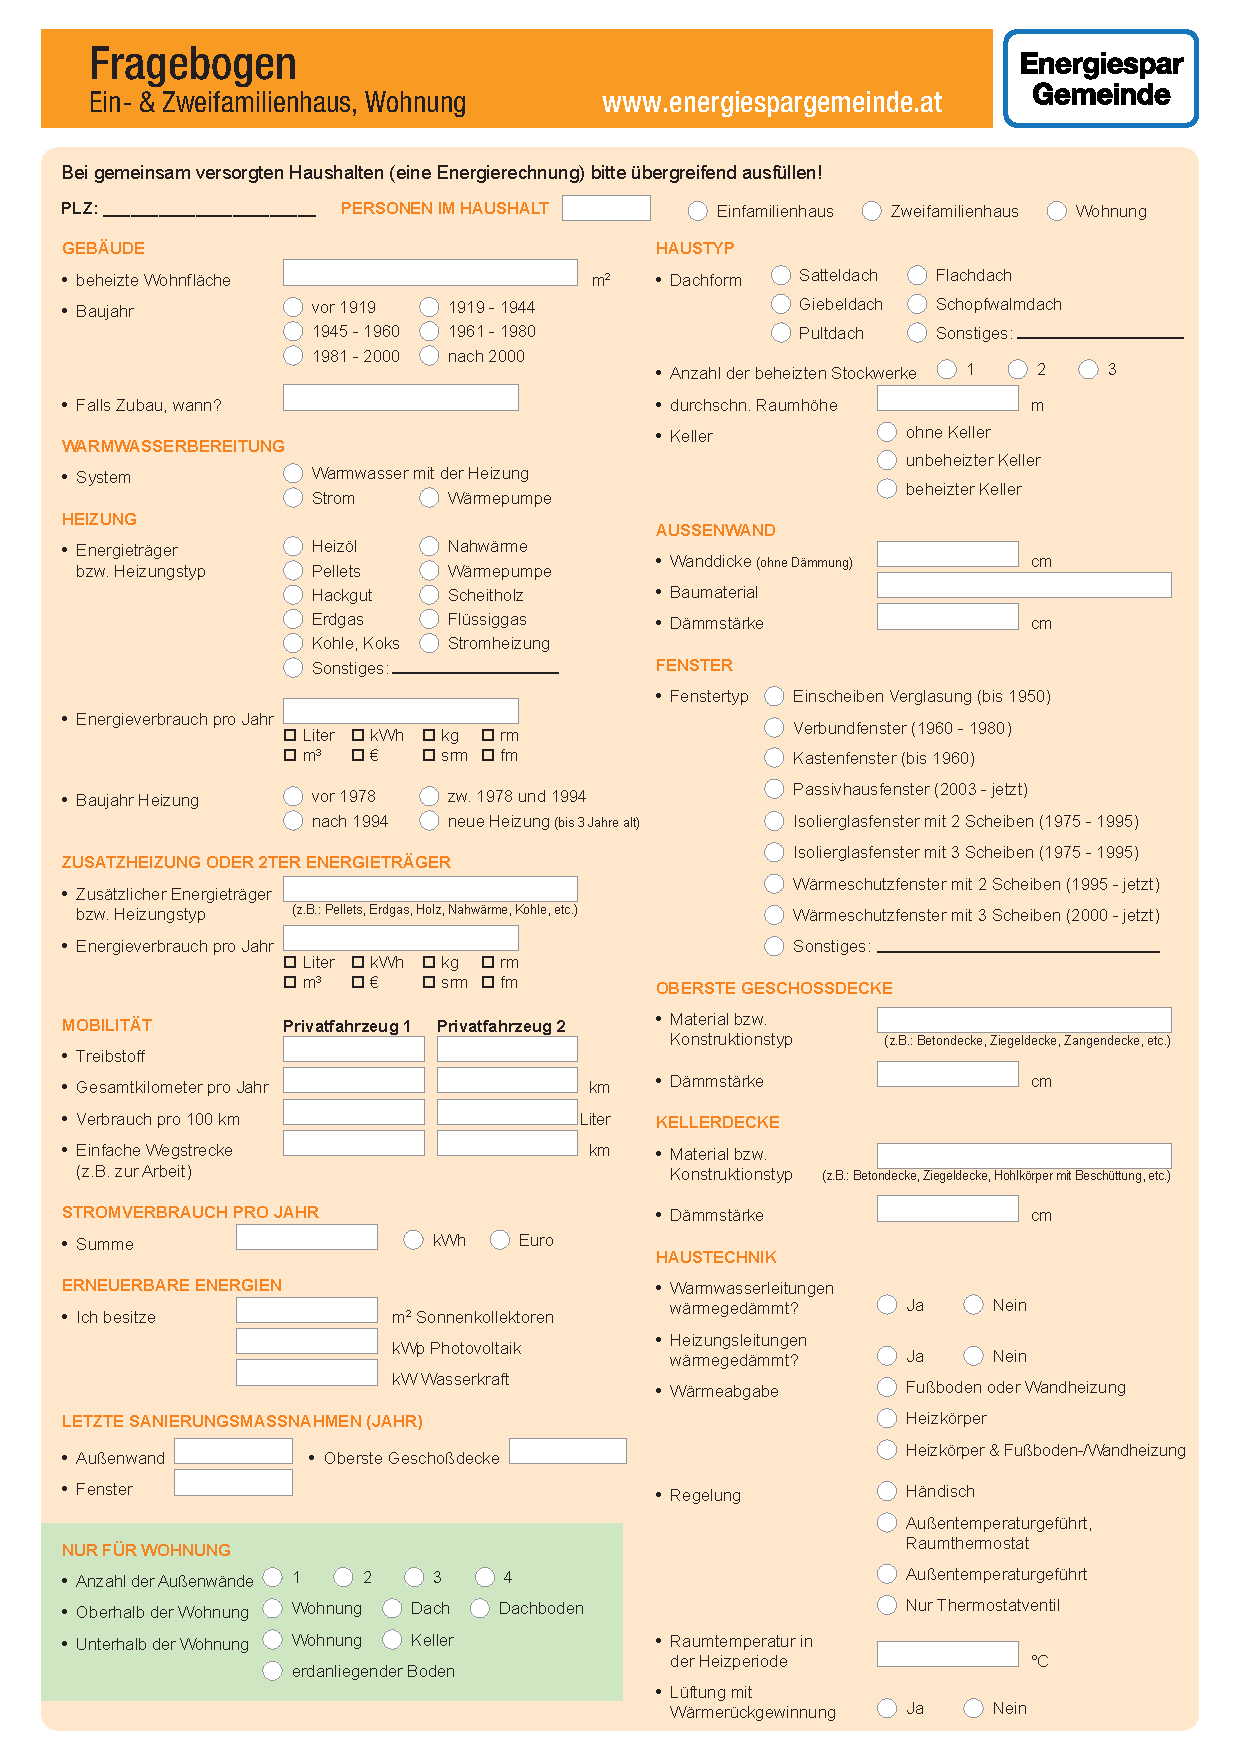
\includepdf[pages=1-,width=\textwidth,frame=true,pagecommand={}]{images/fragebogen}
\end{LaTeXCode}
%
The included pages are automatically scaled to the text width of the \latex document
by \verb!width=\textwidth! and \verb!frame=true! adds a surrounding border.

This example assumes that the external PDF document is in A4 page format.
With other formats you may have to adjust the scaling "manually" if the pages become
too tall (\eg, with \verb!width=0.9\textwidth!).

It is also important that all \emph{fonts} used in the external PDF document are
correct and fully \emph{embedded}, otherwise the PDF document generated by \latex may
not be viewable in another system environment!


\section{References to Included PDF Pages}

If you want to refer to specific pages in the included PDF, the easiest way is to import
single pages one by one and add a \emph{label} to each, as in this example:
%
\begin{LaTeXCode}[numbers=none]
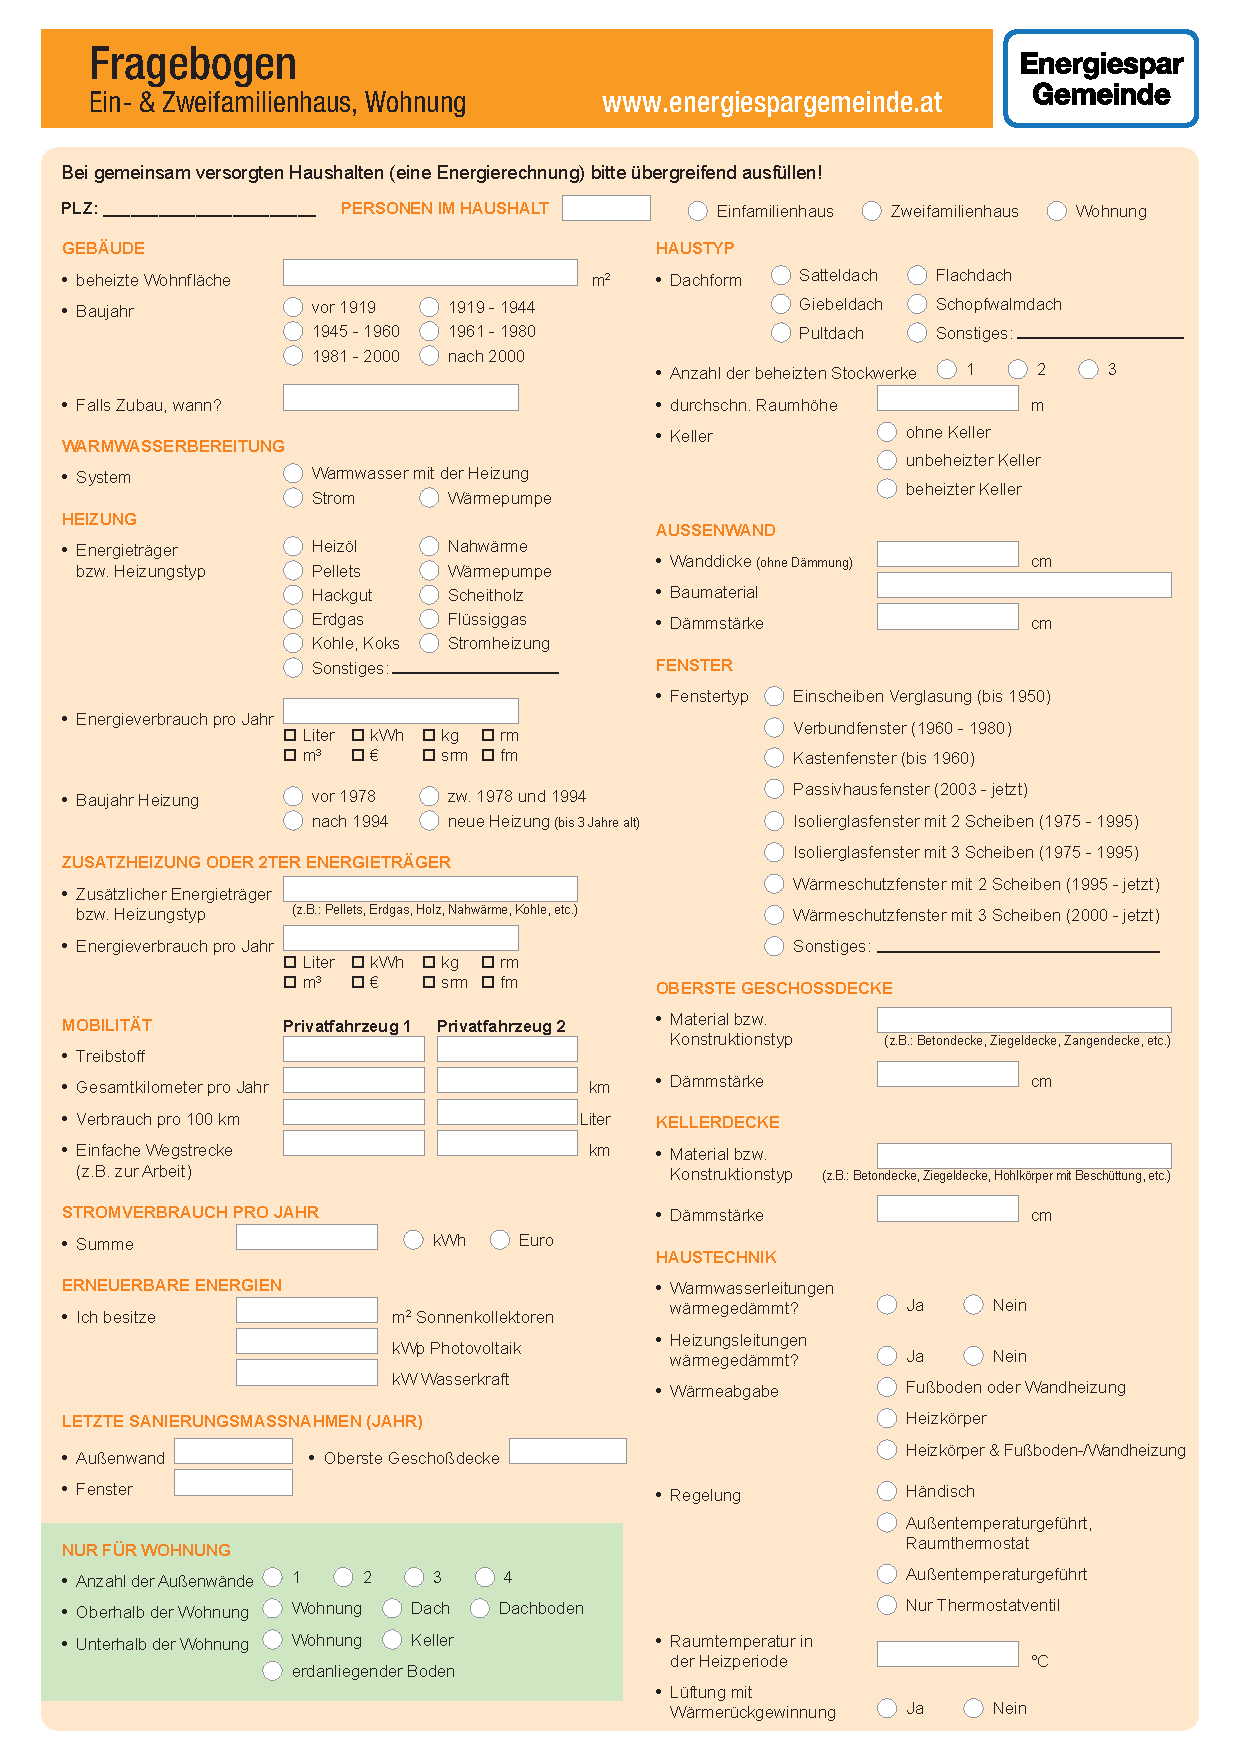
\includepdf[pages=1,width=\textwidth,frame=true,
		pagecommand={\label{PDF1}}]{images/fragebogen}
\includepdf[pages=2,width=\textwidth,frame=true,
		pagecommand={\label{PDF2}}]{images/fragebogen}
\end{LaTeXCode}
%
For example, in this case you could use \verb!\pageref{PDF2}! to specify the current page
number of the 2\textsuperscript{nd} page of the included PDF document. 
Many other options (\eg, specifying page intervals) can be found in the detailed documentation
for the \texttt{pdfpages} package.

% And here the foreign PDF document actually included:
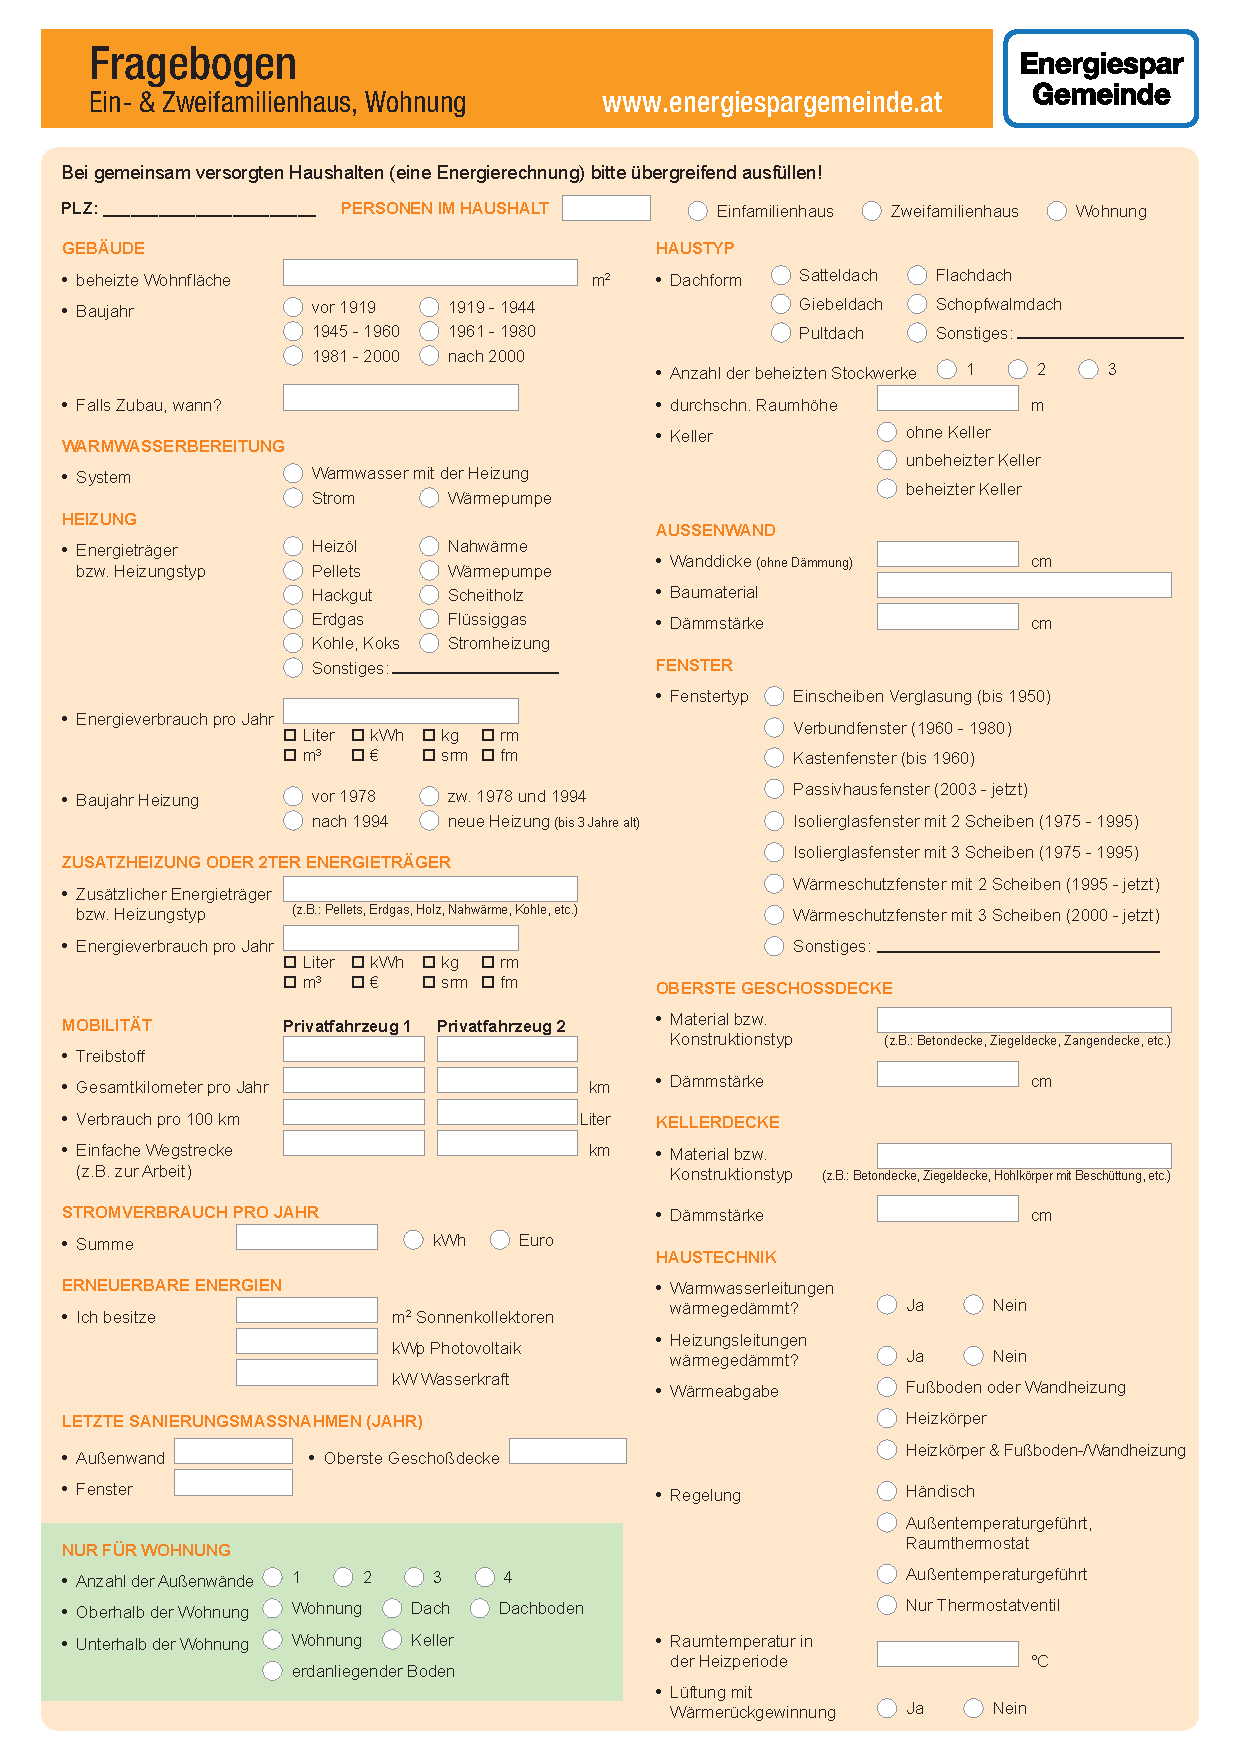
\includepdf[pages=1-,width=\textwidth,frame=true,pagecommand={}]{images/fragebogen}



 % Included other PDF document
%\chapter{\latex-Quellcode}
\label{app:latex}

\section*{Main File (\texttt{main.tex})}

\paragraph{Note:}
This should just be an \emph{example} of how to include source code in the
document's Appendix. It is accomplished with the following instructions:
%
\begin{LaTeXCode}[numbers=none]
\begin{footnotesize}
	\verbatiminput{main.tex}
\end{footnotesize}
\end{LaTeXCode}
%
Of course, the \latex source code of one's thesis is usually \emph{not} 
interesting enough to be reproduced here!

\begin{footnotesize}
	\verbatiminput{main.tex}
\end{footnotesize}





 % Source text of this document

%%%-----------------------------------------------------------------------------
\backmatter                           % Back part (bibliography, glossary, etc.)
%%%-----------------------------------------------------------------------------

\MakeBibliography % References

%%%-----------------------------------------------------------------------------
% Special page for checking print size
%%%-----------------------------------------------------------------------------

\chapter*{Measurement Box}



\begin{center}
{\Large --- Check the size of this box in your printout! ---}

\bigskip

\calibrationbox{100}{50} % Angabe der Breite/Hoehe in mm

\bigskip

{\Large --- Remove this page after printing and checking! ---}

\end{center}



%%%-----------------------------------------------------------------------------
\end{document}
%%%-----------------------------------------------------------------------------
